% --------------------------------------------------------------
% MarketMind — Final Project Report
% pdfLaTeX · Overleaf-ready · LAU MS Applied AI template
% --------------------------------------------------------------
\documentclass[12pt,a4paper]{report}

% --Encoding and fonts --
\usepackage[utf8]{inputenc}
\usepackage[T1]{fontenc}
% Default Computer Modern font (no font package needed)

% --Page geometry (LAU template: 1 in all sides) --
\usepackage[a4paper,margin=1in]{geometry}

% --Spacing --
\usepackage{setspace}
\onehalfspacing

% --Graphics and figures --
\usepackage{graphicx}
\graphicspath{{figures/}}
% SVGs pre-converted to PNG for Overleaf free-tier compatibility
\usepackage{float}
\usepackage[section]{placeins}  % auto \FloatBarrier at every \section boundary
\usepackage{subcaption}
\usepackage{needspace}          % \Needspace prevents stranded section headings

% --Tables --
\usepackage{booktabs}
\usepackage{array}
\usepackage{longtable}
\usepackage{tabularx}
\usepackage{multirow}

% --Bibliography --
\usepackage[numbers]{natbib}

% --TOC entry rendering (loaded before hyperref so \@starttoc redefinition order is correct) --
\usepackage[titles]{tocloft}   % used for "Appendix A" prefix in the TOC

% --Cross-references and links --
\usepackage[hidelinks]{hyperref}
\usepackage{cleveref}

% --Misc --
\usepackage{enumitem}
\usepackage{xcolor}
\usepackage{url}
\usepackage{textcomp}          % \textcopyright, etc.
\usepackage{parskip}           % paragraph spacing
\usepackage{etoolbox}          % patch chapter to remove forced page breaks
\usepackage{needspace}         % keep headings and nearby content together
\usepackage{seqsplit}          % allow long route names to break in narrow table cells
\usepackage{wrapfig}           % side-wrapped figures for tall portrait shots

% Stop \chapter from inserting a \clearpage so content flows continuously
\makeatletter
\patchcmd{\chapter}{\if@openright\cleardoublepage\else\clearpage\fi}{}{}{}
\makeatother

% Avoid orphaned section headings and keep floats from starting at a page bottom.
\pretocmd{\section}{\Needspace{8\baselineskip}}{}{}
\pretocmd{\subsection}{\Needspace{5\baselineskip}}{}{}
\pretocmd{\subsubsection}{\Needspace{6\baselineskip}}{}{}
\AtBeginEnvironment{figure}{\Needspace{12\baselineskip}}
\AtBeginEnvironment{table}{\Needspace{10\baselineskip}}
\AtBeginEnvironment{longtable}{\Needspace{10\baselineskip}}

% --Page-break hygiene: no widows, no orphans, no stranded last lines --
% Stops a single line (or the last sentence of a section) from being pushed
% alone onto the next page, and forbids a page break right after a hyphen.
\widowpenalty=10000
\clubpenalty=10000
\displaywidowpenalty=10000
\brokenpenalty=10000
% Let page bottoms run slightly short instead of stretching glue to fill them;
% this is what lets the high penalties above resolve into clean pages rather
% than "Underfull vbox" warnings.
\raggedbottom

% --Title data --
\newcommand{\reporttitle}{MarketMind}
\newcommand{\reportsubtitle}{Turning Real Customer Reviews into a Complete Advertising Campaign for Small Online Sellers}
\newcommand{\authorname}{William Radiyeh}
\newcommand{\supervisor}{Dr.\ Ahmad Hammoud}
\newcommand{\program}{Master of Science in Applied Artificial Intelligence}
\newcommand{\school}{School of Arts and Sciences}
\newcommand{\submissiondate}{May 2026}


% ==============================================================
\begin{document}

% --COVER PAGE --─────────────────────────────────────────────
\begin{titlepage}
\centering
\vspace*{1cm}

% LAU logo

\includegraphics[width=3in]{LAU-Logo-Green.jpg}\\[1.5cm]

{\LARGE \textbf{\reporttitle}}\\[0.4cm]
{\large \reportsubtitle}\\[2cm]

{\large By}\\[0.3cm]
{\Large \authorname}\\[2cm]

A project\\
submitted in partial fulfillment of the requirements\\
for the degree of \program\\[1cm]

\school\\[1cm]
\submissiondate

\vfill
\end{titlepage}


% --Front matter --───────────────────────────────────────────
\pagenumbering{roman}

% COPYRIGHT
\newpage
\begin{center}
{\large \textbf{Copyright}}
\end{center}
\vspace{0.5cm}
\textcopyright\ 2026, William Radiyeh. All rights reserved.

No part of this document may be reproduced, stored in a retrieval system, or transmitted in any form or by any means, electronic, mechanical, photocopying, recording, or otherwise, without the prior written permission of the author.

% PLAGIARISM STATEMENT
\newpage
\begin{center}
{\large \textbf{Plagiarism Policy Compliance Statement}}
\end{center}
\vspace{0.5cm}
I certify that:
\begin{enumerate}
\item I have read and understood LAU's Plagiarism Policy.
\item I understand that failure to comply with this Policy can lead to academic and disciplinary actions against me.
\item This work is substantially my own, and to the extent that any part of this work is not my own I have indicated that by acknowledging its sources.
\end{enumerate}

\vspace{1cm}
\noindent Name: \underline{\makebox[3in][l]{\,William Radiyeh}} \\[0.5cm]
\noindent Signature: \rule{3in}{0.4pt} \\[0.5cm]
\noindent Date: \underline{\makebox[3in][l]{\,14 May 2026}}

% ACKNOWLEDGEMENTS
\newpage
\begin{center}
{\large \textbf{Acknowledgements}}
\end{center}
\vspace{0.5cm}
I would like to thank Dr.\ Ahmad Hammoud for his careful supervision throughout this project, and for the time he spent reviewing each milestone in detail. His feedback shaped the way the system is described in this report and the way the experiments were framed.

I would also like to thank my family for their patience during the long writing and building stretches, and the LAU MS Applied AI faculty for the courses that prepared the ground for this work.

Any errors that remain in the report are my own.

% ABSTRACT
\newpage
\begin{center}
{\Large \textbf{\reporttitle}}\\[0.3cm]
{\large \authorname}\\[0.8cm]
{\large \textbf{Abstract}}
\end{center}
\vspace{0.5cm}

% Abstract on the 8-element structure: Background, Limitations of Literature, Problem
% Statement, Objective/Aim, Methodology, Key Results, Conclusion, Implications/Future Work.
% Three paragraphs, ~310 words, max one page. Round 6 rewrite (2026-05-14): P1 reopened
% with the platform definition per Hammoud's Round 6 feedback (main contribution = the
% platform, used consistently throughout the report); P2 keeps the offline / online
% description as a brief tour of the platform's components; P3 unchanged.
This thesis presents MarketMind, a review-intelligence platform that turns classified customer reviews into a complete Meta-style advertising campaign for small online sellers. Small sellers already have useful marketing evidence on every product page, yet they cannot read it at campaign speed. Generic AI copy tools produce fluent ad text but start from the seller's prompt rather than from buyer language, and they cover only the words on the ad. The alternative route, hiring a regional social-media agency, sits in the high hundreds of dollars per month on published GCC rate cards and is above what most one-person stores can absorb on a per-campaign basis. MarketMind fills the gap by grounding generation in real review evidence and producing the full campaign deliverable (copy, visuals, audience direction, funnel structure, and budget split) from a single short brief.

The platform has two halves connected by a single offline artifact. Offline, a DistilBERT classifier is fine-tuned on a product-aware split of 49,989 Amazon reviews across ten product categories; the trained model runs in batch to produce per-product sentiment profiles, curated review excerpts, and the inputs that a goal-aware product-ranking layer needs at runtime. Online, those inputs flow into a structured per-stage prompt that combines the user brief, brand assets, and curated review evidence, and the platform generates a three-stage Meta-style campaign through Gemini 3.1 Pro for copy and structured planning, Nano Banana Pro for portrait static images, and Veo 3.1 Fast for short video. The user-facing surface is a Next.js web application with an in-app evidence drawer that links every generated block back to the review excerpts that grounded it.

The fine-tuned DistilBERT classifier reached accuracy 0.872 and macro F1 0.673 against a TF-IDF and Logistic Regression baseline at 0.831 and 0.611, with the largest per-class gain on the underrepresented negative class. Qualitative ablations, one full campaign example and three further image-only examples across four product categories, judged against criteria taken from Meta's published creative best practices, showed that the structured review-grounded prompt produced more specific copy, cleaner visual composition, and tighter on-image text discipline than a generic prompt run against the same model. A per-campaign cost check on Google's published Gemini list prices put the API spend at roughly \$4.13 per complete campaign, two orders of magnitude below the cheapest published GCC agency retainer for a comparable creative volume. Future work covers a multi-rater evaluation across more product categories, paid Meta ad-spend testing, and brand-style fine-tuning for the visual generators.

\vspace{0.5cm}
\noindent\textbf{Keywords:} Review intelligence; sentiment analysis; DistilBERT; grounded language model generation; marketing automation.


% TABLE OF CONTENTS
\newpage
\tableofcontents

% LIST OF FIGURES
\newpage
\listoffigures

% LIST OF TABLES
\newpage
\listoftables


% ==============================================================
% MAIN MATTER
% ==============================================================
\newpage
\pagenumbering{arabic}

% --------------------------------------------------------------
\chapter{Introduction}
\label{ch:introduction}
% --------------------------------------------------------------

The main contribution of this thesis is MarketMind, a functional online web application that turns the customer voice already present on product pages into a complete Meta-style advertising campaign for small online sellers. It is delivered as a working platform rather than a study artifact: the seller opens the app and leaves with a finished campaign. The platform is built for the case where the seller has thousands of reviews on similar products and lacks the time or the team to turn that evidence into a launchable campaign. Inside the app the seller can generate a logo and a concept-product image, complete a six-step brief, read a review-intelligence screen that profiles their products, and receive a final campaign with Meta-style copy, generated visuals, an evidence drawer linking each block to its source reviews, and PDF, email, and dashboard delivery. The remainder of this chapter places the problem in context, names the parts of the gap that MarketMind closes, sets the project objectives, names the system-level contributions of the platform, and walks through the rest of the report.

\section{Domain and motivation}
\label{sec:domain}

The market that this project targets is small e-commerce: independent dropshippers, private-label brands, and one-person stores on Amazon, Shopify, Etsy, and similar platforms. Most of these sellers do not have a dedicated marketing team. They build ads in short bursts between fulfilment, customer support, and sourcing, and most of the writing happens from gut feeling.

At the same time, the customer voice that should be guiding these decisions already exists in plain sight on every product page. Reviews tell the seller which features people care about, which complaints come up the most, and which products earn loyalty. Sellers who read the reviews and write their ads from what buyers actually said tend to see the payoff in conversions, in repeat purchases, in lower refund rates, and in tighter creative briefs the next time around. Review data is therefore the right ground truth for full campaign decisions, because the same dataset answers four practical questions at once. Which product should be pushed first. Who is the buyer in their own words. What is the message that resonates. What objection should the ad address before the click. The same dataset informs product selection, audience targeting, copy, and visual direction.

Most ad-creation tools that a small seller can reach today focus on producing the words on the ad. Copy generators like Jasper and Copy.ai wrap general-purpose language models in a marketer-shaped interface. ChatGPT and Gemini do the same job for free if the seller knows what to ask. Image and video generators have caught up enough to matter too: Midjourney and Adobe Firefly produce print-ready static visuals, Nano Banana Pro renders legible on-image text, and short video models such as Veo and Sora produce usable eight-second clips from a written description. None of these tools, taken alone or together, draws on what real buyers wrote about the product. They make polished assets out of the seller's gut feeling, not out of evidence.

The economics of these tools matter more for a small seller than for a brand with a real marketing budget. Generated copy costs a fraction of a cent per call. Each generated image costs an order of magnitude more, and each short video clip costs another order of magnitude on top of that. A seller who runs ten copy variants sees no real bill; the same seller running ten image and video variants does. The pressure on a tool that serves the small-seller end of the market is therefore to pick the right creative on the first try, not to keep producing variants.

The other route a small seller could take, outsourcing the work to a social-media agency or a freelance designer, runs into the opposite economics. Published GCC rate cards put the cheapest fixed monthly package with design and captions at around \$340 per month (AED 1,249) for nine static posts and three short reels~\cite{si3packages}, with mid-tier industry guidance in the \$816--\$1,360 per month band (AED 3,000--5,000) for twelve to sixteen monthly posts~\cite{vpatchpricing}, and the floor rises to around \$2,176 per month (AED 8,000) once paid-ads management is bundled into the retainer~\cite{digitalwisepackages}. These retainers buy real services (account management, ongoing strategy, revision rounds, community management, performance reporting, and brand governance) that the platform described in this report does not pretend to provide. They are also priced for sellers whose monthly product sales clear the retainer comfortably, which is above what most one-person stores see in their first year. The practical effect is that creative iteration becomes a budget conversation each time the seller wants to try a new direction, and the default becomes whatever the previous campaign already looked like.

Large brands have already closed this loop internally. They have data teams who plug review and survey data into language models, copywriters who edit the output, and brand managers who push the result through paid agencies. They are not the audience for this project. The small seller who is also the founder, the customer-support agent, and the fulfilment manager is the audience. That seller already has the customer voice on the product page and a workable budget for ads. They do not have the time, the tooling, or the team to turn one into the other.

\section{Problem statement}
\label{sec:problem}

There are four parts to the problem, and they compound. The first part is that generic AI ad copy tools are not grounded in customer voice. They produce text that sounds polished but is often disconnected from what real buyers said about the product. A claim about a ``premium feel'' is meaningless if no review ever mentioned it.

The second part is that small sellers are missing more than the words on the ad. They are missing the full campaign stack. They need a logo if they do not have one yet. They need static images and a short video. They need an audience profile, a funnel structure that splits reach from sales, and a budget split across the funnel. They need a way to present the campaign cleanly to themselves or to a partner. A pure copy tool only solves a fraction of the problem.

The third part is cost, and it has two sides. The upstream side is the agency-and-freelance floor described in \cref{sec:domain}. A small seller who would happily pay an agency to produce ten polished posts a month is priced out before the conversation starts, which leaves doing it themselves with current generation tools as the only practical route. That route then runs into the downstream side. For a generic copy tool the per-call cost is so low that running ten variants is the rational default. The same default does not transfer to the visual side. A seller who generates ten static-image variants and three short video variants per campaign sees a bill that matters at the scale they are operating at. The pressure on the system is therefore to spend the visual budget once, in the right direction, rather than ten times across variants that do not differ enough to warrant the spend.

The fourth part is harder to see and rarely gets named. Generic copy tools do not show the seller why one variant is better than another, and they do not link the variant back to anything outside themselves. When the variant is wrong, the seller has no thread to pull. Adding a layer of review evidence behind the variant makes the link explicit. The headline can be read against the customer quote it came from, and the design direction can be checked against the complaint it is reframing. Without that link the system is another opaque generator. With it the system is a defensible piece of marketing reasoning.

This report describes a system that addresses all four parts. The technical core is a small trained sentiment classifier that turns reviews into a structured signal. The product wrapper takes that signal and feeds a complete campaign-production flow that covers branding, visuals, copy, targeting, funnel, budget, and delivery. The thesis the report defends is that grounding the generation step in this signal produces ad material that is more specific, more traceable, and more useful for a small seller than the same generation step run from a generic prompt, while a goal-aware product-ranking layer further keeps the visual generation budget tighter by picking the source evidence before any image is rendered.

\section{Objectives}
\label{sec:objectives}

The project pursues seven high-level goals, written as outcomes rather than as components of the system.

\begin{itemize}
  \item \textbf{O1.} Reduce the time and manual effort involved in planning a product-based digital ad campaign.
  \item \textbf{O2.} Examine how past customer reviews can be turned into something a marketer can actually use when planning a campaign.
  \item \textbf{O3.} Automate the path from a short user brief and review evidence to campaign material that is ready to launch.
  \item \textbf{O4.} Produce outputs that cover what real campaign execution requires: funnel strategy, audience direction, copy, and creatives.
  \item \textbf{O5.} Deliver each campaign at a per-call API spend low enough that a one-person store can iterate on creative without the cost asymmetry between text and visuals dominating the budget.
  \item \textbf{O6.} Test whether grounding generation in review evidence gives more specific and more useful output than a generic prompt.
  \item \textbf{O7.} Show the full approach as a working system that a non-technical user can take from brief to delivered campaign.
\end{itemize}

\section{Contributions of the thesis}
\label{sec:contributions}

The main contribution of this thesis is MarketMind: a review-intelligence platform that turns the customer voice on product pages into a complete Meta-style advertising campaign for small online sellers. The platform is the contribution at the level the project should be judged. The pieces inside it (the classifier, the curated review evidence, the goal-aware ranking layer, the structured prompt, the visual production wrapper, and the in-app evidence drawer) are component-level contributions that make the platform work; none of them, taken in isolation, is the contribution. \Cref{ch:approach} describes how the components are wired together.

The platform delivers eight system-level contributions, listed below. Each is written at the system level. The pieces inside each one are named only where naming them makes the contribution concrete.

\begin{itemize}
  \item \textbf{C1.} A review-intelligence platform that links customer review analysis to marketing campaign generation. The user provides a short brief and a target product, and the platform returns campaign material that is ready to use.
  \item \textbf{C2.} A trained sentiment classification model is the core intelligence layer of the platform. It is a fine-tuned DistilBERT classifier, benchmarked against a TF-IDF and Logistic Regression baseline, and trained on a product-aware split of 49,989 Amazon reviews drawn from ten product categories.
  \item \textbf{C3.} A review-evidence architecture that converts classified reviews into per-product sentiment profiles and curated review excerpts, then routes them through a goal-aware ranking layer with three strategies: highlight strengths, address objections, and differentiate. The campaign that comes out is tied to what customers actually wrote.
  \item \textbf{C4.} A campaign generation workflow that brings together brand identity, the curated review evidence, and the user brief inside a per-stage prompt with a fixed output schema. Each call returns audience direction, budget allocation, and copy for one stage of a Meta-style funnel.
  \item \textbf{C5.} A creative production workflow that extends generation beyond text. For every funnel stage the platform produces a 9:16 video and several 4:5 portrait static images, with two separate copy surfaces (text rendered onto the image, and a paste-ready caption for the ad platform). Brand assets feed the same workflow: an uploaded or in-app generated logo, a product image, a brand-guidelines PDF, and optional promo fields. A concept-product mode covers the case where the user does not yet have a real product photo.
  \item \textbf{C6.} An evidence-traceability layer inside the user interface. Every generated block is linked back to the review excerpts that grounded it through an in-app evidence drawer, so the campaign can be read line by line against its source material.
  \item \textbf{C7.} A qualitative comparison between a generic prompt and the structured review-grounded prompt, judged against criteria taken from Meta's published creative best practices: one full campaign-text and image example (YumSticks) plus three further image-only examples in other categories. The comparison reports specificity, traceability, and usefulness of the resulting ad material.
  \item \textbf{C8.} A working demo system that runs the whole pipeline for a non-technical user. It is a Next.js web application backed by the offline-trained model and the review-intelligence artifacts, with a personalised dashboard, auto-saving drafts, PDF export, and email delivery.
\end{itemize}

\section{Thesis structure}
\label{sec:structure}

\Cref{ch:related} places MarketMind inside the related research on sentiment analysis, transfer learning, evidence selection, structured prompting, and recent multimodal generation work, and closes by naming the specific gap that the platform is designed to address. \Cref{ch:approach} describes the platform itself. It opens with the platform-level solution overview, walks through the offline pipeline (the classifier, the per-product profiles, and the excerpt selection), then the runtime pipeline (the ranking layer, the structured prompt, the brand inputs, the targeting and budget, and the visual generation), and closes with the web application that delivers the platform to a non-technical user. \Cref{ch:results} reports results: the classifier comparison, the ranking sanity check, the generation comparison, the cost-effectiveness check, and a discussion of what worked and what did not. \Cref{ch:conclusion} closes with the limits of the current platform and a list of next steps.


% --------------------------------------------------------------
\chapter{Related Work}
\label{ch:related}
% --------------------------------------------------------------

MarketMind sits at the meeting point of four research strands and one applied area: sentiment analysis on noisy labels, transfer learning, evidence-based selection of text, structured prompting for grounded generation, and recent image and short-video generation models. This chapter walks through each strand, then closes with \cref{sec:gap}, which names the specific gap that the contributions in \cref{sec:contributions} are designed to address.

\section{Sentiment from review text}
\label{sec:sentiment}

Early work on sentiment analysis from product reviews used star ratings as a proxy label for opinion polarity, with bag-of-words features and shallow classifiers. Pang and Lee~\cite{pang2008opinion} surveyed the field through 2008 and laid out the standard pipeline: extract polarity-bearing terms, weight them, and fit a linear classifier. They also flagged the central failure mode of the approach. Lexical features alone cannot distinguish ``not bad at all'' from ``bad at all'' or read sarcasm. Their survey defined the baseline that every later method had to beat, and many of its observations about subjectivity, opinion mining, and aspect summarisation still hold.

Hu and Liu~\cite{hu2004mining} pushed the level of detail down from the review to the product feature. Their pipeline extracted frequent noun phrases as candidate features, attached opinion-lexicon hits to each feature, and produced per-feature sentiment summaries for products on shopping sites. The work introduced the practical question that aspect-based sentiment analysis still tries to answer. Do customers like the battery, the camera, or the screen, rather than the phone as a whole. Their lexicon-based pipeline broke down on noisy reviews, on negation, and on sarcasm, and most modern ABSA systems replace the lexicon with a fine-tuned classifier. MarketMind borrows the practical question (which features do buyers actually praise or complain about) but answers it with classified excerpts at the document level rather than aspect-tagged spans.

The release of large public review collections such as the Amazon Reviews 2023 dataset~\cite{ni2019justifying} made it possible to train modern models on a consistent corpus across many product categories. The full release covers more than 200 million reviews across 33 product categories. MarketMind takes a slice of 49,989 reviews across ten product categories, sampled from the most-reviewed products until each category reaches roughly 5,000 reviews. The labels in this corpus are still noisy. A 5-star review can carry a complaint about packaging, a 1-star review can include a backhanded compliment, and 3-star reviews mix praise and complaints in the same text. Any modern classifier trained on this kind of corpus has to deal with that noise rather than ignore it. The choice MarketMind makes is to keep the noisy labels as they are, lean on a stronger language model to absorb the noise during fine-tuning, and weight the loss function to compensate for the heavy class imbalance toward positive reviews (\cref{sec:dataset}, \cref{sec:distilbert}). The trade-off is a model that does not match a hand-cleaned single-domain benchmark but that generalises usably across ten categories at once.

\section{Transfer learning for text classification}
\label{sec:transfer}

Transfer learning made small training sets viable by separating the language model from the classifier. The Transformer architecture~\cite{vaswani2017attention} introduced self-attention as the backbone for sequence modelling and removed the recurrence that had made earlier sequence models slow to train and hard to parallelise. BERT~\cite{devlin2019bert} took the encoder half of the Transformer and pretrained it on a masked-language-modelling objective so the model learned bidirectional context, then fine-tuned a thin classification head on each downstream task. The result was strong scores on a wide range of GLUE benchmarks with only a fraction of the labelled data that an LSTM or CNN-text classifier would have needed. The recipe (general pretraining, task-specific fine-tuning) became the default for text classification within a year of release.

Two follow-up lines made the recipe practical at small budgets. DistilBERT~\cite{sanh2019distilbert} compressed BERT through knowledge distillation. A smaller student model is trained to match the soft-target outputs of the larger teacher, with an additional cosine-embedding loss that keeps the hidden representations aligned. The result is a model 40\,\% smaller that runs about 60\,\% faster while keeping roughly 97\,\% of BERT's downstream performance. ULMFiT~\cite{howard2018ulmfit} contributed two training-time tricks that DistilBERT users still rely on: discriminative fine-tuning (different learning rates for different layers) and slanted triangular learning-rate schedules. The tricks reduce catastrophic forgetting when adapting a pretrained model to a smaller labelled set, which matters at the scale that an MS project typically operates at.

MarketMind fine-tunes DistilBERT for two practical reasons. The model is small enough to train on a free Colab T4 GPU in under an hour, which keeps the project reproducible without paid hardware. The model is also large enough to handle the contextual cues that simple word counts miss: negation, sarcasm at the sentence level, and the difference between ``not bad'' and ``bad''. A baseline TF-IDF and logistic-regression model is trained on the same corpus as a sanity check (\cref{sec:baseline}). The DistilBERT model is the one whose outputs feed the rest of the pipeline because the gain over the baseline (accuracy 0.872 versus 0.831, macro F1 0.673 versus 0.611) is large enough to justify the modest extra training cost, and because a stronger sentiment signal makes every downstream step (theme extraction, ranking, prompt construction) more reliable.

\section{Picking representative review text}
\label{sec:picking}

Once a product has hundreds of reviews, the next problem is choosing which ones to feed downstream. Term weighting methods such as TF-IDF~\cite{sparckjones1972tfidf} have been the bedrock of unsupervised text selection since the early 1970s. Sp\"arck Jones argued that a term's importance in a document is inversely proportional to the number of documents it appears in across the corpus, and showed that the resulting weighting scheme outperformed plain term-frequency baselines on retrieval tasks. The formula is simple, has no learnable parameters, and runs at corpus scale on a laptop. Modern selection pipelines still use it as a cheap first pass before more expensive scoring.

A more recent line of work is aspect-based sentiment analysis (ABSA), which tries to attach sentiment to specific product features rather than to the whole review. The SemEval-2016 ABSA task~\cite{pontiki2016semeval} gave the field a shared evaluation across eight languages and seven domains, with three subtasks: sentence-level aspect detection, aspect-category sentiment, and out-of-domain generalisation. Zhang et al.~\cite{zhang2023absa} survey the field through 2023 and identify two structural shifts. The first is a move from pipeline systems (extract aspect, then classify sentiment) toward end-to-end multi-task models. The second is a move from feature-engineered classifiers toward fine-tuned language models. ABSA can produce output of the form (\textit{battery life, positive, ``lasts two days''}), which is closer to what an ad copywriter would want from a review than a single document-level polarity label.

MarketMind opted out of full ABSA for two reasons. The downstream task is sentence selection for a language model, not aspect labelling for a database, so the extra structure ABSA produces is wasted at the prompt-construction step where the language model is going to read the excerpt as text anyway. The second reason is data scarcity. The Amazon Reviews 2023 corpus does not come with aspect-level annotations, and labelling a usable training set in ten product categories is out of scope for an MS project. The pipeline therefore runs three lighter signals in sequence: classified sentiment polarity from the DistilBERT classifier (\cref{sec:distilbert}), TF-IDF weights computed per product on the cleaned review text, and a length window that filters out reviews too short to carry an opinion or too long to fit in the prompt budget. The output is a curated set of three to five excerpts per polarity per product, ready to be embedded in the campaign prompt.

\section{Structured prompting for grounded generation}
\label{sec:prompting}

Large language models are known to invent text that sounds confident but is not supported by any evidence. Brown et al.~\cite{brown2020gpt3} showed that scaling a Transformer language model to 175B parameters and conditioning it on a few well-chosen example pairs (few-shot prompting) lifts performance on a wide range of NLP tasks without any gradient updates. The paper reframed prompting as a first-class interface to language models: the prompt becomes the program, the example pairs become the demonstration, and the model becomes a contextual function. The same paper reported a strong sensitivity to prompt format, example ordering, and demonstration overlap, which is the empirical reason later work moved toward more explicit prompt structure rather than free-form natural-language instructions.

Retrieval-augmented generation (RAG)~\cite{lewis2020rag} adds a retrieval step so the model is conditioned on real source material. The architecture pairs a dense passage retriever with a sequence-to-sequence generator and is trained end-to-end so the retrieval is supervised by the downstream generation loss. RAG outperformed the closed-book BART baseline of similar size on open-domain question-answering tasks such as Natural Questions and TriviaQA, with substantially fewer fabricated answers. The pattern (retrieve-then-generate) became the default architecture for grounded question answering and for any application where the cost of an invented fact is high. RAG also exposed a limitation. When the retrieved passages disagree with each other, the generator has no built-in way to reconcile them, which is one reason production systems pre-process the retrieval set into a ranked, deduplicated, and structurally tagged form before passing it to the model.

Chain-of-thought prompting~\cite{wei2022cot} improves multi-step reasoning by exposing intermediate steps in the prompt. The original paper showed double-digit accuracy gains on arithmetic, commonsense, and symbolic reasoning benchmarks at the 540B-parameter scale, and the technique transferred to smaller models when the demonstrations were well chosen. The pattern that few-shot prompting, RAG, and chain-of-thought prompting share is that the prompt becomes a structured carrier of evidence and instruction rather than a single sentence. MarketMind follows the same pattern. The campaign-generation prompt (\cref{sec:structured}) is a fixed schema with named blocks for user identity, product context, campaign parameters, brand block, promo block, stage instructions, review-intelligence themes, supporting excerpts, and a JSON output schema. The blocks are composed at runtime from the per-product profile and the user's brief, and the model returns a strictly typed JSON object that the application parses without further freeform text.

\section{Image and video generation in marketing}
\label{sec:imagevideo}

Image generation moved from generative adversarial networks to diffusion models over the period 2020-2024. The dominant family is now denoising diffusion. A model is trained to reverse a noising process applied to natural images, conditioned on a text embedding from a paired text encoder. The output is high-resolution, prompt-faithful, and stylistically controllable. The capability that matters specifically for static advertising is on-image text rendering. Earlier diffusion models produced garbled letters at any resolution, which made them unusable for ad copy. Imagen 3 and Nano Banana Pro produce legible on-image text at sizes that survive a Meta feed crop. MarketMind uses Nano Banana Pro for the static portrait creatives. The choice is not load-bearing for the rest of the system: the structured prompt produces a typed copy block, and any image generator that can render text on the image can consume it.

Short-video generation reached a usable quality bar with the launch of Sora, Runway Gen-3, and Veo over 2024 and 2025. These models produce short clips with coherent motion, plausible lighting, and stable subjects across the duration of the clip. Current limits are well known. People speaking on camera still produce uncanny lip-sync. Motion across longer scenes drifts. Frame-to-frame consistency over thirty seconds is unreliable. Eight-second visual-only clips with a single subject and a single slow camera move are the sweet spot of the current generation. MarketMind treats the short video as the hero asset for the first creative block of each funnel stage, with the rest of the stage carried by static portrait images. The video model in production is Veo 3.1 Fast for cost reasons, and the same eight-second prompt template can be served by Sora or Gen-3 with no change to the upstream pipeline.

The marketing-specific gap that neither image nor video generators address is brand consistency. A general-purpose image model has no concept of the seller's brand, no memory of the seller's previous campaigns, and no obligation to produce visual variants that share a consistent palette, type, and mood. Solutions in production today either require the seller to upload a brand-style reference image, fine-tune a small adapter on a handful of brand assets, or pre-write detailed style instructions into every prompt. MarketMind goes the prompt route. The structured prompt accepts an optional product image, an optional brand-guidelines PDF, and an optional logo, and the upstream prompt builder turns those inputs into a design-direction block that the image model reads at generation time. The trade-off is honest: the brand consistency the system delivers is bounded by the prompt-following fidelity of the chosen image model, not by an explicit brand fine-tune.

\section{Research gap}
\label{sec:gap}

The reviewed work explains the pieces of the pipeline, but it does not show how those pieces become a seller-facing campaign system. Few existing systems tie a small trained sentiment classifier directly to a structured campaign-generation prompt and then wrap that combination inside a tool that also handles branding, visuals, targeting, budget, and delivery. Academic work tends to stop at one of the layers in isolation. Sentiment-classifier papers stop at the F1 score. RAG papers stop at the retrieval-grounded generation. ABSA papers stop at the aspect-tagged span. Commercial copywriting tools start at the prompt and skip the grounding step entirely. Jasper, Copy.ai, AdCreative, and the various ChatGPT marketing wrappers all expose a text-in / text-out box without any review pipeline behind it. The result is that a small seller who wants grounded, defensible ad material has to assemble five tools and most of the connective tissue by hand.

MarketMind tries to cover the full path from raw reviews to a deliverable campaign in one place, with the evidence trail visible to the user. The contribution is not the classifier, the prompt structure, the ranking layer, or the visual generator taken in isolation. The contribution is the end-to-end loop they form when they are wired together. A fine-tuned classifier produces the structured signal. A goal-aware ranking layer picks the source product. A structured prompt embeds the curated evidence. Current image and video models render the visuals. An in-app evidence drawer keeps every generated block linked back to the customer language that produced it. \Cref{ch:approach} describes how each link in that loop is built.

The gap is also economic, and not only technical. Published GCC agency rate cards put the cheapest credible monthly retainer for designed posts and captions at around \$340 per month (AED 1,249) for nine static posts and three short reels~\cite{si3packages}, rising to around \$2,176 per month (AED 8,000) once paid-ads management is included~\cite{digitalwisepackages}. The academic systems and commercial copy tools named earlier in this chapter do not move that floor. They either skip designed visuals entirely, or they sit at consumer-subscription price points that still assume a user who can afford to retry generation many times over. A system that produces a complete review-grounded campaign at the per-call cost of a few static images and a few seconds of generated video on a public model API is therefore a different kind of intervention. \Cref{sec:cost} returns to that comparison after the model and generation results are in, and frames it as an order-of-magnitude viability check rather than a like-for-like substitute claim.


% --------------------------------------------------------------
\chapter{The MarketMind Platform}
\label{ch:approach}
% --------------------------------------------------------------

Each of the eight contributions named in \cref{sec:contributions} corresponds to one or more components of the MarketMind platform described in this chapter. The chapter walks the platform along its natural lifecycle. \Cref{sec:solution} opens with a platform-level solution overview, framed as an extended prose version of \cref{sec:contributions}. \Cref{sec:arch} gives the architecture diagram. \Cref{sec:offline} describes the offline pipeline that produces the review-intelligence artifact: the dataset and preprocessing, the baseline and main classifiers, and the curated excerpt selection. \Cref{sec:runtime} describes the runtime pipeline that turns the artifact and the user brief into a campaign: the goal-aware ranking layer, the structured prompt, the brand inputs, the targeting and budget, and the visual generation. \Cref{sec:web} covers the web application that delivers the platform to a non-technical user, from the user journey through the implementation and runtime.

\section{Solution overview}
\label{sec:solution}

MarketMind is a single review-intelligence platform with one job: turn the customer voice on product pages into a complete Meta-style advertising campaign that a small online seller can launch from a short brief. Everything inside the platform serves that one job. MarketMind is delivered as a functional online web application, not a pipeline script or a report artifact: a non-technical seller uses it through a browser, from the first screen to the exported campaign. This section gives an extended prose version of the contributions listed in \cref{sec:contributions}, framed at the platform level before the architecture diagram appears in \cref{sec:arch}.

The platform is built around three commitments that distinguish it from a generic prompt-driven tool. The first commitment is that customer reviews are the primary source of truth for every creative choice. Sellers do not lack ad-copy generators; they lack ad copy that comes from what real buyers said about the product. MarketMind is therefore not a prompt-only tool. It is a small data pipeline with a generation step at the end. The trained sentiment classifier and the per-product profiles are not auxiliary to the platform; they are the centre of what the platform does.

The second commitment is that the platform splits its work in time. The classifier and the per-product profiles are computed once, offline, and stored as a single artifact (\cref{sec:offline}). The runtime reads from that artifact (\cref{sec:runtime}). This split keeps the user-facing latency low even though the underlying review corpus is large, and it keeps the online half simple enough to walk through in a single diagram.

The third commitment is that the platform delivers the full campaign deliverable, not just the copy. A small seller does not need three more headline variants. They need a logo if they do not have one, a product image, a short video, several portrait static images with on-image text, an audience profile, a funnel structure, a budget split across the funnel, and a way to deliver the result to whoever is going to launch it. The platform is built so that the same review evidence that grounds the copy also drives the design direction, the audience direction, and the budget allocation.

The user-facing flow is short. The seller submits a brief, attaches whatever brand assets they have, picks a source product from a ranked review-intelligence shortlist, and reviews the generated three-stage Meta-style campaign. Every block in that view is linked back to the review excerpts that grounded it through an in-app evidence drawer (\cref{sec:web}); the seller can save the campaign as a draft, export the report as a PDF, or send it by email.

\section{Architecture overview}
\label{sec:arch}

MarketMind has two halves separated by what is computed when. The offline half runs once during preprocessing and produces a single artifact that the online half consumes. The online half runs every time a user starts a campaign. \Cref{fig:architecture} shows the architecture; the four paragraphs after the figure walk through it.

\begin{figure}[ht!]
  \centering
  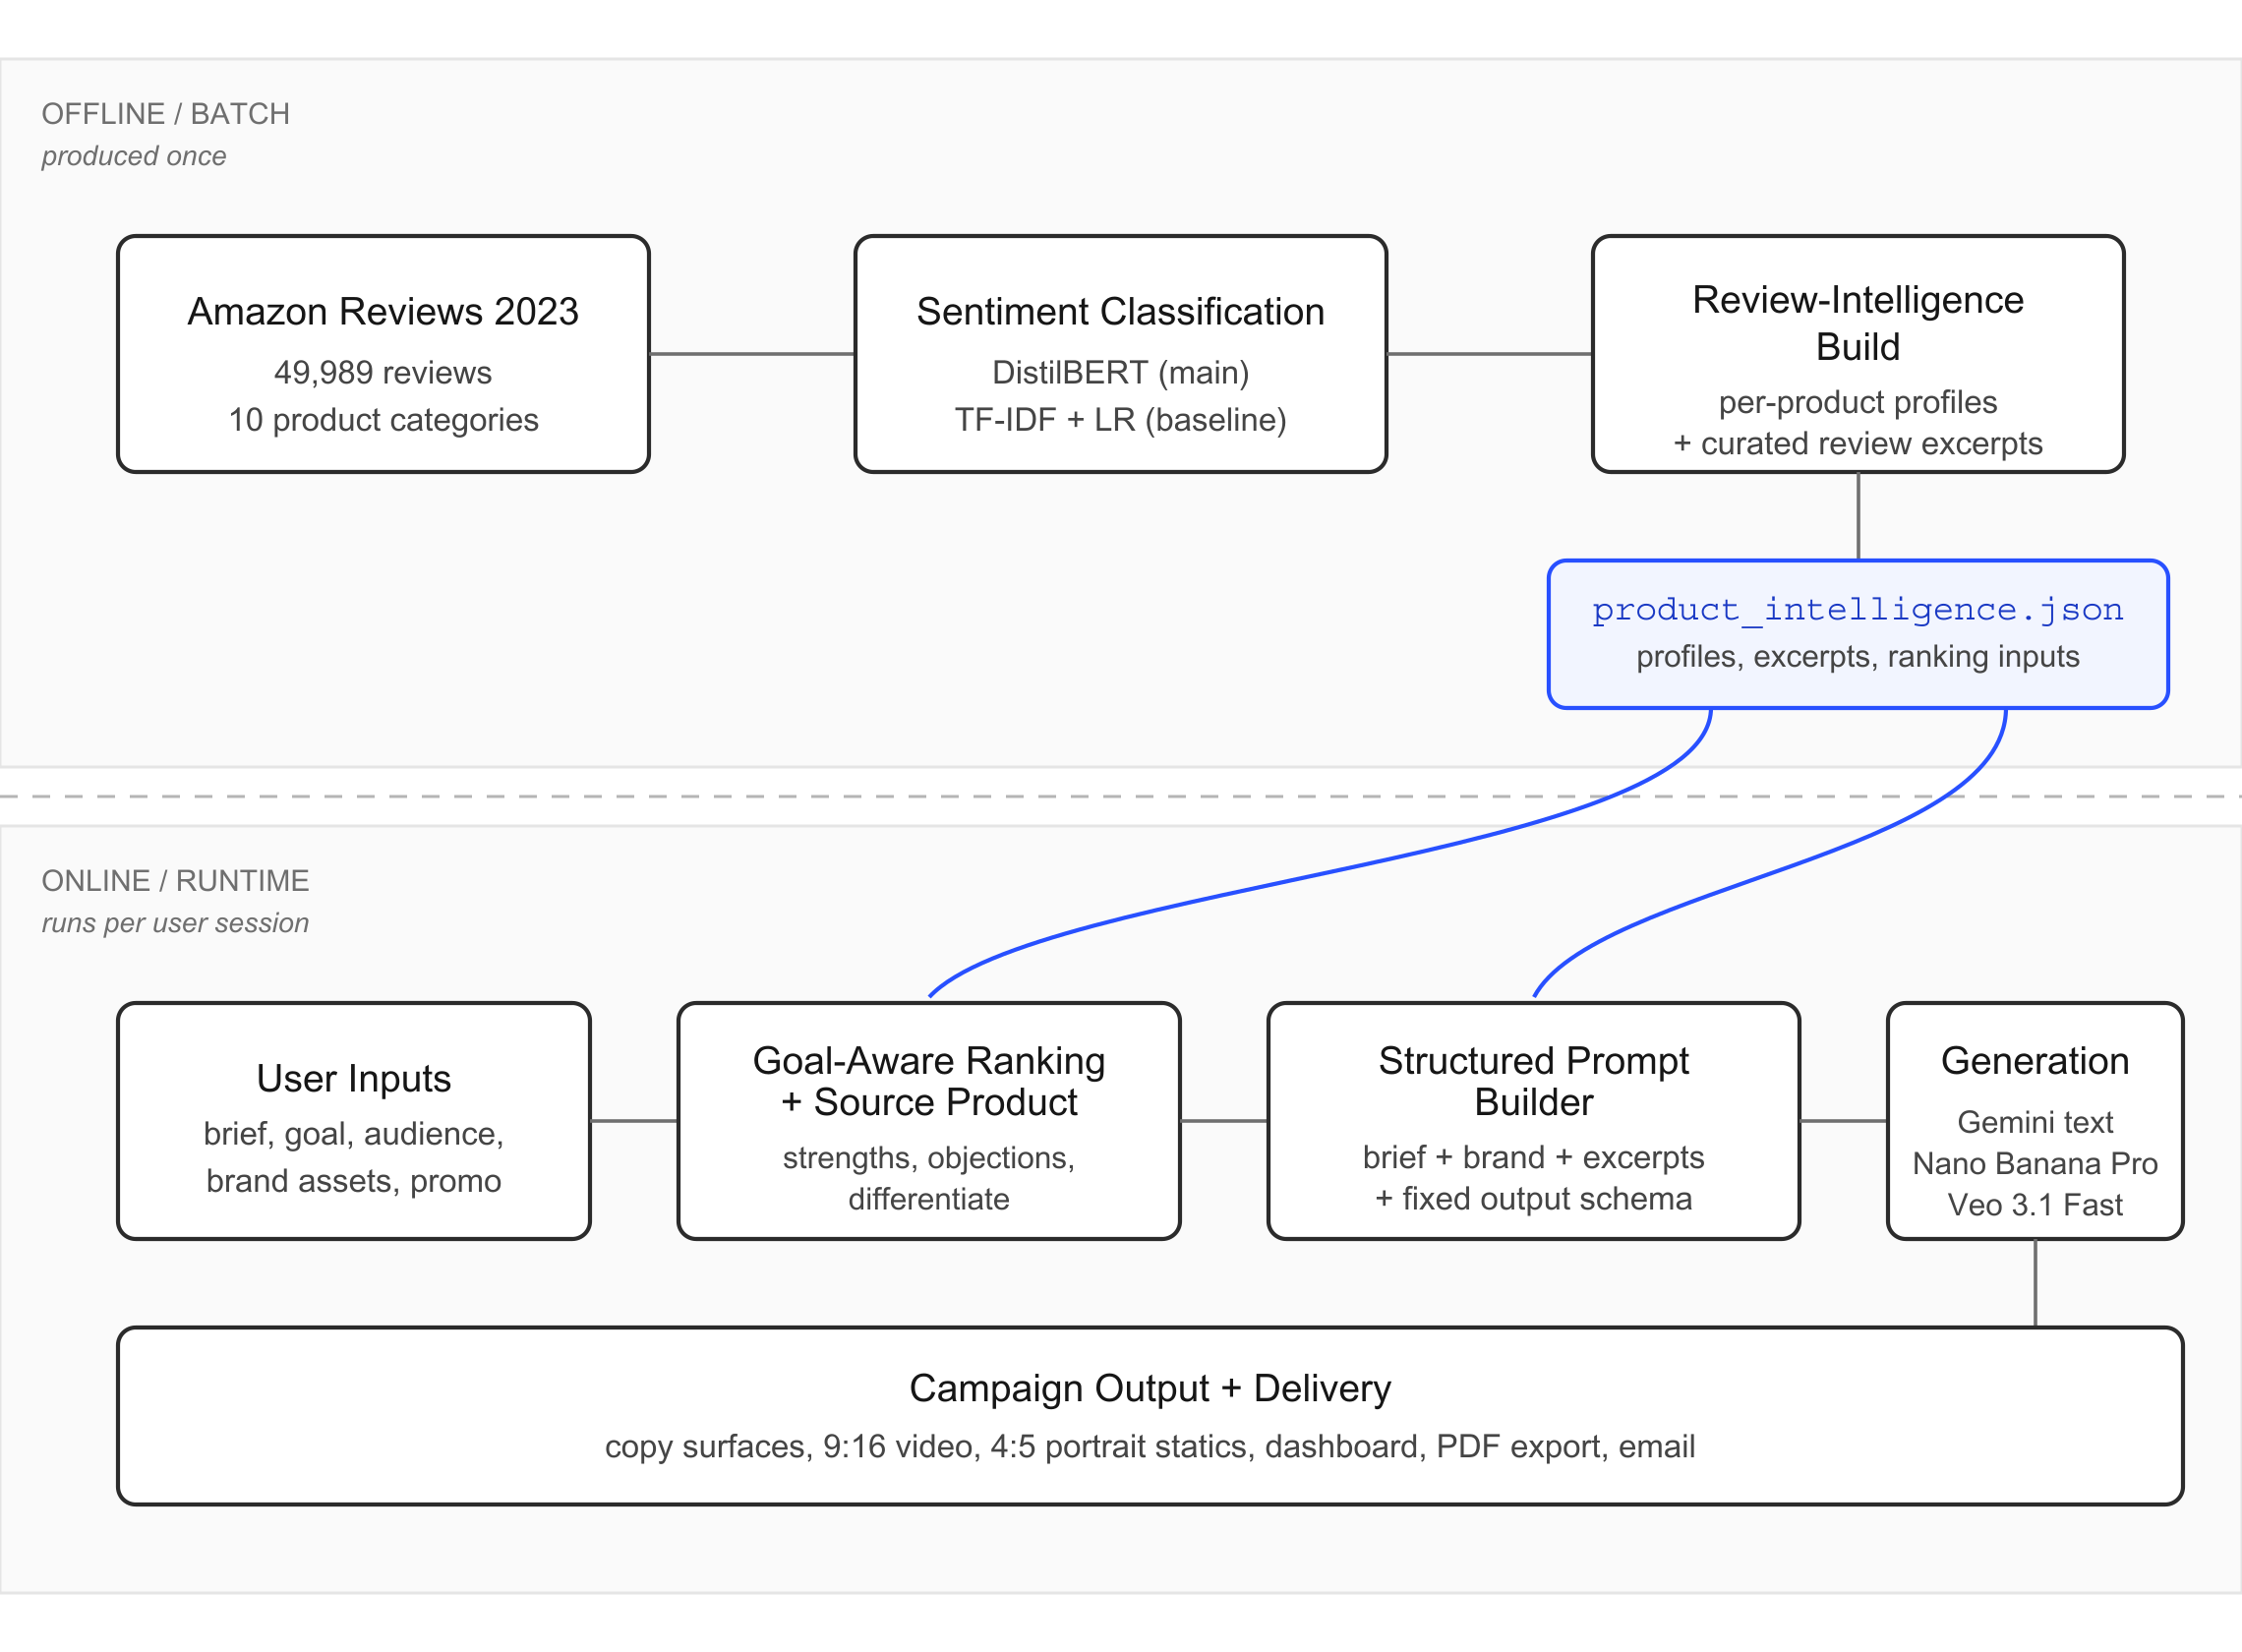
\includegraphics[width=\textwidth]{architecture-overview}
  \caption{MarketMind system architecture. The offline build (top lane) runs once and produces \texttt{product\_intelligence.json}. The online runtime (bottom lane) consumes it per user session. Dark arrows mark the flow that crosses the boundary.}
  \label{fig:architecture}
\end{figure}

The offline half ingests the review corpus, trains the sentiment classifier (DistilBERT as the main model, TF-IDF and Logistic Regression as the baseline), and runs the trained model in batch over the full dataset. The output is a single artifact, \texttt{product\_intelligence.json}, that holds per-product sentiment profiles, curated representative excerpts, and the inputs that the goal-aware ranking layer needs at runtime. After this point, the raw 49,989 reviews are not touched again.

The online half starts with the user's brief and brand assets. The goal-aware ranking layer reads the artifact, scores similar products against the chosen campaign goal under one of three strategies (highlight strengths, address objections, or differentiate), and lets the user pick a source product.

The structured prompt builder then assembles a per-stage prompt that combines the user brief, the brand inputs, the curated excerpts for the chosen product, and a fixed output schema. One call is made per funnel stage, so each call stays focused on a single stage of a Meta-style funnel and returns audience direction, budget allocation, and the copy for that stage.

Generation is a single multimodal step per stage. Gemini produces text, Nano Banana Pro produces 4:5 portrait static images, and Veo 3.1 Fast produces a short 9:16 video. Outputs land in the campaign view, where they can be reviewed inside an evidence drawer that links every block back to its source excerpts, exported as a PDF, emailed, or saved to a personalised dashboard. Each block in the architecture is a separate module so the system can be inspected, tested, and replaced one piece at a time. \Cref{sec:dataset} onward describes each module in turn.

\section{Offline pipeline: review intelligence}
\label{sec:offline}

The offline pipeline is the half of the platform that runs once, before any user touches the application. It turns a raw corpus of Amazon reviews into the single review-intelligence artifact (\texttt{product\_intelligence.json}) that the runtime reads on every campaign. Four steps make up the pipeline: a sampled and cleaned dataset (\cref{sec:dataset}), a baseline TF-IDF and Logistic Regression classifier (\cref{sec:baseline}) for comparison, a fine-tuned DistilBERT classifier (\cref{sec:distilbert}) as the main model, and a curated excerpt selection step (\cref{sec:excerpts}) that picks the reviews each downstream prompt will see. The output of the four steps is the per-product sentiment profile and the curated set of positive, neutral, and negative excerpts that the runtime carries into the structured campaign prompt.

\subsection{Dataset and preprocessing}
\label{sec:dataset}

The data comes from the Amazon Reviews 2023 release. Ten product categories were chosen to give the classifier a wide enough domain mix without bloating the training run: Baby Products, Beauty and Personal Care, Electronics, Health and Household, Home and Kitchen, Office Products, Pet Supplies, Sports and Outdoors, Tools and Home Improvement, and Toys and Games. From each category, the most-reviewed products were sampled until the slice reached approximately 5,000 reviews, then merged. Empty reviews were dropped, leaving 49,989 cleaned reviews in total.

Star ratings were collapsed into three sentiment classes following the standard convention used in earlier review-sentiment work: 4--5 stars become positive, 3 stars become neutral, and 1--2 stars become negative. The resulting class distribution is heavy on the positive side, which matches the natural skew of the dataset: positive 84.5 percent, negative 9.1 percent, and neutral 6.4 percent.

\begin{figure}[ht!]
  \centering
  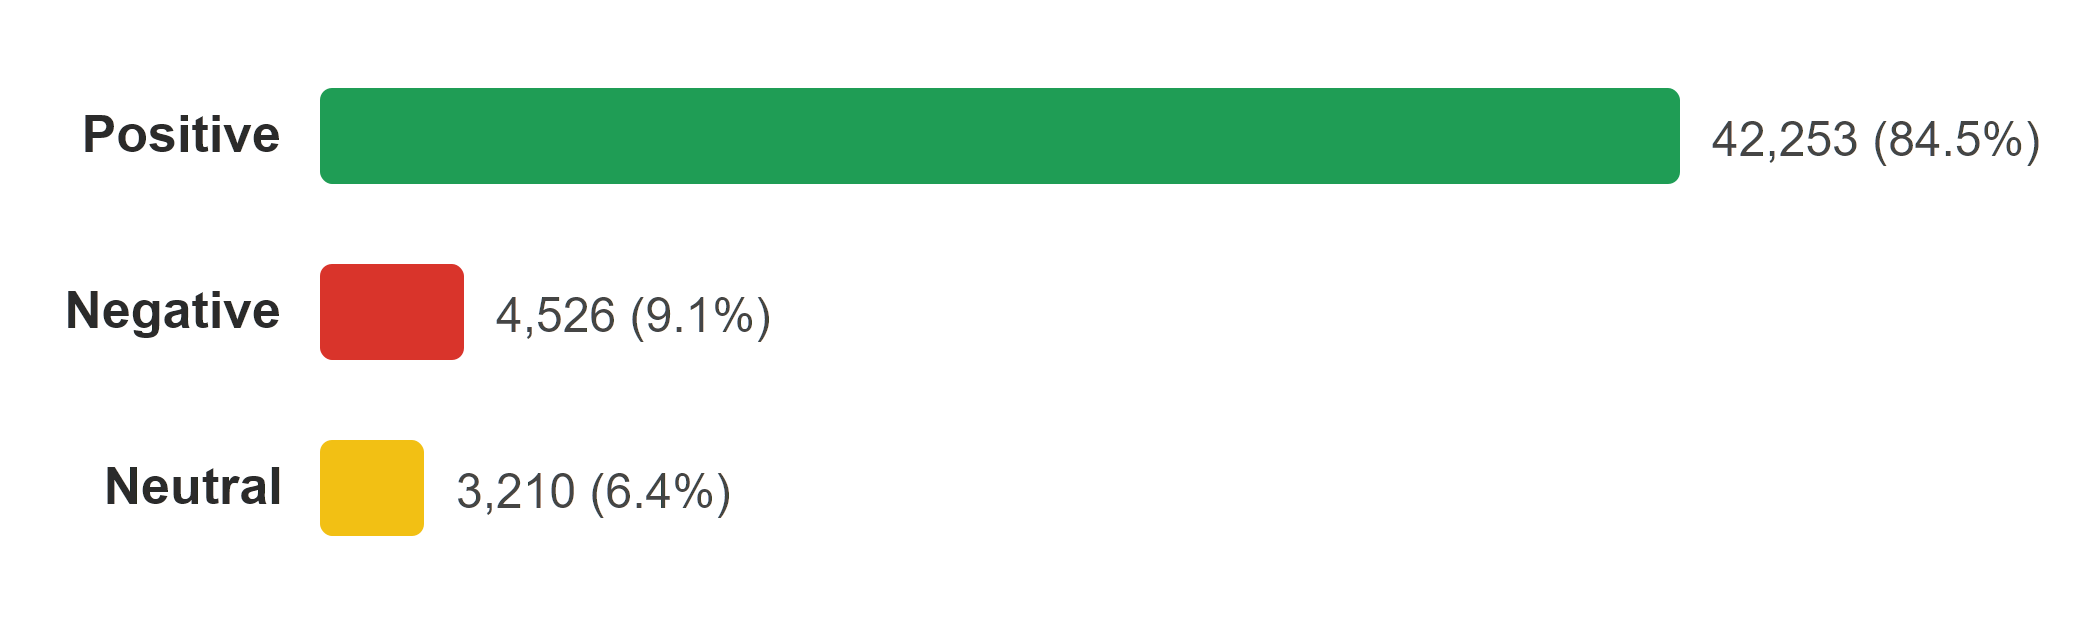
\includegraphics[width=\textwidth]{class-distribution}
  \caption{Class distribution across the cleaned 49,989-review dataset. Imbalance ratio is roughly 13 to 1 between positive and neutral.}
  \label{fig:classdist}
\end{figure}

Two preprocessing decisions are worth highlighting because they shape the rest of the chapter. The first is class weighting. Without it, any model trained on this data would default to predicting ``positive'' for every input, since that alone gives an 84 percent accuracy. Weighted cross-entropy loss makes the rarer classes count more during training. The second decision is a product-aware train/validation/test split. A naive random split would leak product-specific wording across the three sets, since many products have multiple reviews. The data was split at the product level (using GroupShuffleSplit on the product identifier) so no product appears in more than one set. The model therefore has to generalise from review language, not from memorised product wording.

\begin{table}[ht!]
  \centering
  \caption{Dataset summary.}
  \label{tab:dataset}
  \begin{tabular}{@{}ll@{}}
    \toprule
    Field & Value \\
    \midrule
    Source & Amazon Reviews 2023 (public release) \\
    Categories & 10 \\
    Reviews after cleaning & 49,989 \\
    Unique products & 4,173 \\
    Products with at least 10 reviews & 1,357 \\
    Reviews covered by those 1,357 products & 32,247 (64.5\%) \\
    Mean reviews per product & 12.0 (median 7.0) \\
    Largest single product & 1,518 reviews \\
    \bottomrule
  \end{tabular}
\end{table}

\subsection{Baseline classifier (TF-IDF + Logistic Regression)}
\label{sec:baseline}

The baseline is intentionally simple. The text is vectorised with TF-IDF (50,000 maximum features, unigrams and bigrams, sublinear term-frequency scaling) using scikit-learn~\cite{sklearn2011}. A Logistic Regression classifier is then trained on top with \texttt{class\_weight} set to ``balanced'' to absorb the imbalance. Training takes about 13 seconds on the local machine. The role of the baseline is not to win; it is to set a clear floor that any heavier model has to beat in order to justify its training cost.

\subsection{Main classifier (fine-tuned DistilBERT)}
\label{sec:distilbert}

The main classifier is a fine-tuned DistilBERT model (\texttt{distilbert-base-uncased}, 66 million parameters). The text is tokenised at a maximum length of 256 tokens, which covers most reviews without truncation. Training uses weighted cross-entropy loss with class weights set inversely proportional to class frequency: roughly 0.39 for positive, 3.72 for negative, and 5.27 for neutral. The optimiser is Adam with a learning rate of 2e-5, a 10 percent linear warmup, batch size 32, and three epochs. Training runs on a free Colab T4 GPU and takes about 38 minutes.

The validation set is used only for epoch selection. The test set is seen exactly once, at the end. The best epoch on validation macro F1 is epoch 2.

\begin{figure}[ht!]
  \centering
  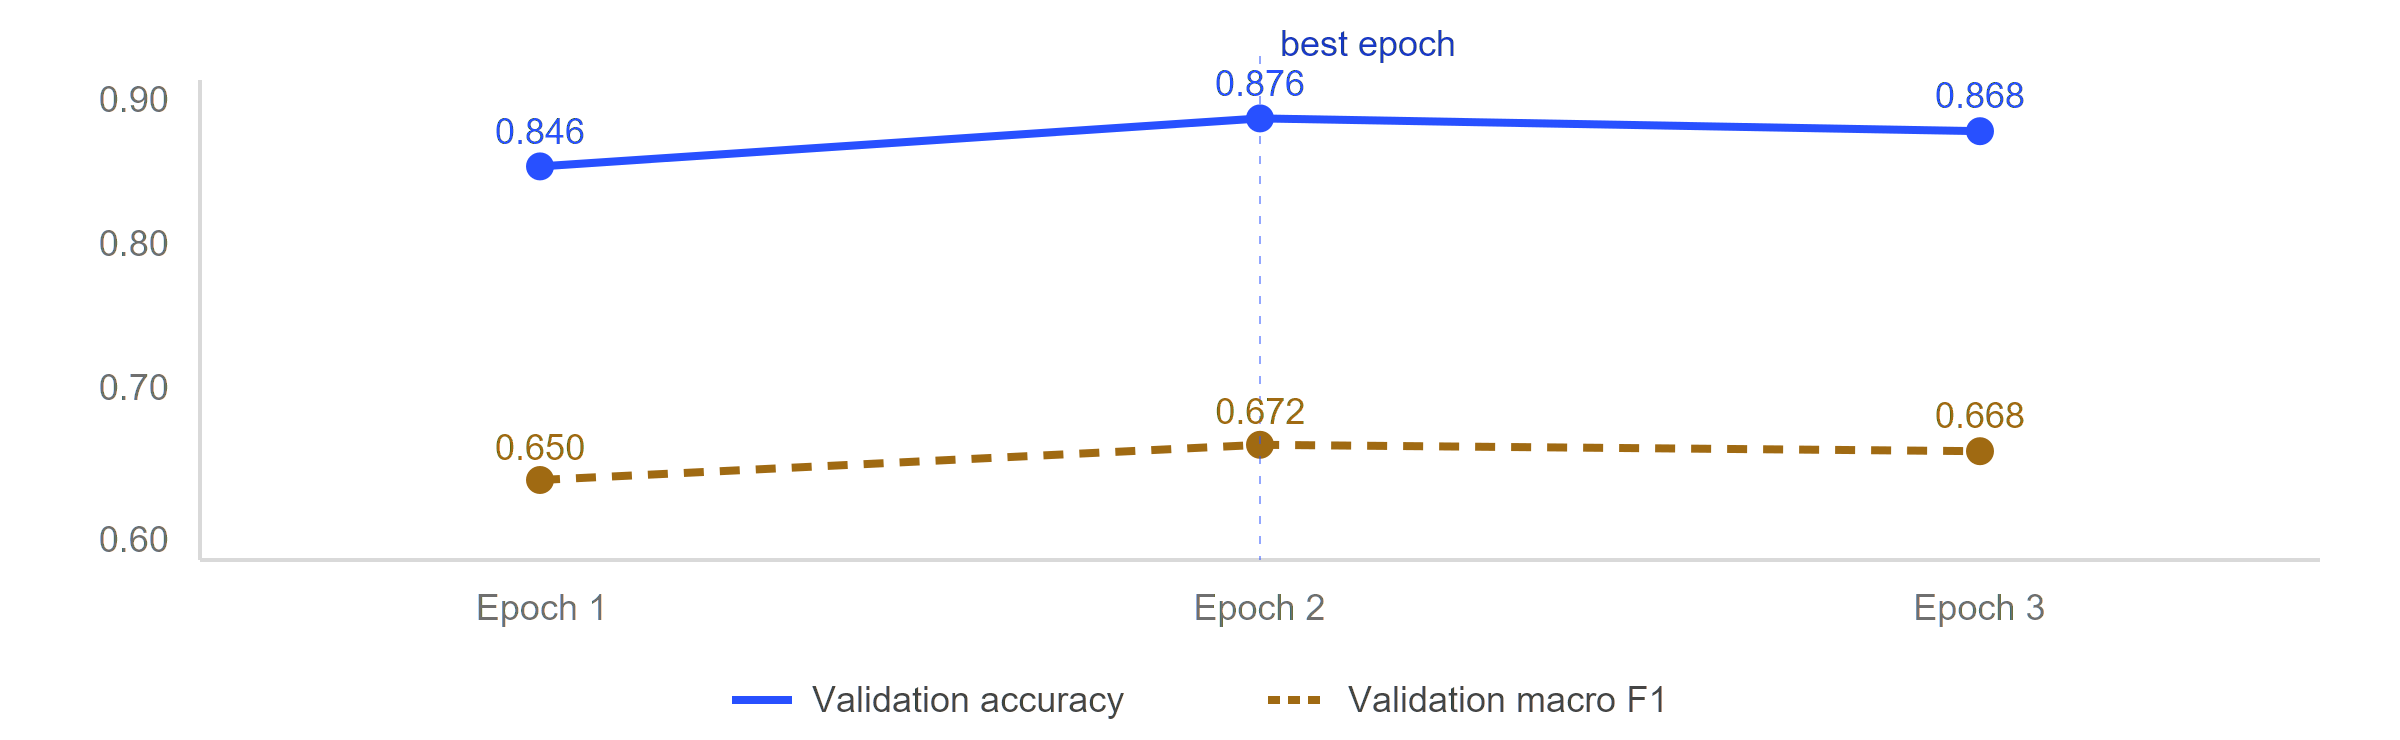
\includegraphics[width=\textwidth]{validation-curves}
  \caption{Both metrics peak at epoch 2 and dip slightly at epoch 3, which is why epoch 2 is selected.}
  \label{fig:valcurves}
\end{figure}

\subsection{Picking the right reviews to show the language model}
\label{sec:excerpts}

Once every review has a predicted label, each product is reduced to a sentiment profile: the percentage of reviews in each class plus the total review count. For the 1,357 products with at least ten reviews, this gives a stable summary that downstream steps can work with. Across these 1,357 products, the predicted distribution is approximately 80 percent positive, 10 percent neutral, and 10 percent negative.

The next step is selection. A language model cannot read every review, and a pure summary loses the customer voice. The system therefore picks a small set of representative excerpts per sentiment group, using a simple TF-IDF score over the product's reviews. The selection rules are short and transparent: order the candidate reviews in each sentiment group by classifier confidence, drop reviews that are too short to be informative, drop near-duplicates (reviews whose first 120 normalised characters match an earlier pick), and keep filling each group up to a target count. The output is a small evidence pool per product that the language model sees as part of its prompt.

The number that matters for the user interface is the size of that pool. The campaign-output screen rotates excerpts across eleven creative blocks, so the pools are sized to give every block at least one fresh excerpt where possible: up to 22 positive excerpts, up to 22 negative, and up to 11 neutral per product. These targets are bounded by what the data actually contains; for a product with only a handful of negative reviews, the negative pool will be smaller. The interface flags this case to the user rather than inventing variety.

\section{Runtime pipeline: campaign generation}
\label{sec:runtime}

The runtime pipeline is the half of the platform that fires every time a user starts a campaign. It reads the review-intelligence artifact produced offline (\cref{sec:offline}), combines it with the user's brief and brand inputs, and returns a three-stage Meta-style campaign with copy and visuals on each stage. The pipeline runs in a short sequence: a goal-aware product ranking layer picks the source product (\cref{sec:ranking}), a structured prompt carries the curated evidence into the language model (\cref{sec:structured}), and the brand inputs, the targeting and budget split, and the visual generation follow as the closing runtime steps (\cref{sec:brand}).

\subsection{Goal-aware product ranking}
\label{sec:ranking}

The user picks a campaign goal at the start. Three goals are supported: highlight strengths, address objections, and differentiate. The same set of similar products is then reordered under three simple ranking formulas:

\begin{itemize}
  \item \textbf{Highlight strengths.} 60 percent positive percentage plus 40 percent volume score. Surfaces products that are well loved by enough buyers to make the praise representative.
  \item \textbf{Address objections.} 50 percent mixed-sentiment score plus 50 percent volume score. Surfaces products with a real share of complaints, which is what an objection-handling campaign needs to engage with.
  \item \textbf{Differentiate.} 70 percent distinctiveness plus 30 percent volume score. Surfaces products whose review language stands apart from the rest of the category.
\end{itemize}

The ranking layer is algorithmic and transparent, not learned. The sanity check in \cref{ch:results} measures Top-N Jaccard overlap across the three rankings to confirm that the goal really does change which products surface.

\subsection{Structured prompt for grounded campaign generation}
\label{sec:structured}

The contribution on the language-model side is the prompt itself. Instead of one generic instruction (``write an ad for this product''), the system builds a structured prompt with named blocks. Each block has a fixed role. The model fills in the output schema rather than free-form text.

\begin{figure}[ht!]
  \centering
  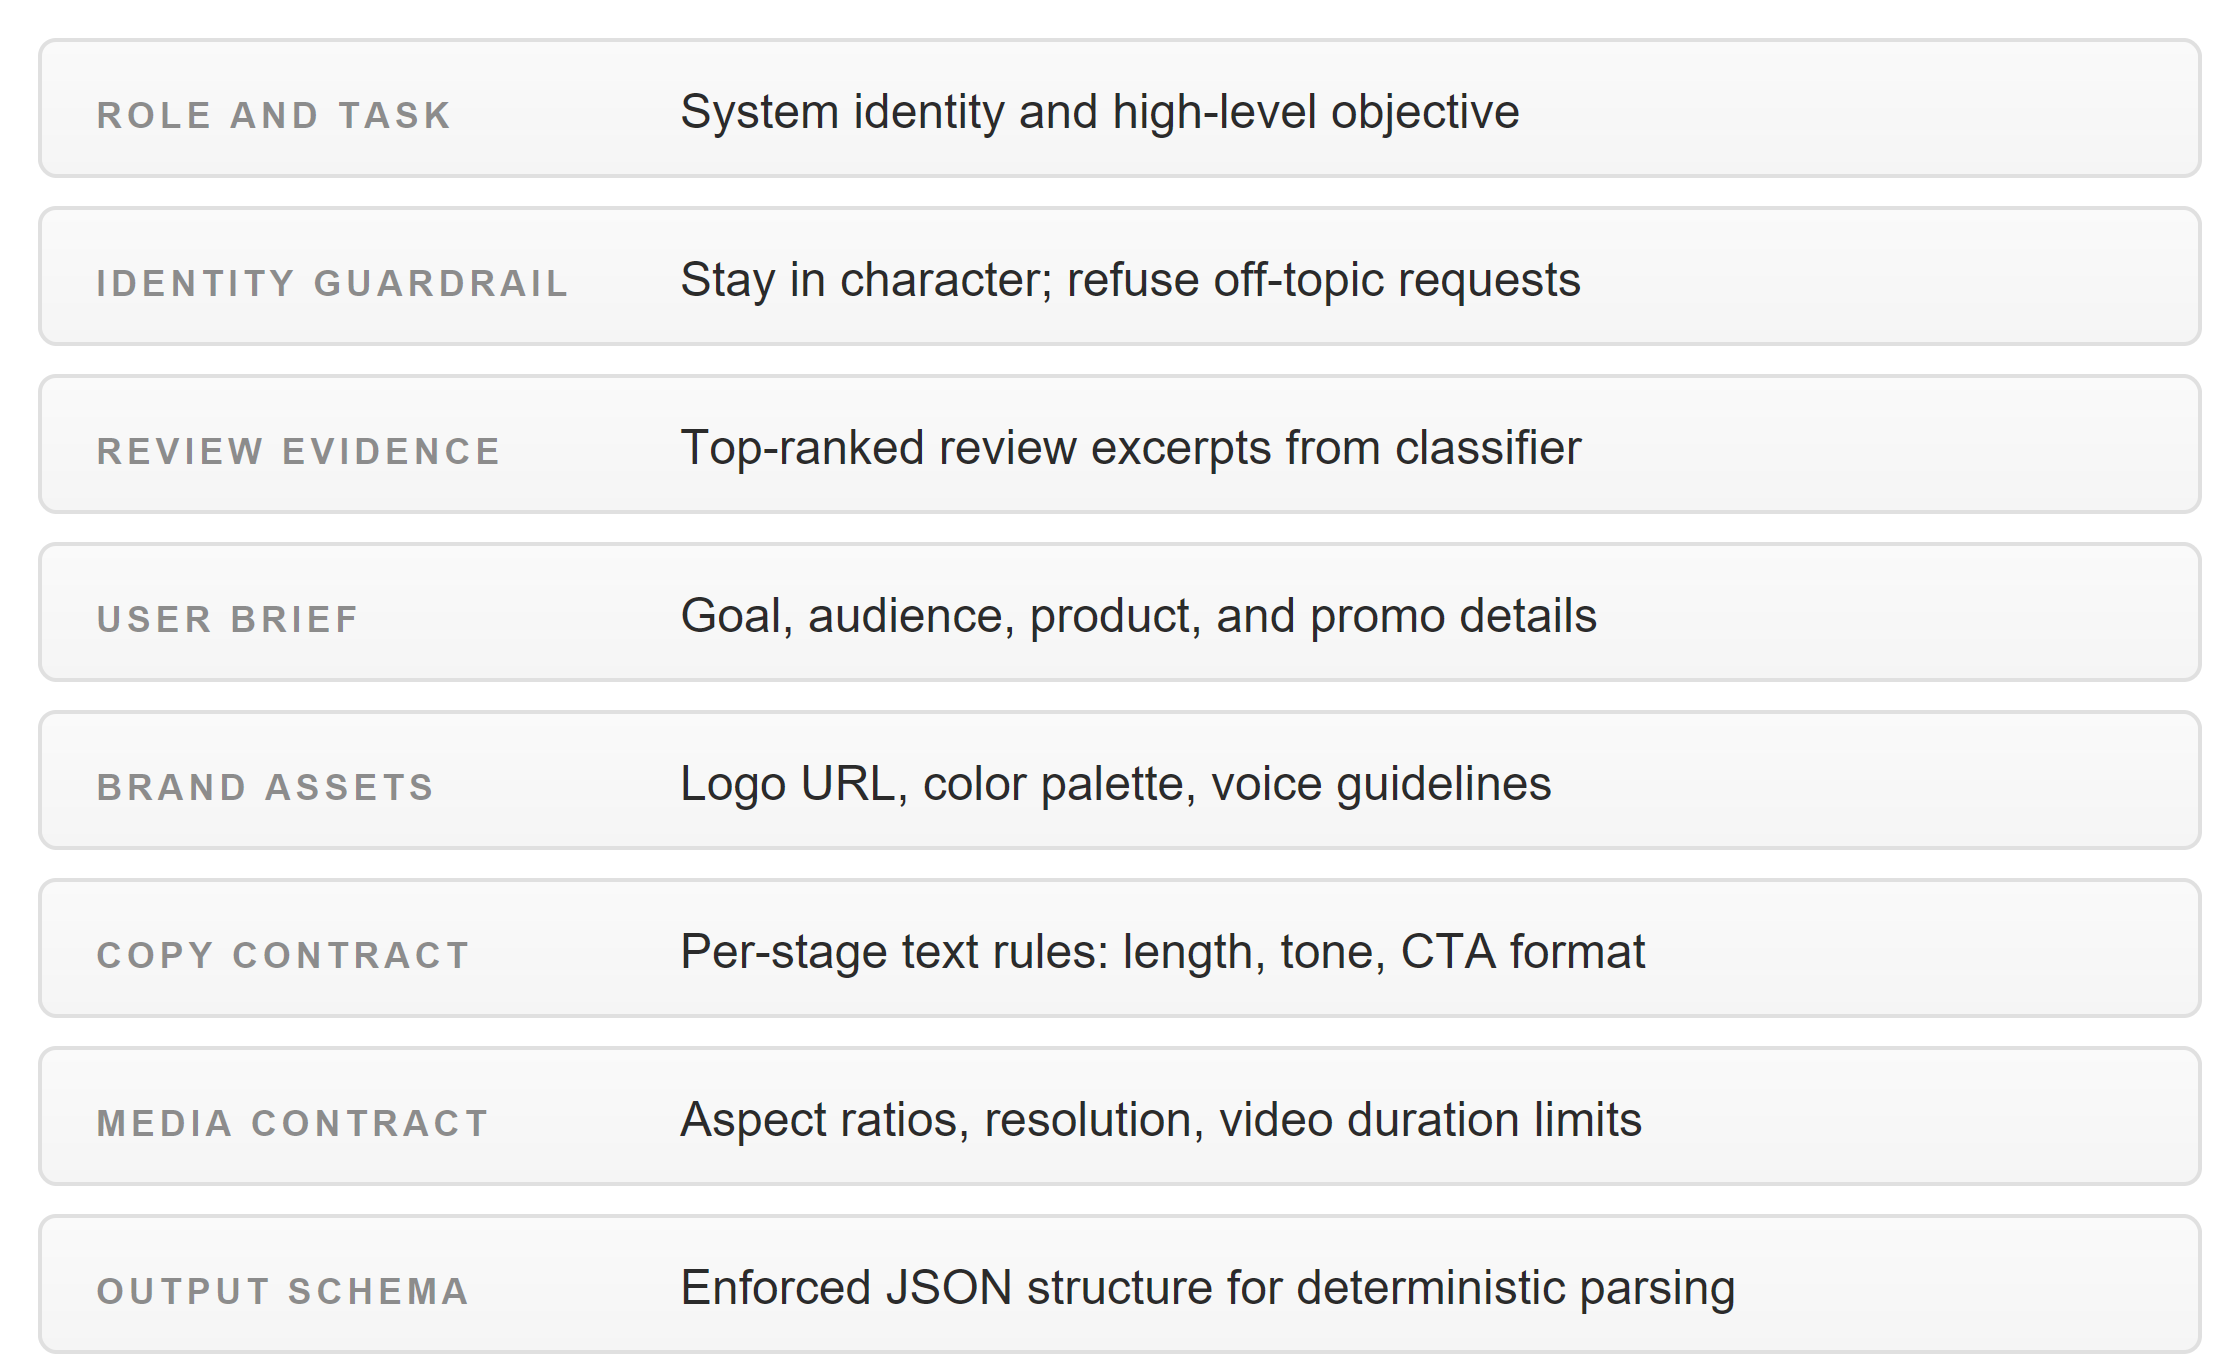
\includegraphics[width=\textwidth]{prompt-anatomy}
  \caption{Each block has one job. The model sees them in order and fills in the output schema.}
  \label{fig:prompt}
\end{figure}

One detail of the call architecture matters. Each campaign covers three funnel stages: an upper-funnel awareness or engagement stage, a middle-funnel consideration stage, and a lower-funnel sales stage. The system makes one model call per stage, not one monolithic call for the whole campaign. Splitting the call by stage keeps each request focused on a single funnel intent and keeps the output predictable. Inside each stage, the model produces three to five creative blocks, with a 9:16 short video as the hero block and 4:5 portrait static images for the rest.

Each creative block has two distinct copy surfaces. The first is the on-post text rendered onto the image: a short headline, a primary line, and a CTA, written under tight punctuation rules so they read cleanly inside the visual. The second is a paste-into-Meta caption: the full text the user pastes into the ad platform, which can be longer and use punctuation normally. Treating these as two surfaces avoids the common failure mode of generating one block of copy that fits neither place well. \Cref{fig:metablock-meta} in \cref{sec:metamapping} shows the ad-level Meta surface where the paste-into-Meta caption and its headline land.

The image, logo, concept-product, brand-guideline, and refinement prompts use the same pattern, but with narrower jobs. The static-image prompt prioritizes the uploaded product image, then the brand-guidelines PDF, then the logo, then free-text brand notes. The logo prompt is deliberately narrow: one flat 2D mark on a white background. The concept-product prompt creates a square concept render from the user's product idea and can reuse an uploaded logo. The refinement prompt edits only one creative block and keeps the strategy, audience, and budget locked. \Cref{app:prompts} gives the longer anatomy blocks for these prompts.

\subsection{Brand inputs, targeting, and visual generation}
\label{sec:brand}

The remaining runtime steps reuse machinery already described, so they are kept brief here; \cref{sec:web} shows them in the running application. The brand panel collects whatever assets the seller has: a logo (uploaded, or made with a narrow in-app generator that produces a flat 2D mark on a white background), a product image, a brand-guidelines PDF parsed for fonts and colours, and free-text notes. Sellers with only an idea can use concept-product mode\label{sec:concept}, which places the chosen or generated logo onto rendered packaging so an early-stage seller does not need real photography first. Optional price and sale fields drive promo badges on the visuals; when they are blank the platform never invents a number, a rule enforced inside the visual prompt rather than only at the interface.

Targeting and budget follow from the brief. The campaign goal (engagement, traffic, or sales) maps to a three-stage funnel, an upper-funnel awareness or engagement stage, a middle-funnel consideration stage, and a lower-funnel sales stage that is locked to a sales objective by design. The seller enters one total budget and the language model returns the percentage split across the three stages and across the blocks inside each stage. Each stage then carries its visuals: one 9:16 visual-only video (8 seconds) as the hero asset and several 4:5 portrait static images, produced by current image and short-video models. The brand inputs are carried into those visual prompts as a logo-placement rule, a colour palette, and a font instruction, and the on-image text from the structured prompt (\cref{sec:structured}) is rendered onto the statics by the image model itself.

\section{The web application}
\label{sec:web}

The web application is where the offline review intelligence and the runtime generation pipeline become usable by a non-technical seller. This section covers the application from two angles: the user journey that a seller walks through on the screen (\cref{sec:webjourney}) and the engineering implementation underneath it (\cref{sec:webapp}). The two views are companions, not alternatives.

\begin{figure}[ht!]
  \centering
  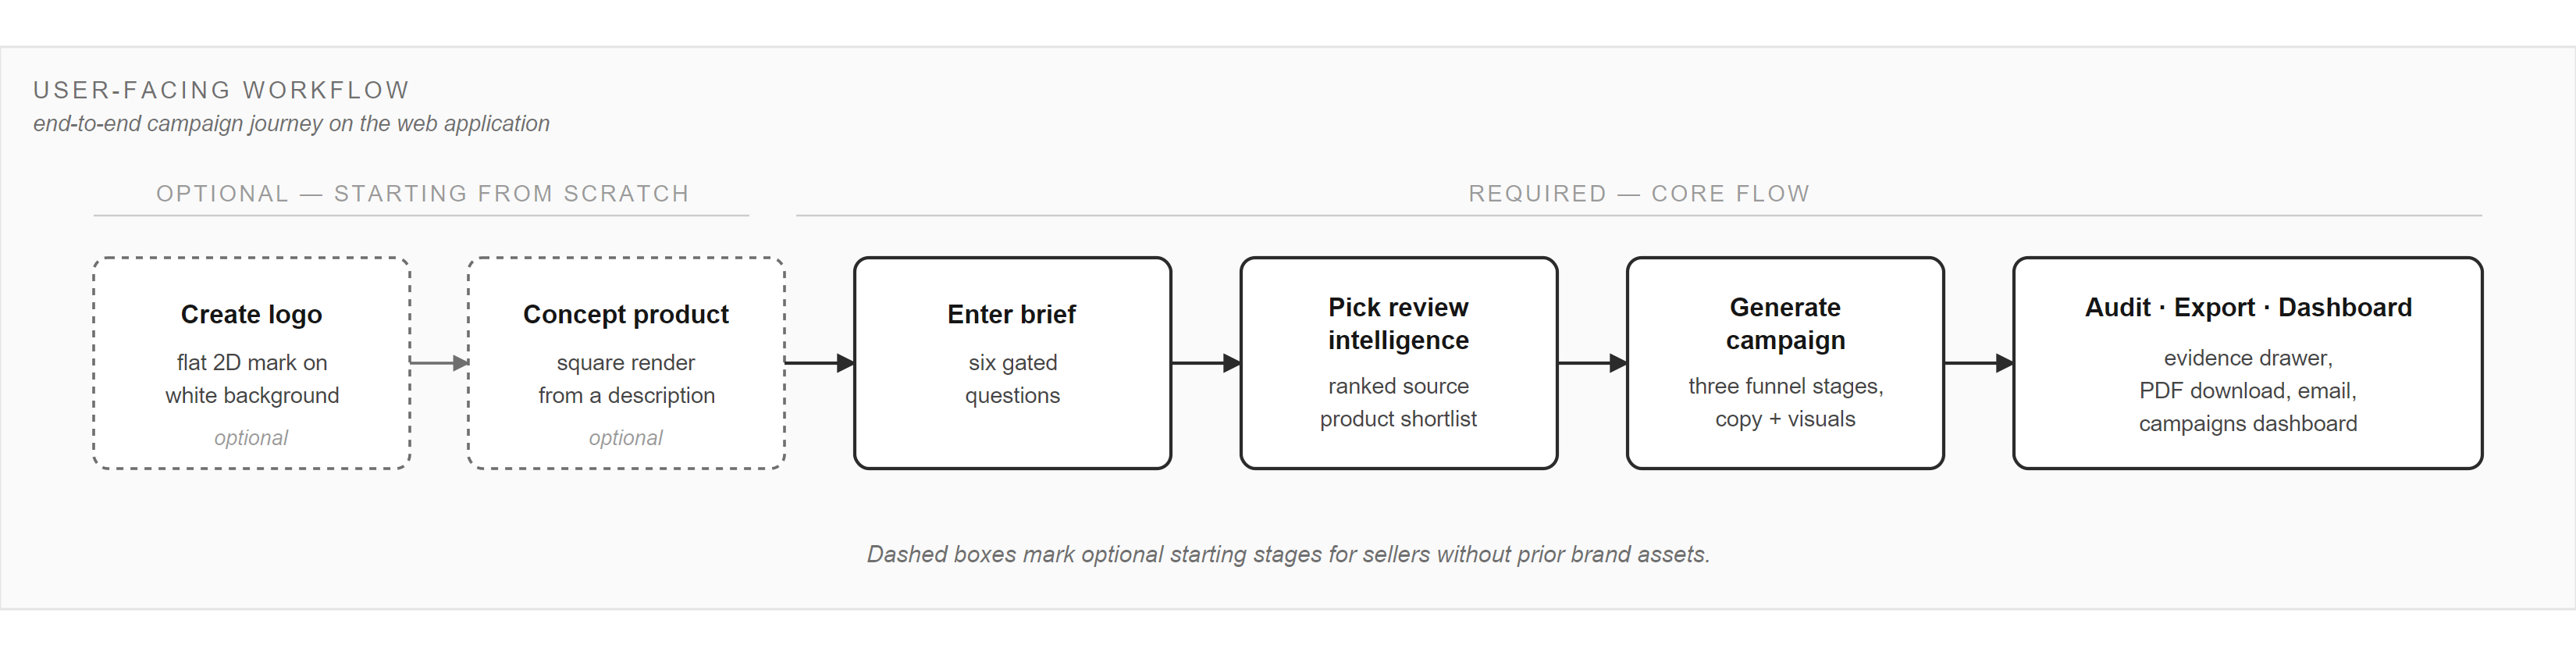
\includegraphics[width=\textwidth]{round5-user-workflow}
  \caption{End-to-end user journey on the MarketMind web application. The two dashed stages on the left are optional starting points for sellers without prior brand assets; the four solid stages from the brief onward are the core flow every campaign runs through.}
  \label{fig:userworkflow}
\end{figure}

\Cref{fig:userworkflow} is a user-facing companion to the technical architecture in \cref{fig:architecture}. The architecture diagram shows where the data sits and which model produces what; the user journey shows what a seller does in front of the screen.

\subsection{User journey}
\label{sec:webjourney}

This subsection walks through what a user actually does on each screen of the application, from a starting point of no brand assets to a delivered campaign report.

\subsubsection{Logo and product concept (optional starting stages)}
\label{sec:userlogo}

The two stages on the left of \cref{fig:userworkflow} are skipped by any seller who already has a brand identity and a real product photo. They are there for a different audience. A new e-commerce seller may have located a supplier or manufacturer for a product idea, intends to buy in bulk and resell online, and has not yet committed to a logo, a packaging style, or a product photograph that they could upload as a reference. The application provides two compact tools for that case.

The logo generator (\cref{fig:logogen}) renders a flat 2D mark on a clean white background from a brand name, a palette description in plain English, an optional visual element, and one geometry preset plus one theme preset. The geometry presets are wordmark, circle badge, angular mark, and rounded icon; the theme presets are modern, outdoor, luxury, playful, rustic, and tech. The output is bounded and repeatable rather than free-form, which keeps the demonstration honest about its scope: the generator produces a usable mark in seconds, not a hand-crafted brand identity.

\begin{figure}[ht!]
  \centering
  
\includegraphics[width=\textwidth]{fig-logo-generator}
  \caption{In-app logo generator. The user fills brand name and palette, optionally picks a visual element chip, then chooses one geometry preset and one theme preset. The generated mark renders on a clean white background.}
  \label{fig:logogen}
\end{figure}

The product-concept tool renders a square hero shot of the product from a short text description, and can place a generated or uploaded logo on the rendered packaging. \Cref{fig:concept} shows the modal. The framing is honest: the output is a concept render that the seller can use to anchor a campaign visually before any manufactured artwork exists.

\begin{figure}[ht!]
  \centering
  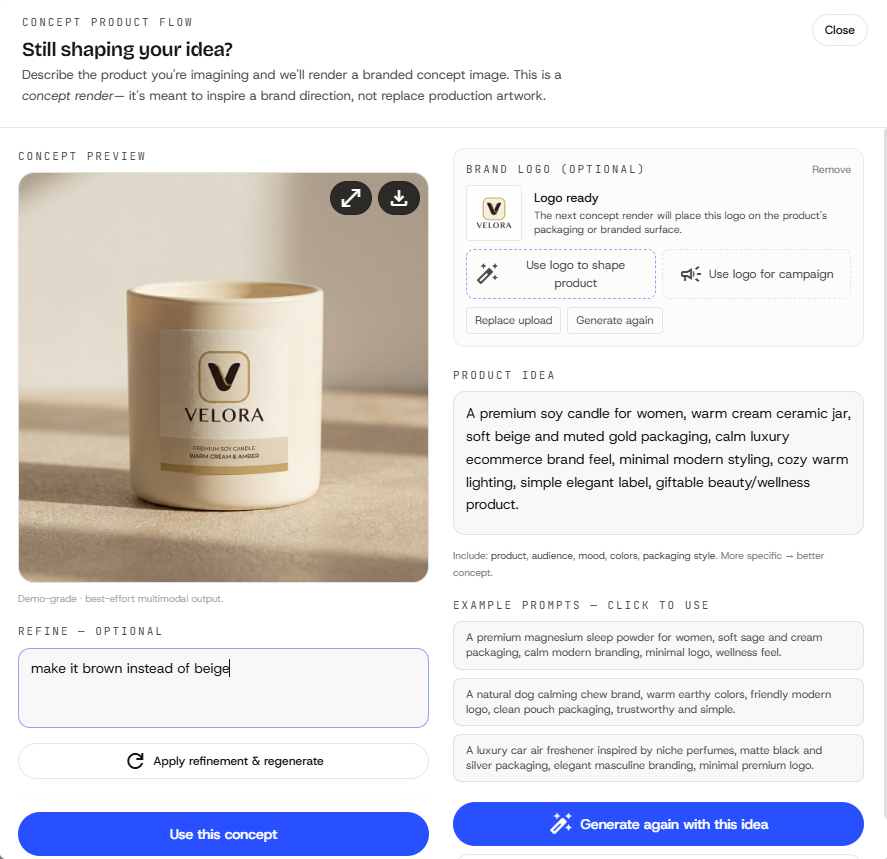
\includegraphics[width=\textwidth]{fig-product-concept}
  \caption{Concept-product render modal. The user provides a short description of the product idea, optionally attaches a previously generated logo, and the system returns a square concept image that can act as the visual anchor for the campaign when no real product photo is available.}
  \label{fig:concept}
\end{figure}

Both stages are concept support, not final manufacturing artwork. A seller who already has a real product photo or a hand-drawn logo can skip both and upload those assets later, on the Campaign Output screen described in \cref{sec:usercampaign}.

\subsubsection{Brief: the six questions}
\label{sec:userbrief}

After the optional logo and product-concept stages, the Brief is a six-step gated form that captures the minimum a small seller needs to specify before a review-grounded campaign plan can be built. The user cannot skip ahead. \Cref{fig:brief6} shows the six questions in one composite frame.

\begin{figure}[ht!]
  \centering
  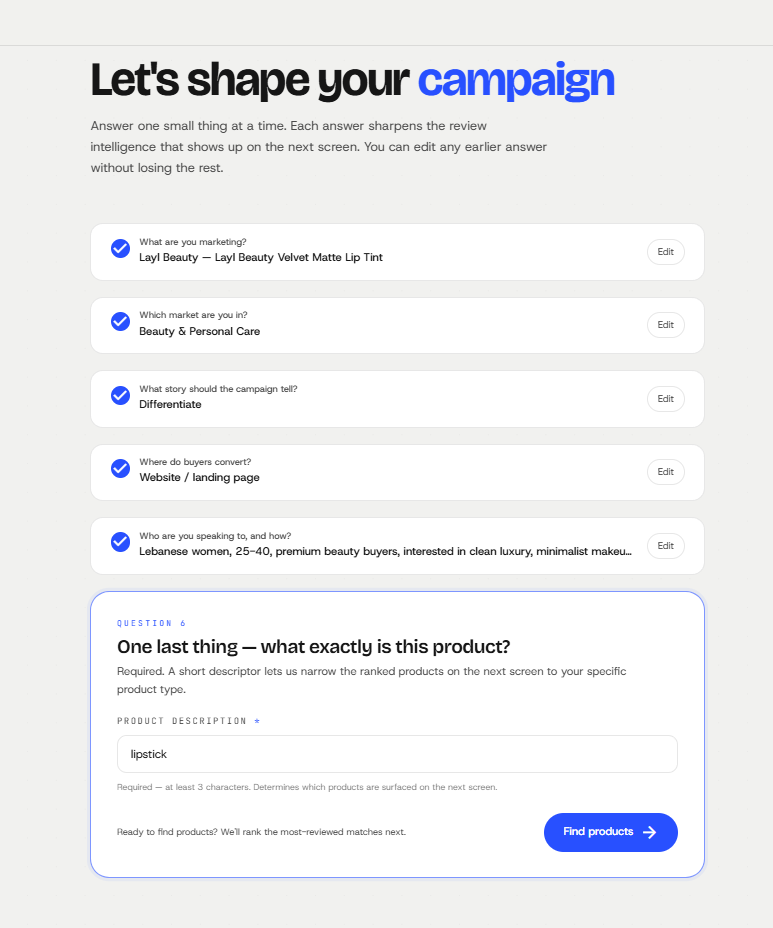
\includegraphics[width=\textwidth]{brief-6-questions}
  \caption{The six gated questions on the Brief screen, shown end-to-end in a single composite frame. Each question commits its answer to the working draft only on advance, and the user can return to any earlier question without losing the rest.}
  \label{fig:brief6}
\end{figure}

The six inputs map directly to the structured prompt that the language model reads on every funnel stage.

\textbf{Brand name and product name.} These anchor the campaign identity across the report, the dashboard, and the generated copy. They are kept distinct from the review-intelligence source product name; the source product is the body of customer language the model reads, not the campaign's brand.

\textbf{Category.} Ten broad Amazon categories are supported: Baby Products, Beauty and Personal Care, Electronics, Health and Household, Home and Kitchen, Office Products, Pet Supplies, Sports and Outdoors, Tools and Home Improvement, and Toys and Games. The category selects which slice of the offline review intelligence the goal-aware ranking layer searches.

\textbf{Campaign goal.} Three goals are supported: highlight strengths, address objections, and differentiate. The goal drives which of the three ranking formulas fires in the goal-aware ranking layer described in \cref{sec:ranking}.

\textbf{Business model.} Website, WhatsApp, app, or in-person. The business model changes the call-to-action verbs in the generated copy so the prompt does not produce a Shop Now CTA for a WhatsApp business.

\textbf{Audience and tones.} A short audience description plus one or more tone chips. The audience and tones feed the structured prompt's targeting block and shape the messaging angle.

\textbf{Product description.} A free-text paragraph describing the product. This adds practical context that the review intelligence cannot supply on its own, such as supplier constraints, regional positioning, or known limitations.

The six inputs are not optional. They are the floor needed to ground generation in something specific rather than generic. The brief commits as a single draft row only on final submit; downstream screens then patch the same row as the user picks a product, fills the brand panel, and generates each stage.

\subsubsection{Product intelligence display}
\label{sec:userintel}

Once the brief is submitted, the Product Intelligence screen returns a ranked shortlist of similar products under the chosen campaign goal, drawn from the per-product profiles produced offline. The user picks one product as the evidence source for the campaign. The picked product is not treated as the campaign's identity, only as the body of customer language the structured prompt reads at generation time.

The screen exposes the per-product evidence profile so the user can decide on the strength of the evidence before committing. \Cref{fig:productintel} and \cref{fig:productintel2} show two different products and two different evidence profiles.

\begin{figure}[ht!]
  \centering
  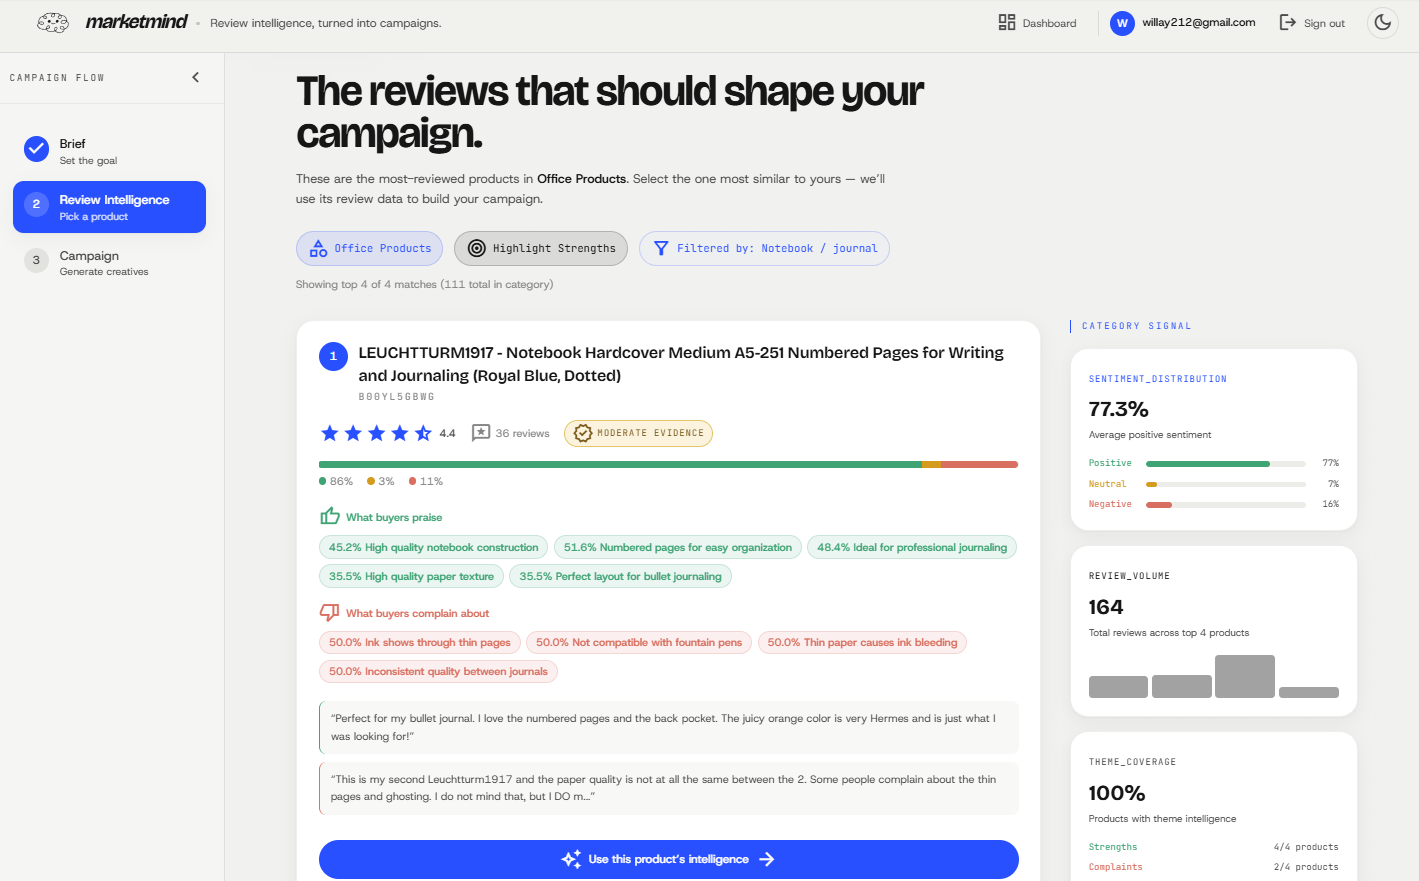
\includegraphics[width=\textwidth]{fig-product-intelligence}
  \caption{Product Intelligence screen for the Velvet Matte Lip Tint campaign. The card shows the source product (Revlon Super Lustrous Lipstick), the review count, the positive/neutral/negative sentiment split, the extracted strengths and complaints, and a curated set of review excerpts.}
  \label{fig:productintel}
\end{figure}

\begin{figure}[ht!]
  \centering
  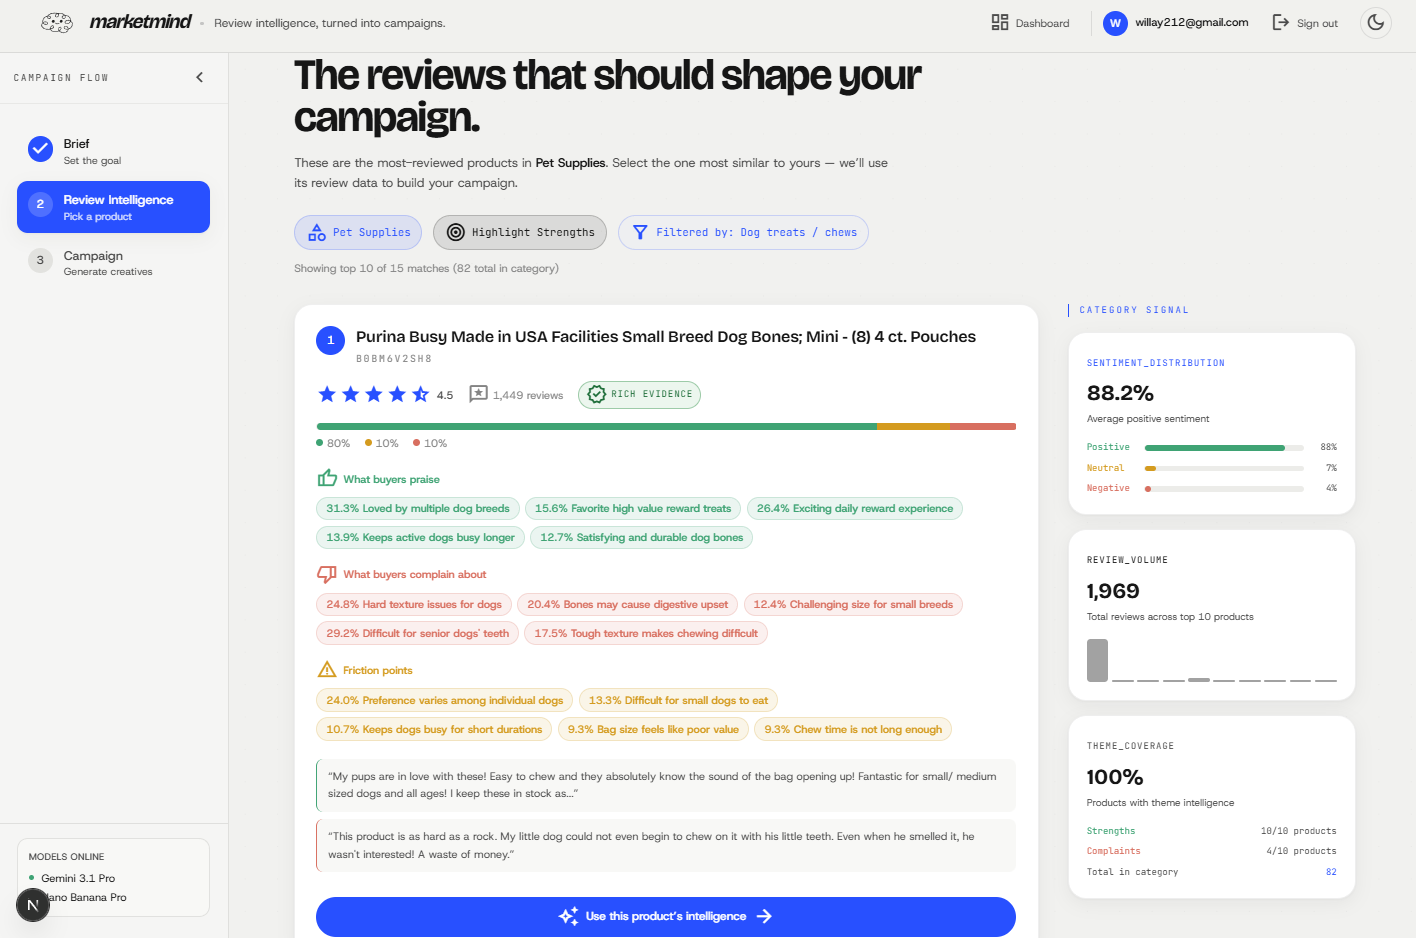
\includegraphics[width=\textwidth]{fig-product-intelligence-2}
  \caption{A second Product Intelligence view on a different campaign, showing a different evidence profile. The same screen surface adapts to whatever pattern the source product's review corpus actually carries.}
  \label{fig:productintel2}
\end{figure}

The reader should notice five things on each card. The review count tells the user how much evidence is behind the campaign. The positive, neutral, and negative split tells the user what kind of campaign they can plausibly run on this product: an objection-handling campaign will not work on a product whose reviews are 95\,\% positive with only a handful of complaints. The extracted strengths and complaints give the structured prompt the messaging angles it will consider. The friction points name specific buyer concerns where they exist. The review excerpts give the model the customer language it will draw on for the on-image copy.

Some products show mainly positive evidence because that is what the source corpus contains. Other products show a richer profile with friction points and neutral excerpts. The screen does not invent variety: when a corpus is light on negative or neutral reviews, a limited-evidence badge surfaces that fact rather than fabricating coverage. The Round 4 ablation in \cref{sec:ablation} reports four such cases across four categories.

\subsubsection{Campaign generation}
\label{sec:usercampaign}

The Campaign Output screen opens with the brand panel\label{sec:userbrand}, the user's single intake surface for the assets that condition the downstream prompts. The panel is shown in \cref{fig:brandpanel}. It collects four optional asset slots and a budget block: a product image, a brand-guidelines PDF, an uploaded or in-app generated logo, a free-text brand context, a total budget, and an optional promo block (currency, price, sale percentage).

\begin{figure}[ht!]
  \centering
  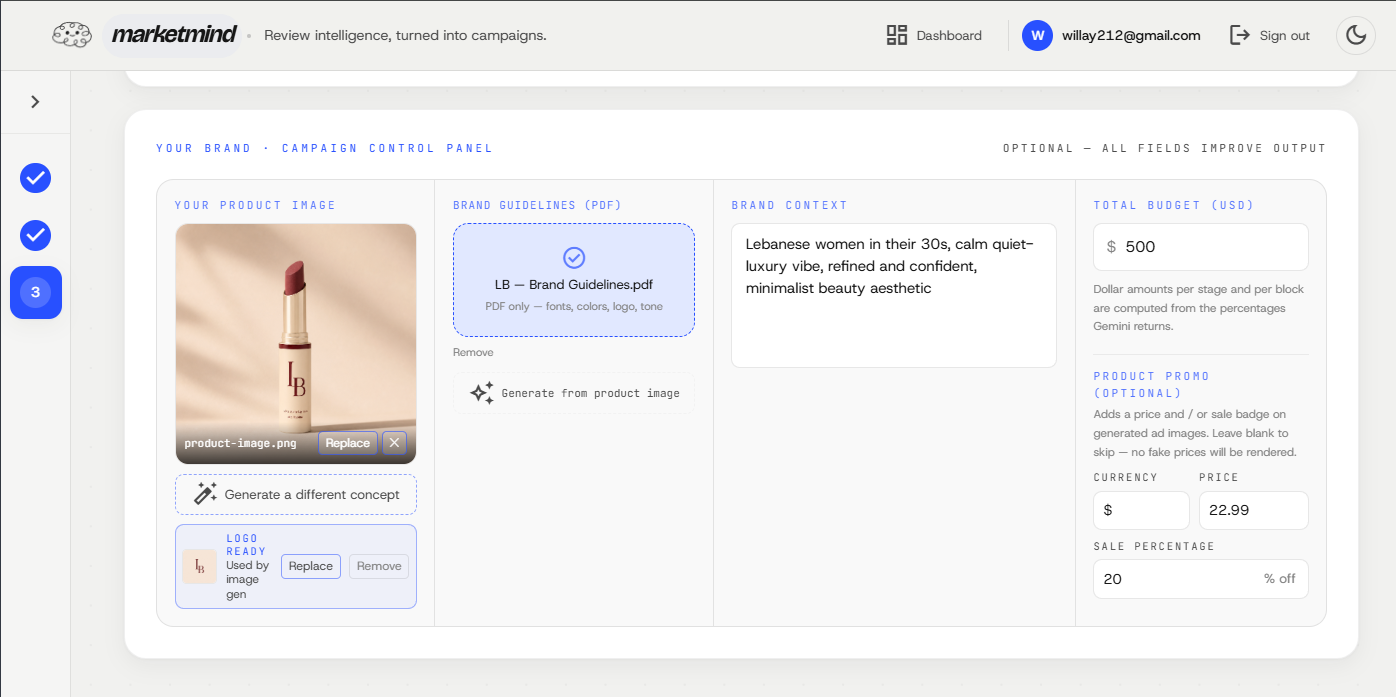
\includegraphics[width=\textwidth]{fig-brand-panel}
  \caption{Brand asset intake on the Campaign Output screen. The single panel collects the product image, logo, brand-guidelines PDF, free-text brand context, total budget, and optional promo (currency, price, sale percentage) that the downstream prompts read at generation time.}
  \label{fig:brandpanel}
\end{figure}

Each slot has a defined role in the downstream prompts. The product image is the source of truth for what the product looks like; the structured image prompt prioritises it over the rest of the references for product appearance. The brand-guidelines PDF supplies palette and typography. The logo carries the brand mark and is placed visibly on the rendered creatives. The free-text brand context informs tone, voice, and whether the visual concept features a person or audience type. The promo fields drive the on-image price and discount badges; when both fields are empty the platform never invents a number. The honest framing in \cref{sec:webscope} applies here: brand consistency in the rendered visuals is bounded by the prompt-following fidelity of the image model. The panel cannot enforce style at the model level; it can only structure the inputs the model reads.

Once the panel is set and the user picks the source product, the Campaign Output screen renders the three funnel stages of a Meta-style campaign. Each stage carries a 9:16 short video (visual-only) as the hero asset, several 4:5 portrait static creatives with on-image copy, the paste-into-Meta caption, the budget split, the messaging angle, the audience direction, and the visual concept. The implementation of this generation step lives in \cref{sec:webapp} and the structured prompt that drives it is described in \cref{sec:structured}; the focus here is on what the user sees and does.

The user can refine any individual block without retriggering the whole stage. Refinement is gated to the editable surfaces: the two copy surfaces, the design direction, the visual concept, and the motion direction for video blocks. Strategy, audience, interests, and budgets stay locked, so a refinement run never quietly changes the campaign's planning layer.

\subsubsection{Meta Ads implementation mapping}
\label{sec:metamapping}

\begin{wrapfigure}{r}{0.42\textwidth}
  \centering
  \vspace{-0.4em}
  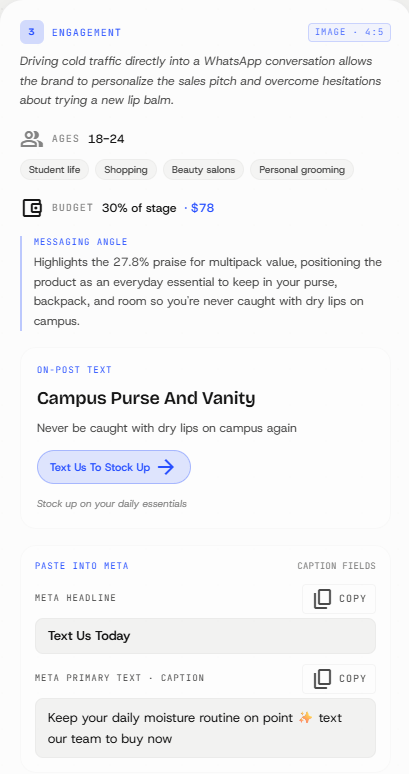
\includegraphics[width=0.4\textwidth]{fig-meta-block-mm}
  \caption{One creative block as MarketMind renders it. The structured fields the user later pastes into Meta Ads Manager sit alongside the creative itself: campaign objective, audience description with age range and detailed-targeting interests, daily budget for the stage, messaging angle, and the on-image copy and paste-into-Meta caption.}
  \label{fig:metablock}
\end{wrapfigure}

MarketMind does not connect to Meta and does not launch ads through any Meta API. The platform outputs every field a seller needs to launch the campaign manually, in the same shape Meta asks for during the Ads Manager wizard. A user who runs their own ads on Meta faces a fixed set of fields at campaign-, ad-set-, and ad-level: a campaign objective, an audience description, an age range, a list of detailed-targeting interests, a daily budget, and a creative file with its caption and its headline. MarketMind renders every one of those values inside each creative block. \Cref{fig:metablock} on the right shows one such block. The user opens Meta Ads Manager, walks the funnel-stage wizard, and pastes the values from the report into the matching fields. \Cref{fig:metablock-meta} shows the four Meta surfaces a user would step through to launch the same campaign: the Engagement campaign objective at campaign level, the daily-budget setting at ad-set level, the audience and detailed-targeting page at ad-set level, and the ad-level surface with the uploaded creative and the caption and headline in place.

The Meta-style framing used throughout this report refers to the structural alignment of the output with the fields Meta asks for during the wizard flow, not to any integration with Meta's advertising platform. The seller copies each value from the report into Meta Ads Manager by hand, the same way they would copy a brief from a slide deck.

\begin{figure}[ht!]
  \centering
  \begin{subfigure}[t]{0.48\textwidth}
    \centering
    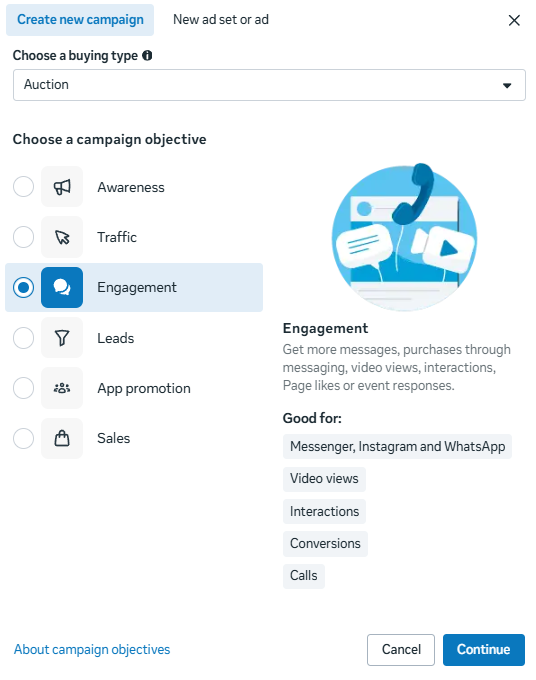
\includegraphics[width=\textwidth]{fig-meta-block-meta-1}
    \caption{Meta Ads Manager, campaign level: \textit{Engagement} chosen as the campaign objective.}
    \label{fig:metablock-meta-a}
  \end{subfigure}
  \hfill
  \begin{subfigure}[t]{0.48\textwidth}
    \centering
    
\includegraphics[width=\textwidth]{fig-meta-block-meta-2}
    \caption{Meta Ads Manager, ad-set level: the daily-budget field for the stage.}
    \label{fig:metablock-meta-b}
  \end{subfigure}

  \vspace{0.6em}

  \begin{subfigure}[t]{0.48\textwidth}
    \centering
    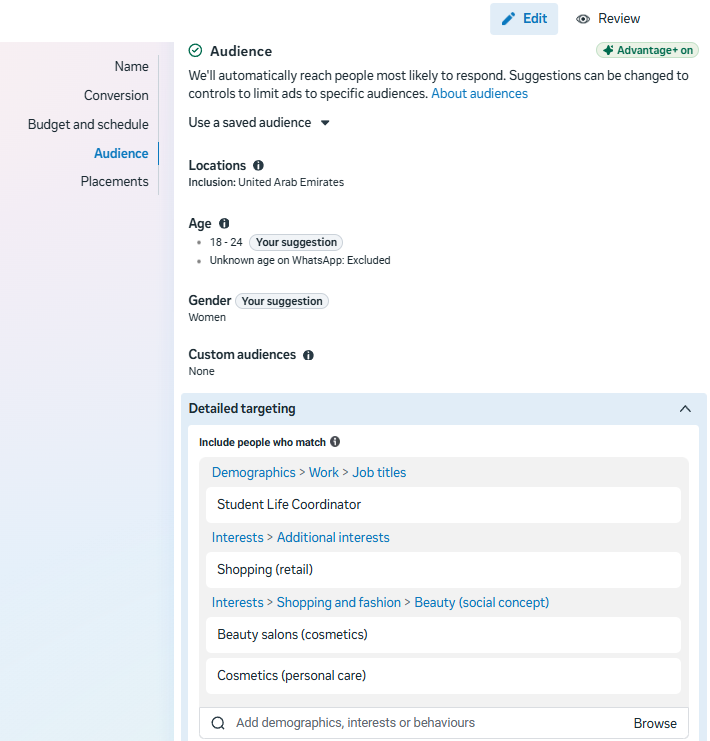
\includegraphics[width=\textwidth]{fig-meta-block-meta-3}
    \caption{Meta Ads Manager, ad-set level: the age range and the detailed-targeting interest list.}
    \label{fig:metablock-meta-c}
  \end{subfigure}
  \hfill
  \begin{subfigure}[t]{0.48\textwidth}
    \centering
    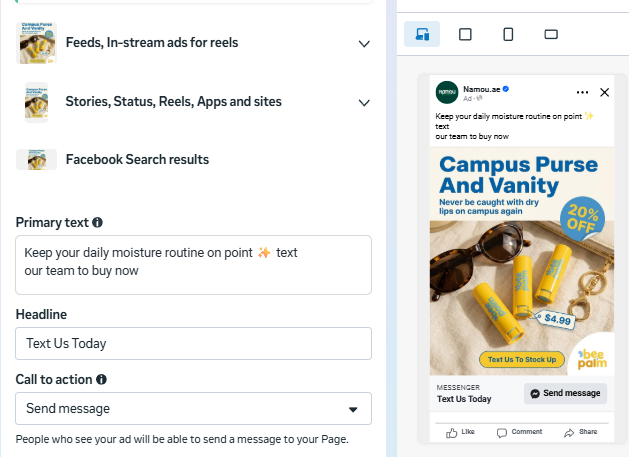
\includegraphics[width=\textwidth]{fig-meta-block-meta-4}
    \caption{Meta Ads Manager, ad level: the rendered creative uploaded, with the on-image copy baked into the visual and the paste-into-Meta caption and headline filled into the text fields.}
    \label{fig:metablock-meta-d}
  \end{subfigure}
  \caption{The four Meta Ads Manager surfaces a user would step through to launch the campaign that \cref{fig:metablock} planned. MarketMind does not connect to the Meta API; the user pastes each value into Meta Ads Manager by hand.}
  \label{fig:metablock-meta}
\end{figure}

\subsubsection{Evidence drawer}
\label{sec:webdrawer}

The evidence drawer is the part of the application that justifies calling the generation grounded rather than informed. Every creative block carries a small button that opens a panel with the review excerpts that the structured prompt fed the model when it produced that block. The drawer shows the positive, neutral, and negative excerpts the model saw, the per-product sentiment profile that the goal-aware ranking layer used to pick the source product, and the brand-context inputs (logo, product image, brand-guidelines PDF, free-text notes) that fed the prompt. A user, a reviewer, or a jury member can therefore audit any line of generated copy or any design choice back to the customer language and the brand asset that produced it. The drawer is shown in \cref{fig:evidencedrawer} on the cosmetics campaign and in \cref{fig:evidencedrawer2} on a pet-supplies campaign, showing that the same evidence pattern carries across product categories.

\begin{figure}[ht!]
  \centering
  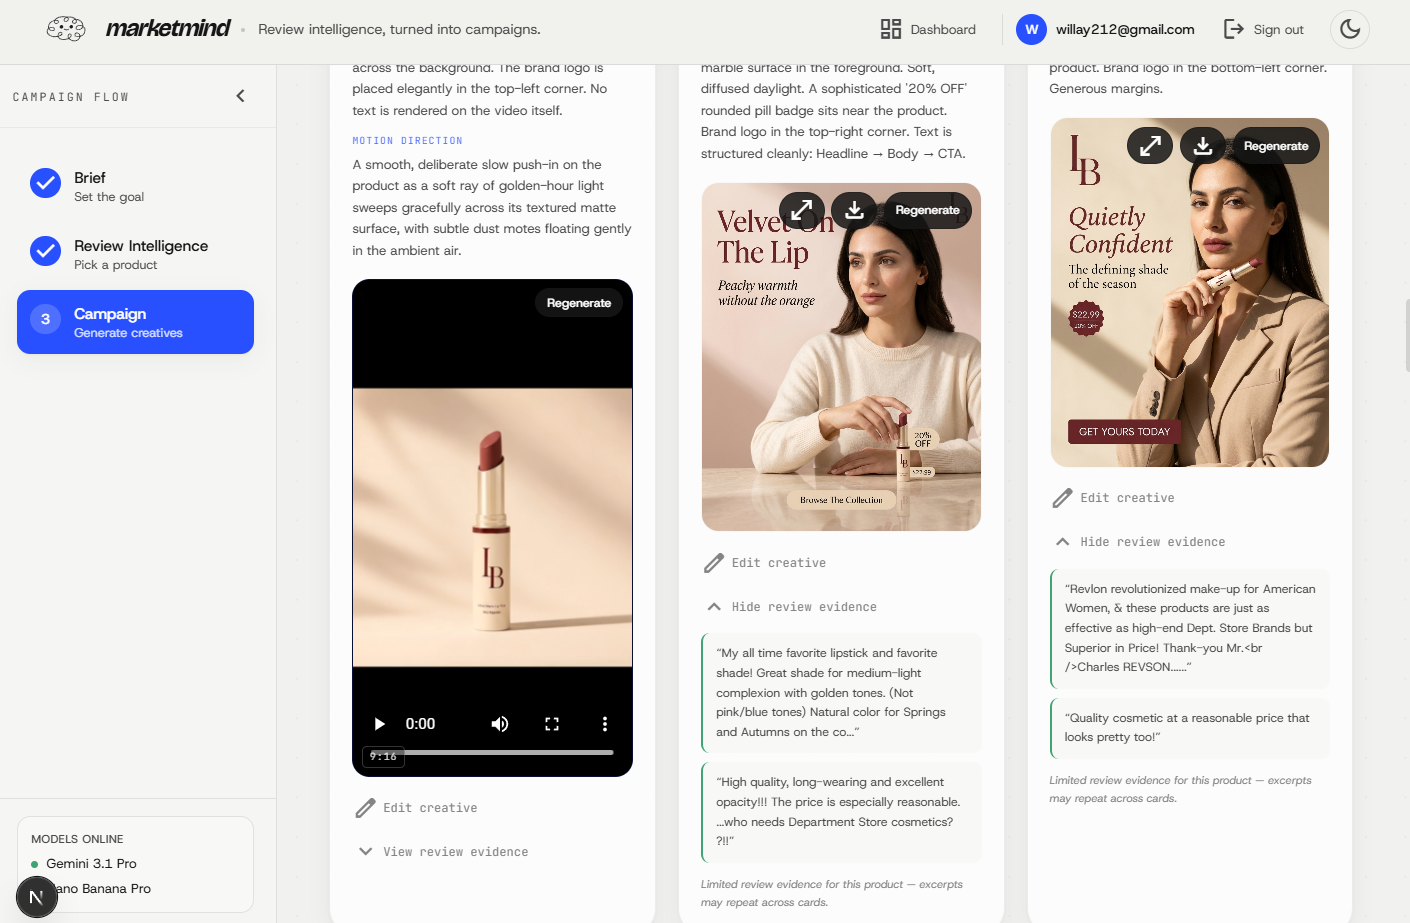
\includegraphics[width=\textwidth]{fig-evidence-drawer}
  \caption{The evidence drawer expanded under one creative block on the Campaign Output screen for the cosmetics campaign \textit{Velvet Matte Lip Tint}. The drawer surfaces the review excerpts the model saw at generation time, so every generated line can be read against the customer language that produced it.}
  \label{fig:evidencedrawer}
\end{figure}

\begin{figure}[ht!]
  \centering
  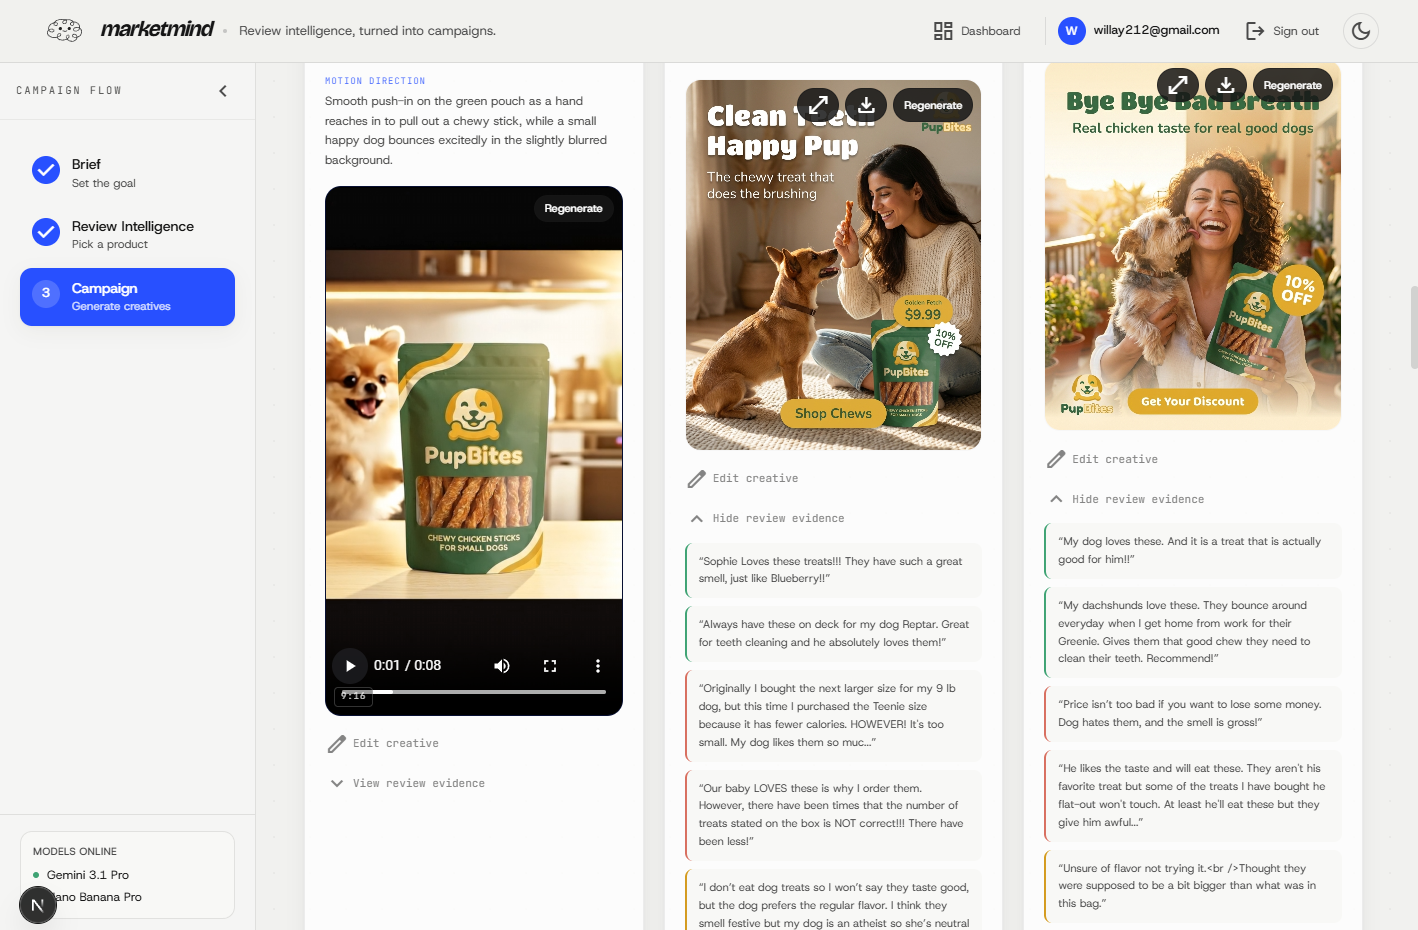
\includegraphics[width=\textwidth]{fig-evidence-drawer-2}
  \caption{A second evidence-drawer view, on the pet-supplies campaign \textit{PupBites}. Real review excerpts about the source dog-treat product sit directly beneath the creative block they grounded, available to the user at audit time without leaving the campaign screen.}
  \label{fig:evidencedrawer2}
\end{figure}

\subsubsection{Report export and email delivery}
\label{sec:webexport}

The campaign view is exported as a single PDF rendered on the client through \texttt{html2canvas} and \texttt{jspdf}. The PDF carries a cover page with the user's brand and product name, one page per funnel stage with the generated visuals and copy, and a sanitiser pass that strips characters the embedded Helvetica cannot render (emojis, smart quotes, letter-spaced text). The on-image text and the paste-into-Meta caption are rendered as separate rows so the user can drop each one into the right field of the Meta ad composer without manual splitting. A preview of the rendered PDF is shown in \cref{fig:pdfexport}. The same campaign can be emailed directly to the user's inbox through \texttt{/api/send-email}, which calls Resend with a subject and body that lead with the campaign name.

\begin{figure}[ht!]
  \centering
  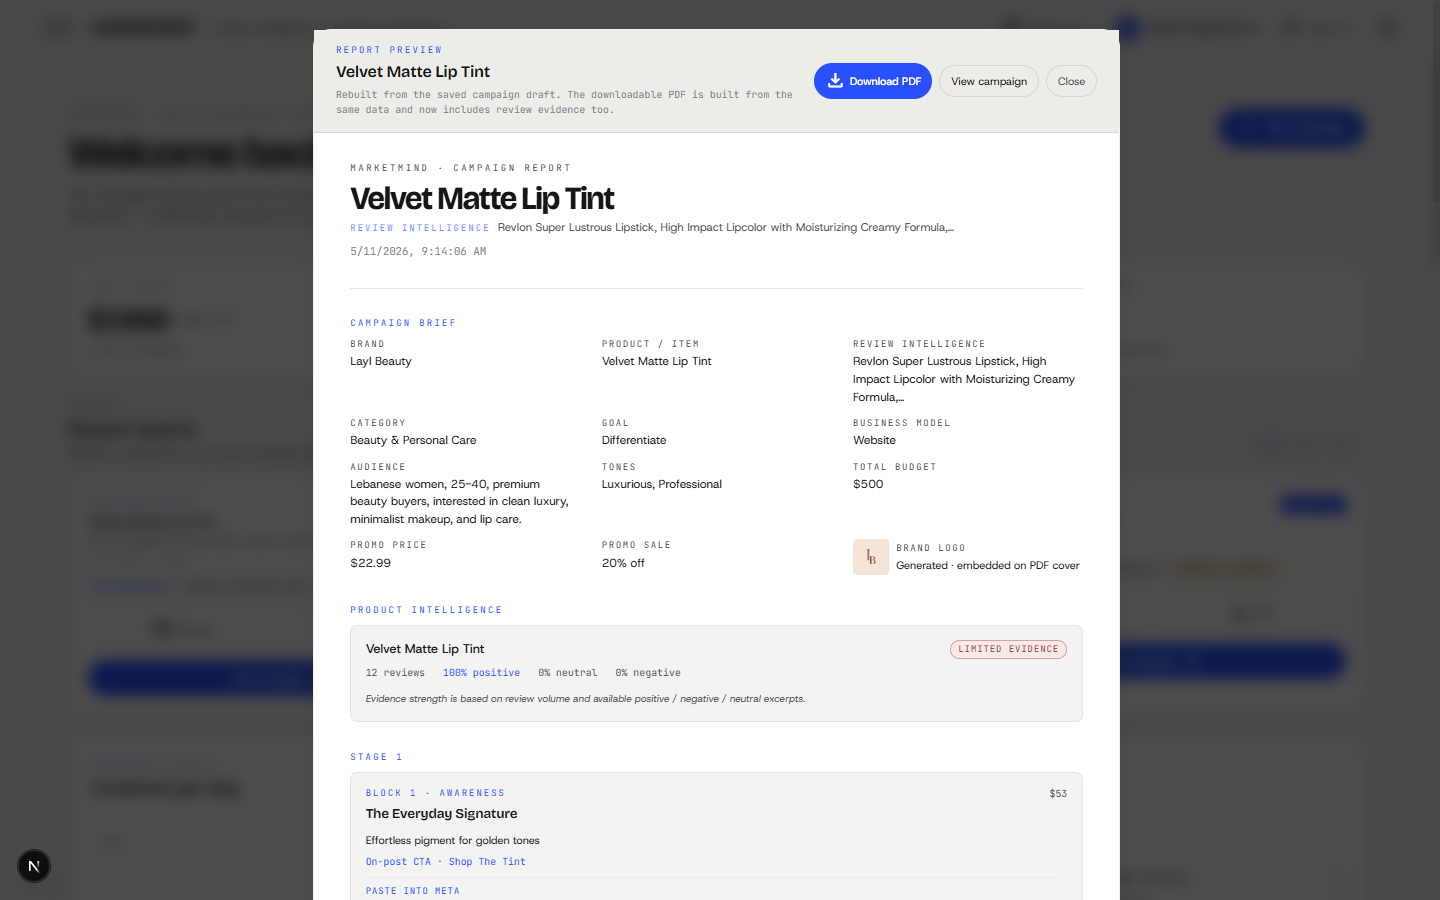
\includegraphics[width=\textwidth]{fig-pdf-export}
  \caption{Report preview modal on the Dashboard. The user-facing campaign name (\textit{Velvet Matte Lip Tint}) leads the report; the review-intelligence source product (\textit{Revlon Super Lustrous Lipstick}) renders as a secondary subheader, with the brief fields, brand identity, product-intelligence summary, and Stage 1 creative block below. Downloading the PDF renders this view client-side through \texttt{html2canvas} and \texttt{jspdf}.}
  \label{fig:pdfexport}
\end{figure}

\subsubsection{Dashboard}
\label{sec:userdash}

The Dashboard is the application's standing surface across sessions. It is where the user lands after sign-in and where they return after a campaign run. Three screenshots cover the dashboard's main blocks. \Cref{fig:dash1} shows the headline campaign counts and recent activity, \cref{fig:dash2} shows the campaigns and drafts grid, and \cref{fig:dash3} shows the report and product-intelligence history.

\begin{figure}[ht!]
  \centering
  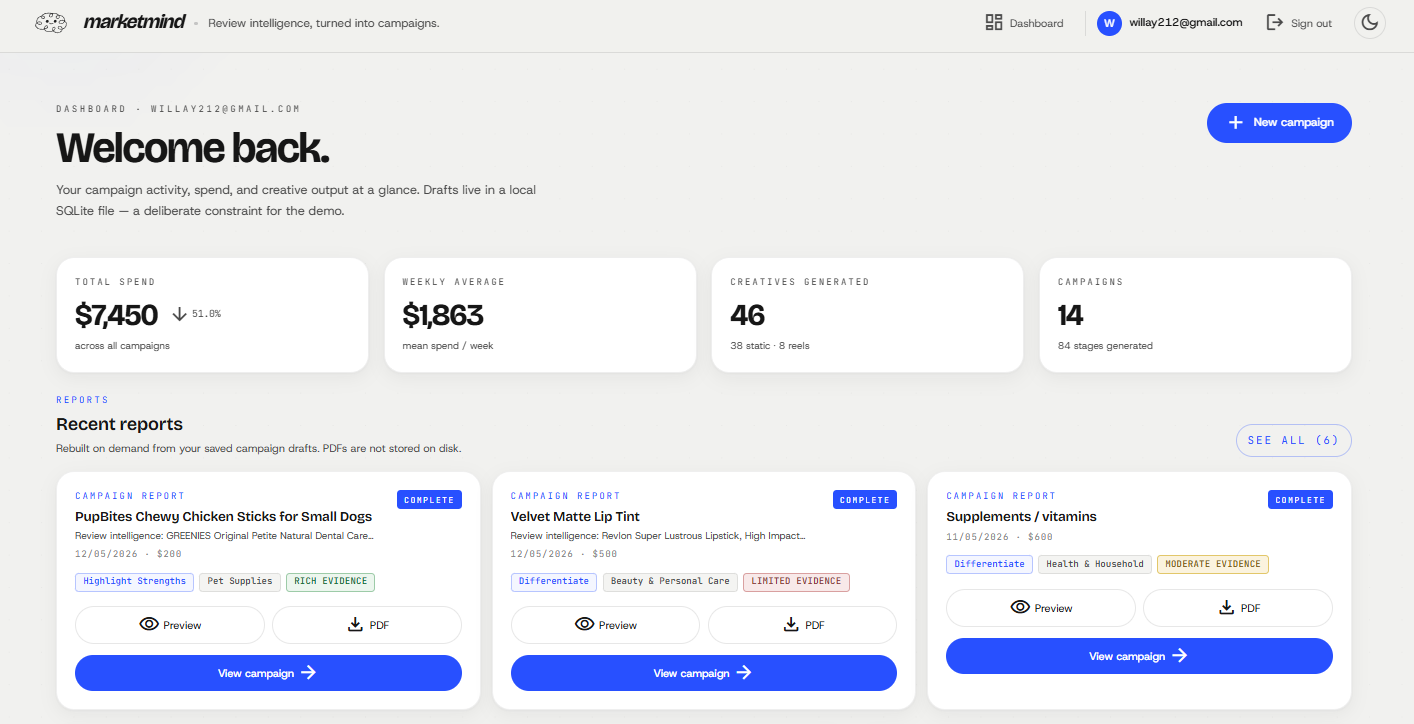
\includegraphics[width=\textwidth]{dash-1}
  \caption{Dashboard, top section. Headline campaign counts, budget totals, creative mix, and recent activity computed from the user's draft rows.}
  \label{fig:dash1}
\end{figure}

\begin{figure}[ht!]
  \centering
  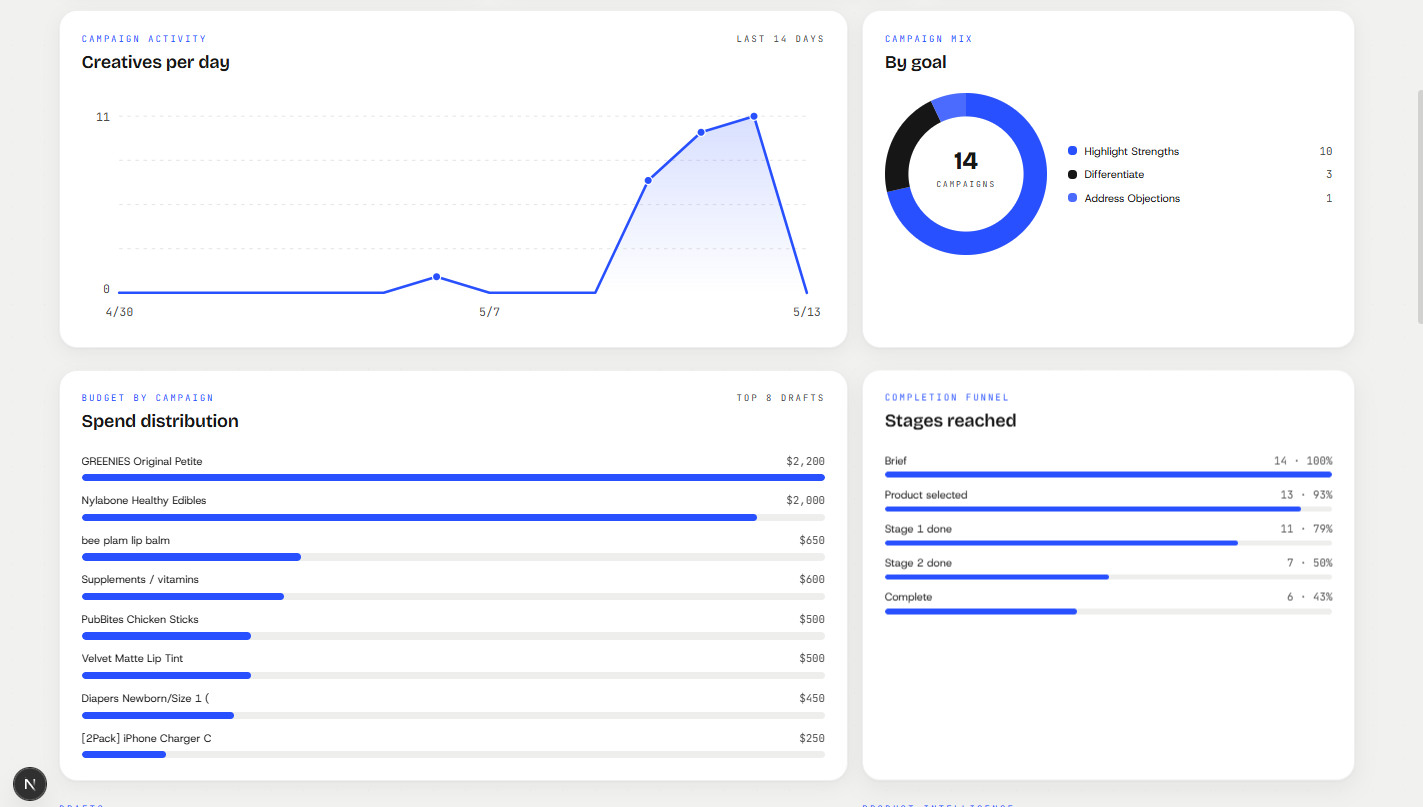
\includegraphics[width=\textwidth]{dash-2}
  \caption{Dashboard, campaigns and drafts. Each row is a campaign in progress or a completed campaign; the status field on the draft row drives the badge.}
  \label{fig:dash2}
\end{figure}

\begin{figure}[ht!]
  \centering
  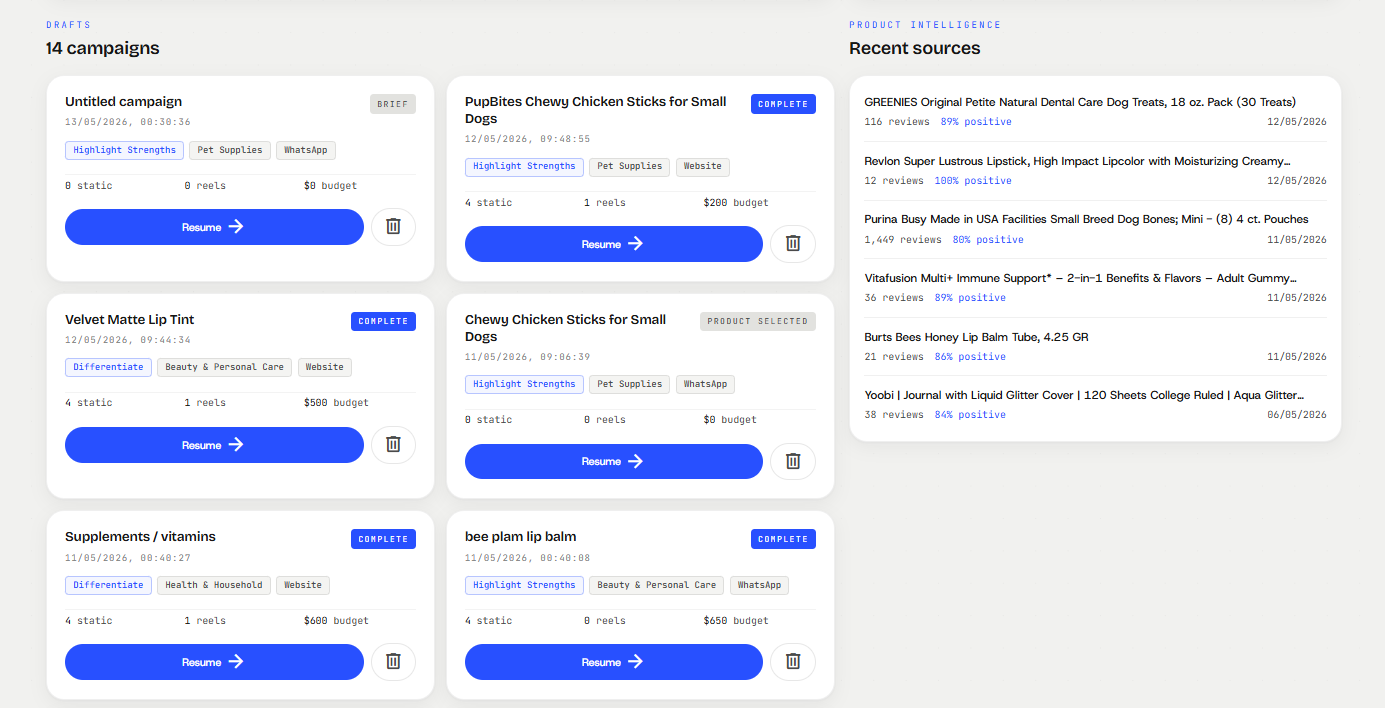
\includegraphics[width=\textwidth]{dash-3}
  \caption{Dashboard, report and product-intelligence history. The user can re-open a completed campaign's report or a previous product-intelligence selection without losing their working state.}
  \label{fig:dash3}
\end{figure}

The dashboard tracks campaigns and reports, not business analytics. It does not pull Shopify revenue, Meta ad performance, or order data; the demonstration runs on a single SQLite file and reports only on the campaigns the user has generated through the application. The point is to make the application useful beyond a one-shot generation flow: returning to a draft is one click, reading a previous report is one click, and a recent product-intelligence selection can be reused on the next campaign without re-walking the brief.

\subsection{Implementation and runtime}
\label{sec:webapp}

\Cref{sec:webjourney} walked the application from the user's side. This subsection documents the same surface as an engineered system. It covers the technology stack, the server-side API, the data layer, the asset and state handling, the runtime path that ties those layers together, and the honest scope of the demonstration.

\subsubsection{Technology stack}
\label{sec:webstack}

The application is a single Next.js project that bundles the user-facing screens and the server-side API into one codebase. The stack is summarised in \cref{tab:webstack}.

\begin{table}[ht!]
  \centering
  \caption{Technology stack of the MarketMind web application.}
  \label{tab:webstack}
  \small
  \begin{tabular}{@{}>{\raggedright\arraybackslash}p{1.8in}>{\raggedright\arraybackslash}p{1.3in}>{\raggedright\arraybackslash}p{2.6in}@{}}
    \toprule
    Layer & Component & Role in MarketMind \\
    \midrule
    Application framework & Next.js 16 (App Router) & Single project for the UI and the API; server routes and client components colocated. \\
    \addlinespace
    UI runtime & React 19 + TypeScript 5 & Typed component tree across every screen; state shared through hooks and route parameters. \\
    \addlinespace
    Styling & Tailwind CSS 4 (PostCSS) & Utility-first styling with brand tokens kept inline so the visual surface matches the design language used in the deck and the report figures. \\
    \addlinespace
    Generation SDK & @google/genai 1.48 & Unified client for Gemini text generation, Nano Banana Pro image generation, and Veo 3.1 Fast video generation. One SDK, three model surfaces. \\
    \addlinespace
    Persistence & SQLite via better-sqlite3 12.9 & Local single-file database holding two tables: \texttt{users} (email + hashed password) and \texttt{drafts} (every campaign in any state, with a status field that walks from brief through stages 1--3 to complete). \\
    \addlinespace
    Email delivery & Resend 6.12 & Transactional email API used by the send-email route to deliver the rendered campaign report to the user's inbox. \\
    \addlinespace
    Report export & html2canvas + jspdf & Client-side rendering of the campaign view into a PDF for download, keeping the on-image text and the paste-into-Meta caption on separate rows. \\
    \bottomrule
  \end{tabular}
\end{table}

\subsubsection{Server-side API surface}
\label{sec:webroutes}

The application's API is a set of typed Next.js server routes, each one focused on one job. \Cref{tab:webroutes} lists every route, the model or service it calls, and the role it plays in a normal session.

\footnotesize
\renewcommand{\arraystretch}{1.05}
\begin{longtable}{@{}>{\ttfamily\raggedright\arraybackslash}p{1.95in}>{\raggedright\arraybackslash}p{1.45in}>{\raggedright\arraybackslash}p{2.15in}@{}}
  \caption{MarketMind server routes. Each route is a single-job endpoint under \texttt{/api/}.}\label{tab:webroutes}\\
  \toprule
  \normalfont Route & \normalfont Service or model & \normalfont Role \\
  \midrule
  \endfirsthead
  \multicolumn{3}{@{}l@{}}{\normalfont\textit{Table \thetable\ continued from previous page}}\\
  \toprule
  \normalfont Route & \normalfont Service or model & \normalfont Role \\
  \midrule
  \endhead
  \midrule
  \multicolumn{3}{r@{}}{\normalfont\textit{Continued on next page}}\\
  \endfoot
  \bottomrule
  \endlastfoot
  /api/auth/login & SQLite users table + session cookie & Local demo login: takes an email and a six-character minimum password, hashes and verifies against the \texttt{users} table, and sets a signed session cookie. New emails are created on first login and seeded with sample drafts. \\
  \addlinespace
  /api/session & Session cookie & Reads the current session and returns the signed-in email, or clears the cookie on sign-out. \\
  \addlinespace
  /api/rank & Local artifact (\texttt{product\_intelligence.json}) & Returns a goal-aware ranked list of similar products under one of the three strategies (highlight strengths, address objections, differentiate). \\
  \addlinespace
  \seqsplit{/api/generate-campaign} & Gemini text & One call per funnel stage; returns the structured creative block JSON (audience, budget split, messaging angle, both copy surfaces, design direction, visual concept). \\
  \addlinespace
  /api/generate-image & Nano Banana Pro & Produces one 4:5 portrait static creative per call, with on-image text rendered by the model and promo badges only when the user supplied price or sale fields. \\
  \addlinespace
  /api/generate-video & Veo 3.1 Fast & Produces one 9:16 visual-only 8-second clip per stage; carries an upstream brand-guideline brief into the video prompt when one is uploaded. \\
  \addlinespace
  /api/generate-logo & Nano Banana Pro & Produces a flat 2D logo under geometry and theme presets on a white background. \\
  \addlinespace
  \seqsplit{/api/generate-concept-image} & Nano Banana Pro & Produces a square concept-product render from a short description; can reuse the generated or uploaded logo on the rendered packaging. \\
  \addlinespace
  \seqsplit{/api/generate-brand-guidelines} & Gemini text + image read & Reads an uploaded product image and returns a self-contained HTML brand guideline with palette, typography, voice, and usage rules. \\
  \addlinespace
  \seqsplit{/api/normalize-themes} & Gemini text & Normalises and dedupes the extracted review themes in small batches before they reach the prompt builder. \\
  \addlinespace
  /api/refine-block & Gemini Flash & Edits one creative block while keeping strategy, audience, interests, and budgets locked. \\
  \addlinespace
  \seqsplit{/api/drafts}, \seqsplit{/api/drafts/[id]} & SQLite drafts table & Lists, creates, reads, patches, and deletes campaign drafts keyed by the signed-in email. A draft carries its brief, selected product, generated stages, and a status field that promotes the same row from brief, through stage~1--3, to complete. \\
  \addlinespace
  /api/send-email & Resend & Sends the rendered campaign report by email; the subject and body lead with the user-facing campaign name. \\
\end{longtable}
\normalsize

Three properties of this API surface are worth naming. The first is that each route is single-job: the campaign generator does not also generate images, the image generator does not also rank products, and the refinement endpoint cannot edit strategy. This matches the contribution claim that each link in the loop can be inspected, tested, and replaced independently. The second is that the routes return typed JSON rather than free-form text, so the client never has to parse model output by regex. The third is that asset uploads (the product image, the brand-guidelines PDF, the user's logo) go through the routes as \texttt{FormData} multipart payloads, which keeps the image bytes out of the JSON body and lets the same route accept structured fields alongside the file.

\subsubsection{Data layer}
\label{sec:webdata}

The persistence layer is a single SQLite database file accessed through the \texttt{better-sqlite3} synchronous binding. Two tables carry the demonstration's state. The \texttt{users} table keys each account on a normalised email and stores a hashed password plus the created-at timestamp. The \texttt{drafts} table holds every campaign the user has ever started, in any state, as a single row that carries the brief, the selected product, the generated stages, and a status field that walks the same row from brief, through stage~1--3, to complete; in-progress and finished campaigns therefore live in the same table, distinguished only by status. The dashboard aggregates (budget total, creative counts by type, funnel mix, recent product-intelligence selections) are computed on read from this table and are not separately stored. The session itself lives in a signed cookie issued by \texttt{/api/auth/login} rather than in a database row. The schema is small by design. The demonstration is a single-user, single-machine system; there is no row-level access control, no migration tooling, and no archival policy beyond what the local file holds.

\subsubsection{State, persistence, and asset handling}
\label{sec:webstate}

The brief is built across six gated steps and is committed as a single draft row only once the user submits at the end of the brief; downstream screens then patch the same row through \texttt{/api/drafts/[id]} as the user picks a product, fills the brand panel, generates each stage, and refines individual blocks. A closed tab or a refreshed browser therefore resumes from the last patched state. The Campaign Output screen runs a small live-normalisation step on the extracted review themes by calling \texttt{/api/normalize-themes} in batches, so the prompt builder sees a clean and de-duplicated theme set without forcing the user to wait on a single long normalisation call. Image and PDF uploads (product image, brand-guidelines PDF, user logo) are sent as \texttt{FormData} multipart payloads; on the server they are read into memory and passed straight into the generation SDK rather than written to a persistent file system, which keeps the demonstration self-contained on a single machine.

\subsubsection{Runtime path}
\label{sec:webruntime}

During a normal run the brief creates the campaign constraints. The \texttt{/api/rank} route reads the offline \texttt{product\_intelligence.json} artifact and returns the goal-aware shortlist. The user's chosen product carries its sentiment profile and curated review excerpts into the \texttt{/api/generate-campaign} route, which makes one call per funnel stage and returns a typed creative-block JSON. Each block then drives a downstream generation call: \texttt{/api/generate-image} for the 4:5 portrait statics, \texttt{/api/generate-video} for the 9:16 hero clip, and \texttt{/api/normalize-themes} for the live theme cleanup that the prompt builder reads on the next iteration. Completed stages are persisted through \texttt{/api/drafts}; the final campaign is rendered into the Campaign Output view and can be exported as a PDF or emailed through \texttt{/api/send-email}. At every step in this path the evidence drawer remains accessible, so the same review excerpts that grounded a creative block at generation time stay readable from the rendered output afterwards.

\subsubsection{Honest scope}
\label{sec:webscope}

The application runs locally on the developer machine for the demonstration. Authentication is a local email and password against a single SQLite file, with a signed session cookie issued at login; there is no production identity layer (no email verification, no password reset, no OAuth, no account management, and no hosted identity provider). Persistence is a single local SQLite file; there is no multi-user load test, no production hosting, and no backup or archival policy beyond the file itself. Real ad-spend testing on Meta is out of scope and is named in \cref{ch:conclusion} as future work, since it requires paid spend and platform credentials that an academic project does not normally have access to. The deliverable proves that the offline pipeline and the generation models can be driven end-to-end by a non-technical user from a single web surface; it does not pretend to be a production marketing platform.


% --------------------------------------------------------------
\chapter{Results and Discussion}
\label{ch:results}
% --------------------------------------------------------------

The classifier and the ranking layer are evaluated quantitatively. The campaign generation step and the production wrapper are evaluated qualitatively. This chapter reports both and then discusses what worked, what did not, and why.

\section{Evaluation methodology}
\label{sec:setup}

The chapter combines five evaluation grades that match what each part of the system can reasonably support. The classifier is evaluated quantitatively on a held-out test set. The ranking layer is evaluated through an algorithmic sanity check on Top-N overlap. The generation step is evaluated through a qualitative side-by-side comparison against a generic prompt across multiple products. The cost figure is an order-of-magnitude viability check against published list prices. The key steps walkthrough demonstrates the deliverable end-to-end. Each grade is reported in its own section, and their combined limits are summarised at the end of the chapter.

The cleaned dataset of 49,989 reviews was split into three sets at the product level using GroupShuffleSplit on the product identifier. The split is approximately 31,000 training reviews, 8,000 validation reviews, and 10,505 test reviews, with zero product overlap across the three sets. Both classifiers are evaluated on the same 10,505-review test set so that any difference comes from the model and not from the data.

The DistilBERT model was trained on a free Colab T4 GPU with the hyperparameters listed in \cref{sec:distilbert}. The validation set was used to pick the best epoch by macro F1; the test set was seen exactly once at the end of training, after the best epoch was already chosen. Random seeds were fixed for NumPy, PyTorch, and CUDA (cudnn.deterministic was set to true), so the run is reproducible.

The ranking sanity check uses the 1,357 products with at least ten reviews. For each product category, the top-N similar products are pulled under each of the three campaign goals, and the Jaccard overlap is computed between the resulting lists. The generation comparison covers four examples in four categories under the same prompt structure: one full campaign-text and image comparison plus three image-only checks (\cref{sec:ablation}). The cost-effectiveness check (\cref{sec:cost}) draws from Google's published Gemini API pricing page and from published GCC agency rate cards, all accessed on 2026-05-10. The key steps walkthrough (\cref{sec:walkthrough}) is qualitative.

\begin{table}[ht!]
  \centering
  \caption{Evaluation map. Each row is reported in its own section.}
  \label{tab:evalmap}
  \small
  \begin{tabular}{@{}>{\raggedright\arraybackslash}p{1.35in}>{\raggedright\arraybackslash}p{1.65in}>{\raggedright\arraybackslash}p{1.55in}>{\raggedright\arraybackslash}p{1.55in}@{}}
    \toprule
    Evaluation target & Evidence used & What it supports & Main limitation \\
    \midrule
    Classifier (\cref{sec:classresults}) & 10,505-review held-out test set, two models, same metrics & Quantitative claim that DistilBERT beats the TF-IDF + LR baseline on the same data & Class imbalance; neutral class is genuinely hard \\
    \addlinespace
    Ranking sanity check (\cref{sec:rankcheck}) & 1,357 products, three goals, Top-N Jaccard overlap & Confirms the goal changes which products surface & Descriptive only, not an optimality claim \\
    \addlinespace
    Generation comparison (\cref{sec:ablation}) & One full campaign example (YumSticks) plus three image-only examples, generic vs structured prompt & Qualitative content advantage of the structured prompt & Single-rater, no paid Meta delivery test \\
    \addlinespace
    Cost-effectiveness check (\cref{sec:cost}) & Google list prices and GCC agency rate cards, accessed 2026-05-10 & Order-of-magnitude viability, not a substitute claim & List prices change; agency package excludes named services \\
    \addlinespace
    Key steps walkthrough (\cref{sec:walkthrough}) & End-to-end user-journey coverage in \cref{sec:webjourney} with screenshots of every screen of the live web application & Demonstrates the deliverable end-to-end & Single-machine demo, no real authentication \\
    \bottomrule
  \end{tabular}
\end{table}

\section{Classifier results}
\label{sec:classresults}

The two classifiers were compared on the same 10,505-review test set. The DistilBERT model beats the baseline on every metric and on every class.

\begin{table}[ht!]
  \centering
  \caption{Headline metrics on the test set.}
  \label{tab:headline}
  \begin{tabular}{@{}lcc@{}}
    \toprule
    Metric & Baseline (TF-IDF + LR) & DistilBERT \\
    \midrule
    Accuracy   & 0.831 & \textbf{0.872} \\
    Macro F1   & 0.611 & \textbf{0.673} (+0.062) \\
    \bottomrule
  \end{tabular}
\end{table}

\begin{table}[ht!]
  \centering
  \caption{Per-class metrics on the test set (precision, recall, F1).}
  \label{tab:perclass}
  \begin{tabular}{@{}llccc@{}}
    \toprule
    Class & Model & Precision & Recall & F1 \\
    \midrule
    Positive & TF-IDF + LR & 0.959 & 0.882 & 0.919 \\
    Positive & DistilBERT  & 0.970 & 0.922 & \textbf{0.945} \\
    \addlinespace
    Negative & TF-IDF + LR & 0.552 & 0.660 & 0.601 \\
    Negative & DistilBERT  & 0.686 & 0.694 & \textbf{0.690} \\
    \addlinespace
    Neutral  & TF-IDF + LR & 0.246 & 0.427 & 0.312 \\
    Neutral  & DistilBERT  & 0.311 & 0.501 & \textbf{0.384} \\
    \bottomrule
  \end{tabular}
\end{table}

The biggest gain is on the negative class (F1 +0.089). The neutral class still has the lowest score on both models, which matches the difficulty of the 3-star reviews described in \cref{sec:dataset}.

The misclassification count drops from 1,775 of 10,505 with the baseline (16.9 percent) to 1,341 of 10,505 with DistilBERT (12.8 percent). The biggest drop is in positive-to-negative confusions (341 down to 145), which suggests that the contextual model handles sarcasm and back-handed compliments better than bag-of-words features can. Confusion matrices for both models are shown in \cref{fig:confusion}.

\begin{figure}[ht!]
  \centering
  \begin{minipage}{0.48\textwidth}
    \centering
    \textbf{TF-IDF + Logistic Regression}\\[6pt]
    \begin{tabular}{@{}lccc@{}}
      \toprule
       & Pred Pos & Pred Neu & Pred Neg \\
      \midrule
      Pos & \textbf{7,800} & 697 & 341 \\
      Neu & 207 & \textbf{274} & 192 \\
      Neg & 123 & 215 & \textbf{656} \\
      \bottomrule
    \end{tabular}
  \end{minipage}
  \hfill
  \begin{minipage}{0.48\textwidth}
    \centering
    \textbf{DistilBERT (fine-tuned)}\\[6pt]
    \begin{tabular}{@{}lccc@{}}
      \toprule
       & Pred Pos & Pred Neu & Pred Neg \\
      \midrule
      Pos & \textbf{8,151} & 545 & 145 \\
      Neu & 176 & \textbf{329} & 171 \\
      Neg & 74 & 230 & \textbf{685} \\
      \bottomrule
    \end{tabular}
  \end{minipage}
  \caption{Confusion matrices on the same test set. Diagonal cells (correct predictions) are in bold. Both models share the same 10,505-review test set. DistilBERT improves every diagonal cell and reduces every off-diagonal positive-row count.}
  \label{fig:confusion}
\end{figure}

\section{Ranking layer sanity check}
\label{sec:rankcheck}

The goal of the ranking layer is not to be optimal; it is to react to the chosen campaign goal. The check therefore measures Top-N Jaccard overlap between the rankings produced under the three goals (highlight strengths, address objections, differentiate) for each product category. Low overlap confirms that the goal really does change which products surface; very high overlap would mean the ranking is not goal-aware in practice.

\begin{table}[ht!]
  \centering
  \caption{Top-10 Jaccard overlap between goal pairs (averaged across categories).}
  \label{tab:jaccard}
  \begin{tabular}{@{}lll@{}}
    \toprule
    Goal pair & Top-10 overlap & Reading \\
    \midrule
    Highlight strengths vs Address objections & Low & Almost different sets \\
    Highlight strengths vs Differentiate      & Moderate & Some overlap \\
    Address objections vs Differentiate       & Low to moderate & Shared volume effects \\
    \bottomrule
  \end{tabular}
\end{table}

The rows above summarise the qualitative pattern observed across the ten product categories. The full per-category overlap matrix is included in the project notebook outputs, which are summarised in \cref{app:percategory}.

\section{Generation comparison: with vs without review evidence}
\label{sec:ablation}

The contribution on the language-model side is the structured prompt. To check whether the structure and the evidence block actually change what the model produces, the same brief is run twice against the same language model with the same decoding configuration. \textbf{Arm~A} sends a short, broad prompt with the basic ad fields requested. \textbf{Arm~B} sends the MarketMind structured prompt with a review-evidence block, caution rules, an output schema, copy rules, and a media rule. The section reports four qualitative examples, not a statistical test. Example~1 (YumSticks, dog treats) is the deep example: it reports both the generated campaign fields and the resulting image, so it carries the full thirteen-row copy table and a generic-vs-MarketMind image comparison. Examples~2 to~4 (Aura, Bambi, TinyGlow) are image-only checks that compare a generic image prompt against the MarketMind image prompt in three further categories; they do not repeat the full campaign-text comparison.

\subsection*{Example 1 --- YumSticks / dog treats (full text and image comparison)}

\subsubsection*{Prompt structures, side by side}

\textbf{Arm~A --- generic prompt.} One short instruction: ``create one Meta ad creative block for dog treats.'' A campaign goal, an audience descriptor, and a tone. A flat list of fields the output should include. No review evidence, no schema, no copy rules, no media rules, no caution rules.

\textbf{Arm~B --- MarketMind prompt.} A campaign-stage context (cold-audience Stage~1). A review-intelligence block with positive evidence and friction or caution evidence. Fourteen numbered output fields covering objective rationale, audience, budget split, messaging angle, two distinct copy surfaces, and design direction plus visual concept. Copy rules (word counts, punctuation, single emoji on the Meta caption). A media rule (4:5 portrait static feed ad).

\subsubsection*{Generated copy, field by field (dog treats / soft chicken-flavor)}

{%
\small
\begin{longtable}{@{}p{1.3in}>{\raggedright\arraybackslash}p{2.2in}>{\raggedright\arraybackslash}p{2.2in}@{}}
  \caption{Example~1, YumSticks: side-by-side copy output.}
  \label{tab:ablation} \\
  \toprule
  Field & Arm A (generic) & Arm B (MarketMind) \\
  \midrule
  \endfirsthead
  \toprule
  Field & Arm A (generic) & Arm B (MarketMind) \\
  \midrule
  \endhead
  \midrule
  \multicolumn{3}{r}{\emph{continued on next page}} \\
  \endfoot
  \bottomrule
  \endlastfoot
  Campaign objective & Sales (Conversions). & Sales (Conversions). \\
  \addlinespace
  Stage 1 rationale & \emph{Not requested.} & Cold audience, but optimising for Sales lets the algorithm serve impressions to users with a track record of buying pet supplies in-feed, so the budget hits high-intent prospects. \\
  \addlinespace
  Audience age range & 25--54. & 25--65+. \\
  \addlinespace
  Suggested interests & Dog treats, Pet parents, Natural pet food, BarkBox, Blue Buffalo. Competitor-brand seeded. & Senior dog, Small dog breeds, Dog food, I Love My Dog, Pet supplies. Audience-led, no competitor brands. \\
  \addlinespace
  Budget & \$50 to \$100 per day per ad set. & Stage budget 70\% of total. Block budget 20\% of stage. \\
  \addlinespace
  Messaging angle & \emph{Not separated.} & ``Soft and Tasty Senior Favorite.'' Targets owners of older or smaller dogs. \\
  \addlinespace
  Headline & ``Fuel Their Wags with Real Chicken!'' & ``Soft chicken treats dogs love'' \\
  \addlinespace
  Primary text & Long, three-paragraph caption-style. Invented brand name (YumSticks). & ``USA-made and incredibly soft. A tasty favorite for any pup.'' \\
  \addlinespace
  CTA & Shop Now. & Shop Treats Now. \\
  \addlinespace
  Meta clickable headline & \emph{Not separated.} & ``Their new favorite chicken treat'' \\
  \addlinespace
  Meta caption & ``High protein. Real chicken. 100\% Tail-Waggin' Good.'' & ``Give your older dog a deliciously soft chicken snack they will completely devour today'' \\
  \addlinespace
  Visual direction & 6--10 second video or dynamic GIF. & 4:5 portrait static feed ad. \\
  \addlinespace
  Visual concept & \emph{Combined into visual direction.} & Split-screen: happy older small dog above, product pouch on sunlit floor below. \\
\end{longtable}
}

Both prompts produced a usable Stage~1 ad and both selected Sales (Conversions) as the campaign objective. The differences sit elsewhere. The MarketMind prompt produced a more controlled Stage~1 rationale, an audience-led interest list rather than a competitor-led one, an explicit budget split as percentages rather than a daily dollar range, separated copy surfaces with a tight on-image headline and a different Meta caption, an evidence-grounded messaging angle, and a clearer separation between visual direction and visual concept. The generic prompt produced a fluent ad, but its primary text drifts into caption length, it invents a brand name (YumSticks), and it folds the visual direction and the visual concept into one block.

\subsubsection*{Visual output}

The same prompt structure carries through to image generation. The generic image prompt receives the generic copy direction; the MarketMind image prompt receives the structured visual concept and brand-input rules. Both arms generate a single 4:5 portrait static for the same dog-treat product. The two outputs are shown in \cref{fig:imgcompare}.

\begin{figure}[ht!]
  \centering
  \begin{minipage}{0.48\textwidth}
    \centering
    \textbf{Arm A --- generic image prompt}\\[4pt]
    
\includegraphics[width=\textwidth]{generic-image.jpg}\\[4pt]
    \small Cartoonish stylisation, flat composition, generic packaging, weaker product readability.
  \end{minipage}
  \hfill
  \begin{minipage}{0.48\textwidth}
    \centering
    \textbf{Arm B --- MarketMind image prompt}\\[4pt]
    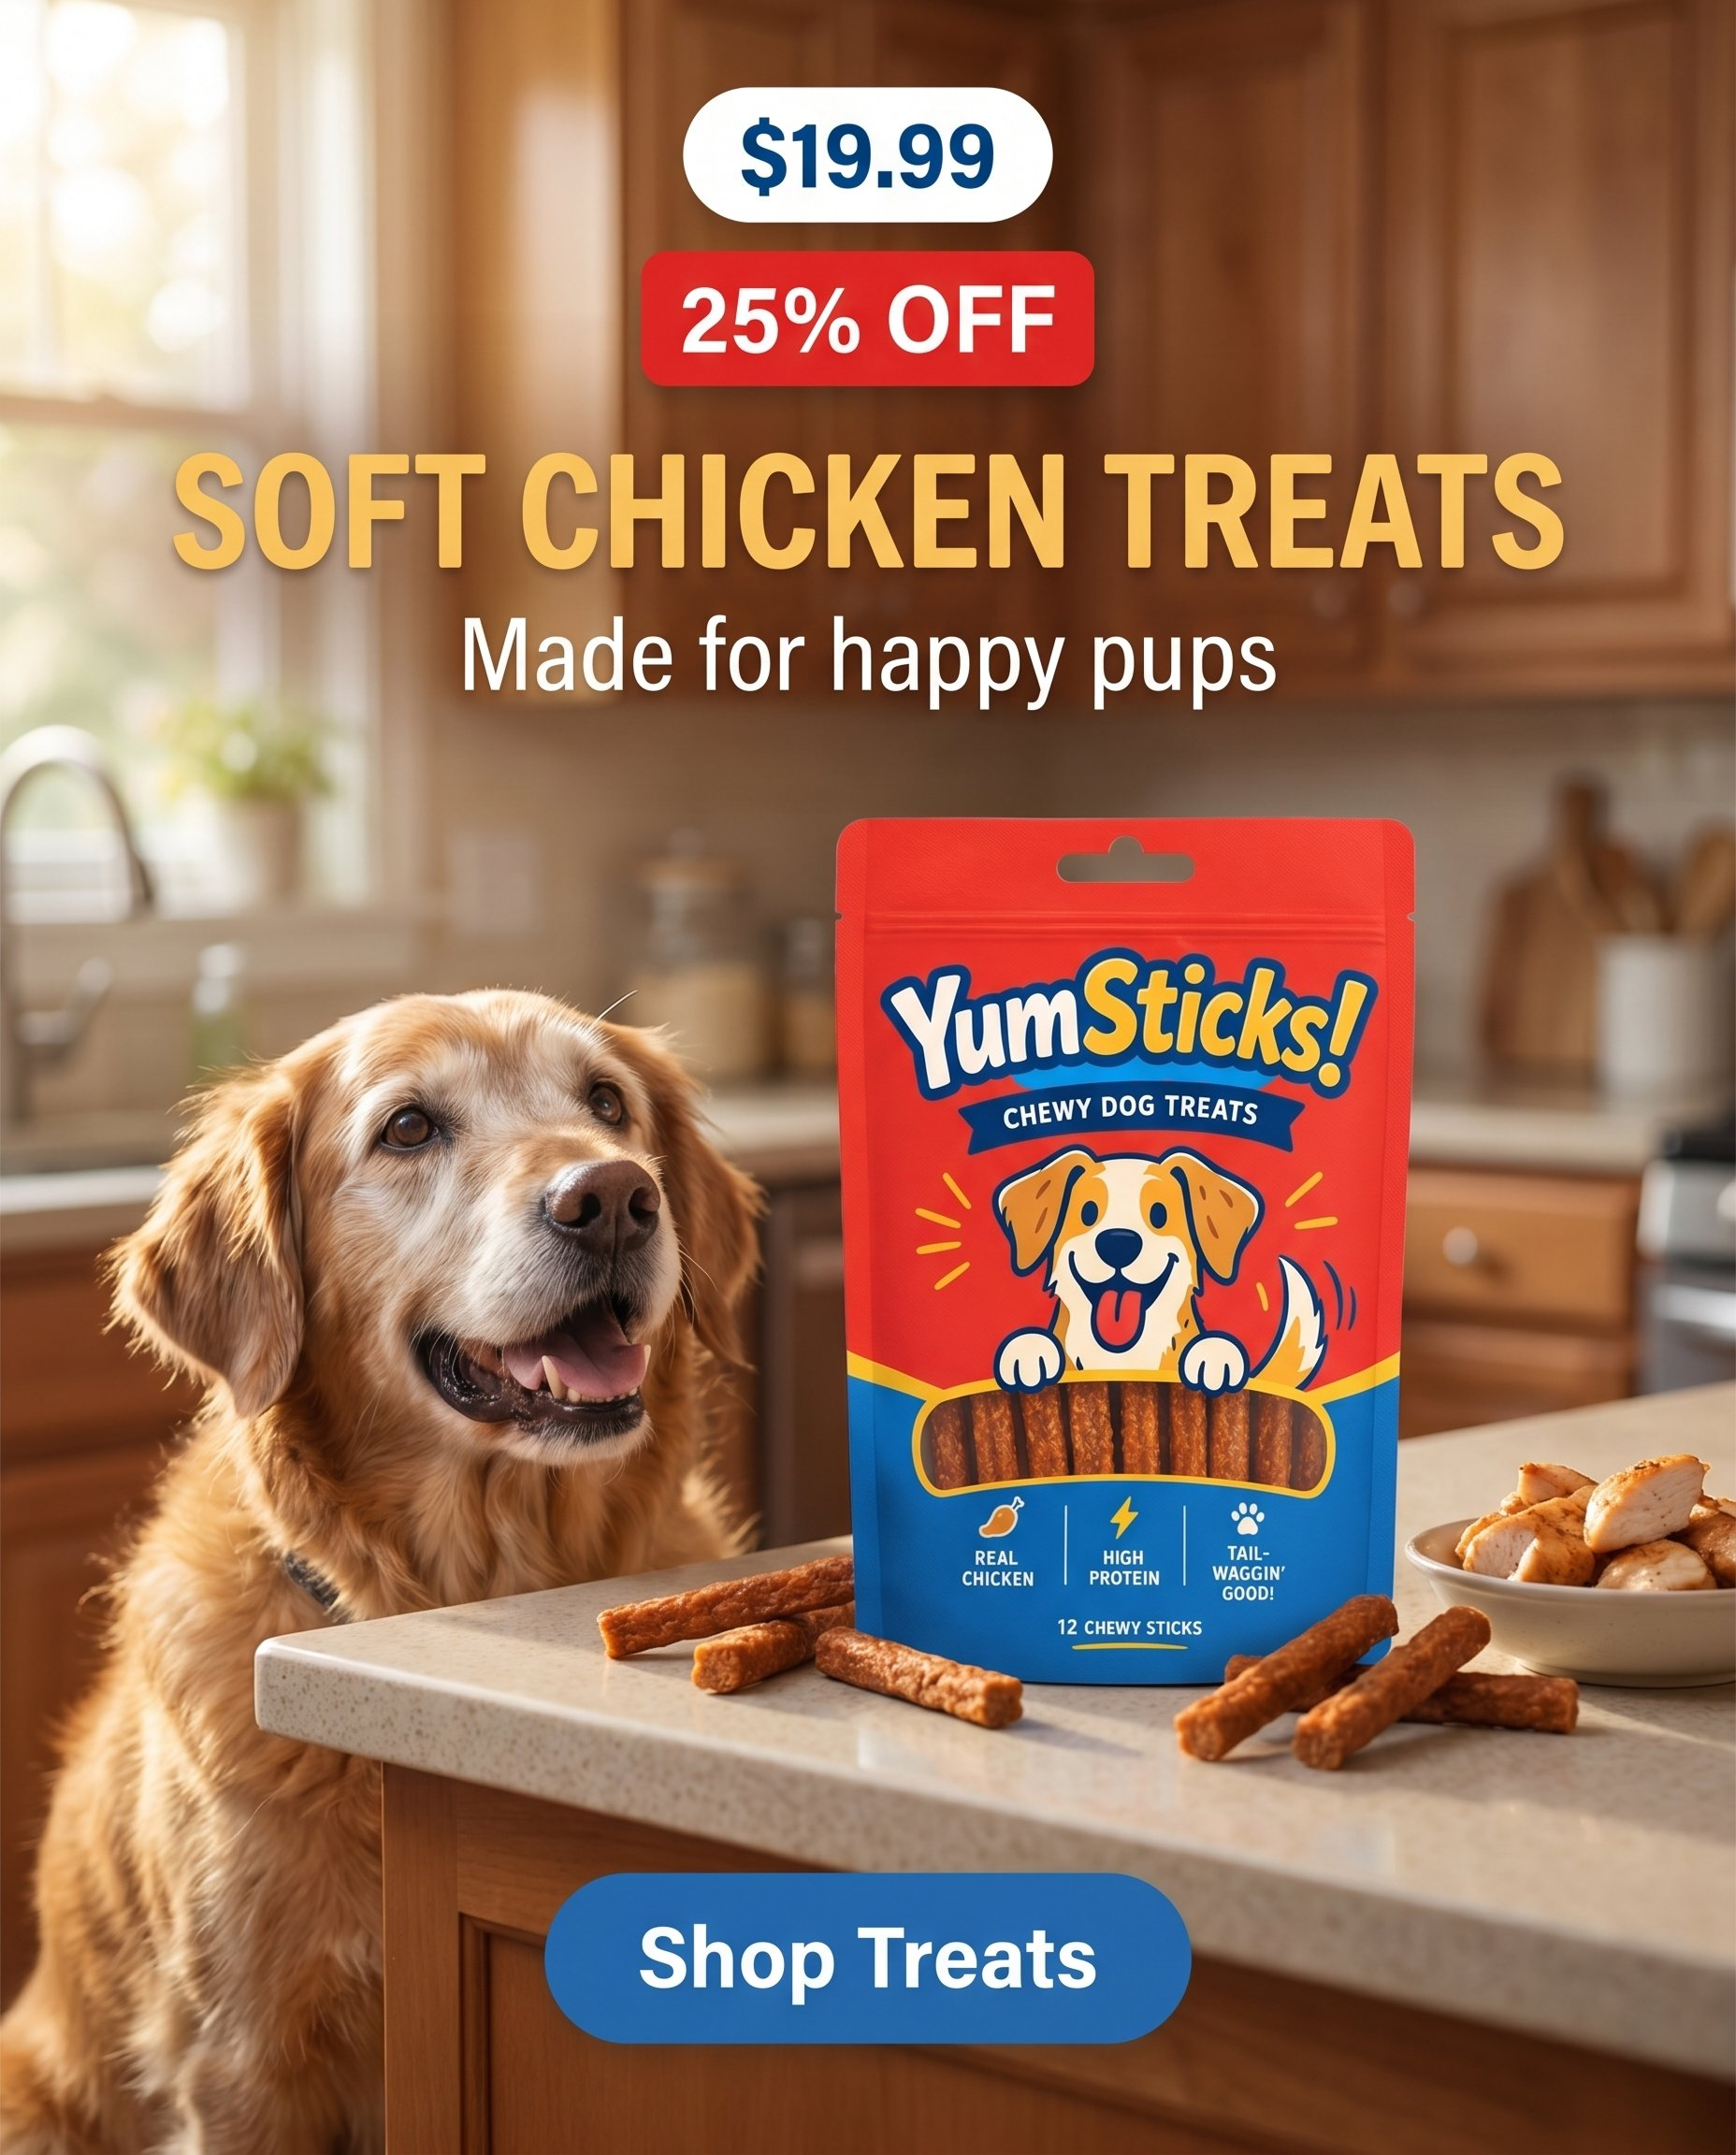
\includegraphics[width=\textwidth]{marketmind-image.jpg}\\[4pt]
    \small Realistic photography, controlled depth of field, clear product showcase, on-image price and discount badge.
  \end{minipage}
  \caption{Example~1, YumSticks: generic image vs MarketMind image (same product, same model).}
  \label{fig:imgcompare}
\end{figure}

The generic image looks more cartoonish and feels cheaper, with weaker product readability and a flatter, more illustrated style. The MarketMind image is closer to a realistic product photograph: warm lighting on the pouch, controlled depth of field that keeps the product in focus, a cleaner composition that matches the structured visual concept (split-screen feel between the dog and the product), and the optional promo signals carried through correctly. The price (\$19.99) and the 25\% OFF badge come from the structured prompt's promo handling, where those fields would be filled in by the user. In the generic prompt, no such fields exist, so the image relies on category visual tropes alone.

\subsubsection*{Summary}

Holding the model and decoding fixed, the structured prompt produced a Stage~1 ad that is more specific to the actual product: the targeting points to senior and small dogs, the messaging angle reuses real review themes (chicken flavor, soft texture, made in the USA), the copy is split across two surfaces with each one obeying its own rules, and the visual is closer to a usable direct-to-consumer pet-brand ad. The generic prompt produced a fluent and similar-looking output, but with broader targeting, an invented brand name, and a more illustrative visual style. On this run the structure plus the review evidence was the difference between a generic-feeling ad and a product-true one.

\textbf{Honest limitations.} One product, one brief, one model run for each arm. The qualitative judgements above are a single-rater read of the generated text and image, not a blind multi-rater study, and the comparison is not statistical. The image differences include a promo badge that exists in the structured prompt's schema but not in the generic prompt; this is part of what the structured prompt contributes, but it also means the two images are not pixel-for-pixel comparable. There is no paid ad-performance test (no Meta delivery, no CTR, no CPA), so this section says nothing about real-world ad results. Arm~B's lift reflects the combined contribution of the review evidence, the structure, the copy rules, the media rule, and the promo handling together, and does not isolate which of those parts contributes how much. The result is an illustrative comparison, not a claim that the structured prompt always produces better copy or better visuals.

\Needspace{4\baselineskip}
\subsection*{Example 2 --- Aura (luxury car diffuser, image-only check)}

Aura is a small luxury car diffuser sold to a premium-leaning audience. This is an image-only check: a generic image prompt (Arm~A) against the MarketMind image prompt (Arm~B), with no campaign-text comparison. The two image outputs are shown in \cref{fig:aura}.

\begin{figure}[ht!]
  \centering
  \begin{minipage}{0.46\textwidth}
    \centering
    \textbf{Arm A --- generic prompt}\\[4pt]
    
\includegraphics[width=\textwidth]{aura-.jpg}
  \end{minipage}
  \hfill
  \begin{minipage}{0.46\textwidth}
    \centering
    \textbf{Arm B --- MarketMind prompt}\\[4pt]
    
\includegraphics[width=\textwidth]{aura-mm.jpg}
  \end{minipage}
  \caption{Example~2, Aura: generic image prompt vs MarketMind image prompt.}
  \label{fig:aura}
\end{figure}

The generic arm leans on competing badges, an ALL-CAPS headline, and decorative emojis on the call-to-action. The structured arm reads as a single value proposition with restrained on-image typography and one clear CTA, which matches Meta's published creative guidance for Feed ads.

\Needspace{4\baselineskip}
\subsection*{Example 3 --- Bambi (premium baby diapers, image-only check)}

Bambi is a premium baby-diaper brand. As with Aura, this is an image-only check: a generic image prompt against the MarketMind image prompt. The two image outputs are shown in \cref{fig:bambi}.

\begin{figure}[ht!]
  \centering
  \begin{minipage}{0.46\textwidth}
    \centering
    \textbf{Arm A --- generic prompt}\\[4pt]
    
\includegraphics[width=\textwidth]{bambi-.jpg}
  \end{minipage}
  \hfill
  \begin{minipage}{0.46\textwidth}
    \centering
    \textbf{Arm B --- MarketMind prompt}\\[4pt]
    
\includegraphics[width=\textwidth]{bambi-mm.jpg}
  \end{minipage}
  \caption{Example~3, Bambi: generic image prompt vs MarketMind image prompt.}
  \label{fig:bambi}
\end{figure}

The generic arm produces multiple competing visual signals (sunburst badges, several value claims at once, a noisy headline) and a small typo in the on-image copy. The structured arm produces a calmer composition with the product anchored visually, a single benefit headline, and a single CTA that matches the category and the audience.

\Needspace{4\baselineskip}
\subsection*{Example 4 --- TinyGlow (sugar-free kids vitamin gummies, image-only check)}

TinyGlow is a sugar-free kids vitamin-gummy brand sold to parents. This is also an image-only check, a generic image prompt against the MarketMind image prompt. The two image outputs are shown in \cref{fig:tinyglow}.

\begin{figure}[ht!]
  \centering
  \begin{minipage}{0.46\textwidth}
    \centering
    \textbf{Arm A --- generic prompt}\\[4pt]
    
\includegraphics[width=\textwidth]{tinyglow-.jpg}
  \end{minipage}
  \hfill
  \begin{minipage}{0.46\textwidth}
    \centering
    \textbf{Arm B --- MarketMind prompt}\\[4pt]
    
\includegraphics[width=\textwidth]{tinyglow-mm.jpg}
  \end{minipage}
  \caption{Example~4, TinyGlow: generic image prompt vs MarketMind image prompt.}
  \label{fig:tinyglow}
\end{figure}

The generic arm reaches for ALL-CAPS shouting, multiple competing claims, and decorative typography that competes with the product. The structured arm puts the product first, leads with the single most relevant parent-facing claim (sugar-free), and uses one restrained CTA.

\subsection*{Across the four examples}

The pattern is consistent across the four examples. The generic arm reaches for visual loudness (badges, shouting type, decorative emojis on the CTA, multiple competing claims) and occasionally trips on small craft errors (typos, invented brand names). The structured arm holds to one headline, one CTA, anchors the product visually, and lets the messaging angle come from a real review theme rather than from category clichés. Only Example~1 carries the full campaign-text comparison; Examples~2 to~4 show the image output alone. None of these comparisons is a statistical test; they are a qualitative panel chosen to illustrate the kind of difference the structured prompt makes when the same brief is processed by the same model.

\section{Cost-effectiveness check}
\label{sec:cost}

The previous section asked whether the structured prompt produces better creative than a generic prompt. A second question matters for the small-seller audience the project targets: whether the cost of running the system on public model APIs sits in a range a one-person store can afford for one or two campaigns per month. This subsection is an order-of-magnitude viability check on published list prices. It is not a like-for-like substitute claim against a marketing agency, and the limits of the comparison are stated explicitly at the end of the subsection.

\subsection*{Per-campaign API cost on Google's published list prices}

A complete MarketMind campaign covers three Meta funnel stages. Each stage runs one structured Gemini text call (Stage 1 cold audience, Stage 2 mid-funnel engagement, Stage 3 sales conversion). Across the three stages the campaign returns roughly eight 4:5 portrait static images and three eight-second 9:16 short videos. Text generation runs on the Gemini 3.1 Pro Preview branch, which is the model the application calls in production, and image and video generation run on Gemini 3 Pro Image Preview (marketed as Nano Banana Pro) and Veo 3.1 Fast respectively. Holding to Google's standard-tier list prices on the Gemini Developer API page~\cite{googlepricing2026}, accessed 2026-05-10, the per-campaign cost decomposes as in \cref{tab:apicost}.

\begin{table}[ht!]
  \centering
  \caption{Per-campaign API cost on Google's standard-tier list prices, accessed 2026-05-10.}
  \label{tab:apicost}
  \small
  \begin{tabular}{@{}>{\raggedright\arraybackslash}p{2.3in}>{\raggedright\arraybackslash}p{2.6in}>{\raggedleft\arraybackslash}p{0.7in}@{}}
    \toprule
    Component & Assumption & Cost (USD) \\
    \midrule
    Text (Gemini 3.1 Pro Preview) & 3 stage calls $\times$ 11k input + 3k output tokens & \$0.17 \\
    \addlinespace
    Static images (Gemini 3 Pro Image Preview, 1K) & 8 images $\times$ \$0.134 per image & \$1.07 \\
    \addlinespace
    Short videos (Veo 3.1 Fast, 1080p) & 3 videos $\times$ 8 seconds $\times$ \$0.12 per second & \$2.88 \\
    \midrule
    \textbf{Per-campaign total} & & \textbf{\$4.13} \\
    \bottomrule
  \end{tabular}
\end{table}

The video line dominates at roughly seventy per cent of the bill. Substituting Veo 3.1 Fast at 720p (\$0.10 per second) drops the video subtotal to \$2.40 and the per-campaign total to about \$3.65. A smaller bundle that produces only ten static ad outputs with on-image copy and a paste-ready caption per output, without the video stage, costs roughly \$1.47 in API spend at the same prices.

\subsection*{Comparison against published GCC agency floors}

The cheapest credibly published monthly retainer found in the GCC for a fixed package that includes graphic design and caption writing for roughly ten to sixteen posts per month is Si3 Digital's Starter tier at \$340 per month (AED 1,249) for nine static posts and three short reels, with the next step at \$680 per month (AED 2,499) for fourteen posts and six reels~\cite{si3packages}. Once paid-ads management is bundled into the same retainer the published floor for a comparable post volume rises to roughly \$2,176 per month (AED 8,000) at Digitalwise~\cite{digitalwisepackages}. As industry guidance rather than a primary rate card, V Patch publishes a basic tier in the \$816 to \$1,360 per month band (AED 3,000--5,000) for twelve to sixteen monthly posts of static graphics, captions, and scheduling on one or two platforms; the same page notes that ad spend is paid directly to the platform and is excluded from these figures~\cite{vpatchpricing}. Currency conversions use the standard AED-to-USD peg of 0.272 throughout.

A Si3 Starter month delivers nine designed static posts plus three short reels. A single MarketMind campaign delivers eight static images plus three short videos, which is in the same creative-volume neighbourhood. \Cref{tab:costcompare} brings the four reference points onto a single USD axis. On those terms a small seller who runs one campaign per month pays around \$340 for the agency-produced version and around \$4 in API fees for the MarketMind-produced version. The comparison is intentionally narrow: it is creative-generation cost only, on published list prices, on a single month's worth of output. The order-of-magnitude reading (roughly two orders of magnitude on this slice) is the only claim being made here, and it sits inside the much narrower question of whether running MarketMind on a public model API is economically feasible for the audience the project targets.

\begin{table}[ht!]
  \centering
  \caption{USD-equivalent cost comparison across the published reference points. AED values shown in parentheses where they help source traceability. The figures are an order-of-magnitude viability check, not a like-for-like substitute claim.}
  \label{tab:costcompare}
  \small
  \begin{tabular}{@{}>{\raggedright\arraybackslash}p{1.55in}>{\raggedright\arraybackslash}p{1.55in}>{\raggedright\arraybackslash}p{0.95in}>{\raggedright\arraybackslash}p{1.55in}@{}}
    \toprule
    Option & Published package or assumption & Approx.\ cost (USD) & What is included or excluded \\
    \midrule
    MarketMind API per campaign & 3 stage text calls + 8 static images at 1K + 3 videos at 1080p, Google list rates~\cite{googlepricing2026} & \$4.13 per campaign & Generation only; human review, strategy, revisions, scheduling, reporting, and media buying are out of scope. \\
    \addlinespace
    Cheapest published content package (Si3 Starter)~\cite{si3packages} & 9 designed posts + 3 short reels per month, one platform & \$340/mo (AED 1,249) & Design, captions, daily monitoring, monthly report; no paid-ads management. \\
    \addlinespace
    Mid-market industry guidance (V Patch Basic)~\cite{vpatchpricing} & 12--16 posts per month, one or two platforms & \$816--\$1,360/mo (AED 3,000--5,000) & Static graphics, captions, scheduling; ad spend excluded; not a primary rate card. \\
    \addlinespace
    Higher tier with ads management (Digitalwise Silver)~\cite{digitalwisepackages} & 10 designed posts per month including ads management & \$2,176/mo (AED 8,000) & Strategy, content management, paid-ads management, monthly analytics. \\
    \bottomrule
  \end{tabular}
\end{table}

\subsection*{What is not in the comparison}

The agency package and the MarketMind output are not interchangeable. The agency price buys account management and client service, ongoing strategy, revision rounds, community management and reply handling, paid-media buying, performance reporting, content scheduling, and brand governance. Language coverage, revision rounds, and account scope can also change package pricing in either direction. None of those line items sit inside the MarketMind output. What the system reduces is the marginal cost of producing a structured, review-grounded campaign draft. It does not replace the rest of what an agency does. Human review, brand judgement, ongoing strategy, and media buying stay outside its scope by design, and the seller still has to make those calls.

The cost numbers above are also list prices on both sides. Google's Gemini prices change, and the prices in \cref{tab:apicost} are the standard-tier figures published on the API pricing page on the access date noted there. Agency retainers shift with scope, region, and seller relationship. The two-orders-of-magnitude figure holds up under a fairly wide multiplier on either side, but the right reading is that the per-campaign cost of running this system on a public model API sits in a different price band from the agency floor for an equivalent volume of designed creative, not that the two produce equivalent business outcomes.

A brief note on latency, since cost and latency travel together for a small seller. The classifier work in this report is a one-time offline preprocessing cost: training and batch inference over the full review corpus run once on a free Colab T4 GPU and produce the per-product profiles that the runtime reads. No per-user-session latency comes from the classifier or the ranking layer at runtime. At runtime the wall-clock cost of a single campaign is dominated by visual generation rather than text: the structured per-stage text call is the fastest part of the pipeline, the static-image calls are slower, and the short-video calls are the slowest. This pattern matches the cost decomposition in \cref{tab:apicost}, where the video line is also the dominant share of the bill. Concrete latency measurements are out of scope for this report.

\section{Key steps walkthrough}
\label{sec:walkthrough}

The end-to-end user journey through the live web application is documented in detail in \cref{sec:webjourney}, with screenshots covering the optional logo and concept-product flows, the brand panel intake, the six-question brief, the product-intelligence display, the campaign generation surface, the evidence drawer, the report preview, and the dashboard. The walkthrough demonstrates that the deliverable runs end-to-end on a single developer machine and that a non-technical user can drive every stage of the pipeline without writing code. The honest scope of the demonstration is recorded in \cref{sec:webscope}.

\section{Discussion}
\label{sec:discussion}

\subsection*{What worked}

The fine-tuned classifier produced a clear lift over the simple baseline on the same test set: accuracy went from 0.831 to 0.872, and macro F1 went from 0.611 to 0.673. The biggest improvement was on the negative class (F1 +0.089), which is where the contextual model handles sarcasm and back-handed compliments better than bag-of-words features. The neutral class also improved (F1 +0.072), although it is still the weakest of the three.

The product-aware split held up. The model never sees the same product across train, validation, and test. The fact that it still generalises tells the right story: it is learning from review language, not from product-specific wording.

The ranking layer reacts to the chosen goal in the way the design intended. Highlight strengths and address objections produce noticeably different rankings, since one favours high-positive products and the other favours mixed-sentiment products. Differentiate produces a third pattern, with some overlap on volume.

On the production side, the structured prompt visibly shapes the output. The on-post text obeys the punctuation rules; the budget percentages sum to 100 in each stage; the brand identity block keeps the user's own product name distinct from the review-source product. The evidence drawer, in particular, makes the grounding visible to the user, which is the part of the system that justifies calling the generation ``grounded'' rather than ``informed.''

\subsection*{What did not}

The neutral class still sits below 0.4 F1. This is a genuine property of the data: 3-star reviews are often a mix of praise and complaints in the same paragraph. A larger labelled corpus and a better backbone would help, but the gap is unlikely to close with the current setup alone.

The image generation step occasionally drops a brand-guideline rule, especially when the guideline is encoded in a complex PDF. The visual output is usable in most cases, but it is not perfect. The short videos are visual-only by design (no audio), which limits how natural they feel. Both are named explicitly as future work.

On the dog-treat product, the ablation in \cref{sec:ablation} made the difference visible. Both arms chose Sales (Conversions). The MarketMind prompt produced a more controlled Stage~1 rationale, an audience-led interest list (Senior dog, Small dog breeds), explicit budget percentages, separated on-image and Meta caption surfaces, an evidence-grounded messaging angle (soft texture, chicken flavor, USA-made trust), and a clearer split between visual direction and visual concept. The generic prompt produced a fluent ad with broader targeting, an invented brand name, and a more illustrative visual style. This is one product, one model, and the limitations are stated under \cref{sec:ablation}.

\subsection*{Significance}

The pattern of ``small trained classifier plus structured prompt plus production wrapper'' is general. It does not only apply to advertising. Any task where a current language model needs to be grounded in a domain-specific signal can adopt the same shape: train a small model on the signal, build a structured profile per item, select representative evidence, and feed both into a fixed prompt schema. The application around it (in this project a web app for small online sellers) decides what users actually do with the output.

\section{Limitations of this evaluation}
\label{sec:evallimits}

The five evaluation grades reported in this chapter do not all carry the same weight, and it is worth saying so directly. The classifier metrics in \cref{sec:classresults} are statistical and reproducible on a fixed test set. The ranking sanity check in \cref{sec:rankcheck} is descriptive: it confirms that the goal changes which products surface, but it is not an optimality claim about the ranking formula itself. The generation comparison in \cref{sec:ablation} covers four examples in different categories, one full campaign-text and image comparison and three image-only checks, all judged by a single rater against criteria taken from Meta's published creative guidance; there is no inter-rater reliability score and no paid Meta delivery test, so the comparison says nothing about real-world ad performance such as click-through or cost per acquisition. The cost figures in \cref{sec:cost} are list-price approximations on both sides of the comparison and will move as Google's API prices and agency rate cards change. The key steps walkthrough in \cref{sec:walkthrough} demonstrates the deliverable end-to-end on a single developer machine and does not test multi-user load, real authentication, or production hosting. Together these grades support the claim that the system works as designed and that the structured prompt produces visibly different creative output; they do not support a stronger claim about marketing performance in the field, and that distinction is preserved throughout the report.


% --------------------------------------------------------------
\chapter{Conclusion and Future Work}
\label{ch:conclusion}
% --------------------------------------------------------------

\section{Conclusion}
\label{sec:conclusion}

This project set out to build a platform that turns real customer reviews into a complete advertising campaign for small online sellers. MarketMind pursues seven high-level goals, listed in \cref{sec:objectives}, and delivers eight system-level contributions, listed in \cref{sec:contributions}.

On the model side, the contributions hold up to inspection. The fine-tuned DistilBERT classifier beats a TF-IDF and Logistic Regression baseline on the same test set across every metric and every class. The classifier is then used to build a per-product sentiment profile for 1,357 products with at least ten reviews. A simple, transparent excerpt-selection step picks the review snippets that the language model will actually see. A goal-aware ranking layer reorders similar products under three campaign goals, and a Jaccard overlap check confirms that the goal really does change the ranking.

On the production side, the structured prompt combines a brand identity block, the chosen review evidence, the user brief, and a fixed output schema. It is called once per funnel stage. The output drives copy on two distinct surfaces, static images, and one short video per stage. The web application turns the pipeline into a usable tool: a six-step brief, a product intelligence screen, a campaign output screen with an evidence drawer, a dashboard, a PDF export, and an email delivery. Drafts auto-save and can be resumed.

The limits of the current system are stated honestly in this report. The neutral class in the classifier is still difficult, since 3-star reviews are genuinely ambiguous. The image generator sometimes drops a brand-guideline rule, and the short videos are visual-only by design. The campaign generation step and the production wrapper are evaluated qualitatively rather than against a paid ad-spend test, since real spend is out of scope for an academic project.

\section{Future work}
\label{sec:future}

The current system has known limits, and the most useful next steps fall into eight directions.

\subsection{Stronger or more recent classifier backbones}

DeBERTa-v3 or a small modern instruction-tuned model could close part of the neutral-class gap with a similar training budget, since the neutral class is the one that most clearly reflects the limits of the current backbone rather than the limits of the data alone.

\subsection{Aspect-based sentiment}

Once a larger and richer review corpus is available, an aspect-level head could attach sentiment to specific product features (battery life, scent, fit, packaging) and feed those directly into the campaign-generation prompt. The current pipeline produces document-level polarity; an aspect head would let the prompt builder pick excerpts by feature rather than by polarity alone.

\subsection{Continual learning on fresh reviews}

A scheduled ingestion step could pull new reviews from the seller's own platform on a regular cadence, with drift detection on the per-product profile and an active-learning queue for low-confidence predictions. This keeps the review intelligence current without retraining the classifier from scratch each time.

\subsection{Real ad-spend testing}

Direct integration with the Meta ad platform would allow a generated campaign to be launched, measured on click-through and conversion, and the results fed back into the ranking layer. This is the single largest missing piece in the current evaluation, since it would convert the qualitative content claims in \cref{sec:ablation} into measured marketing performance.

\subsection{Audio for the short videos}

Voiceover and music synced to the on-post copy, with a silent default and an opt-in toggle, would close the obvious gap between the static images and the short videos in the current output. The default would stay silent to avoid obvious failure modes (mismatched lip sync, incongruent music) until the audio quality is high enough to ship.

\subsection{Multi-language support}

Tokenisation and classifier extension to Arabic, French, and Spanish, with translation-aware evidence selection so the excerpts and the campaign copy share a language. The user-facing flow can stay the same; the offline pipeline learns to handle reviews and produce copy in the buyer's language.

\subsection{Multiple visual backends}

A model-picker per stage that routes to different image and short-video providers, with a small benchmark on cost and quality, would let the system trade resolution against per-call cost on a per-stage basis. The cost-effectiveness check in \cref{sec:cost} already shows that the video line is the dominant per-campaign cost, so a cheaper short-video backend at acceptable quality would change the per-campaign economics directly.

\subsection{Trust signals}

A fake-review filter in front of the classifier, plus a negative-spike anomaly detector that warns the user before they generate a campaign on a product whose reputation is currently dropping. Both are protective of the seller and of the system's grounding claims, since both depend on the input reviews being honest signals.


% --------------------------------------------------------------
% BIBLIOGRAPHY
% --------------------------------------------------------------
\bibliographystyle{IEEEtranN}
\bibliography{references}


% --------------------------------------------------------------
% APPENDICES
% --------------------------------------------------------------
\appendix
% Make TOC entries for appendix chapters read "Appendix A", "Appendix B"...
% by injecting a \renewcommand at this point in the .toc file. Main-body
% chapters processed before this point keep the original (empty) prefix.
\addtocontents{toc}{\protect\renewcommand{\protect\cftchappresnum}{Appendix~}}
\addtocontents{toc}{\protect\addtolength{\protect\cftchapnumwidth}{6em}}

\chapter{Prompt Structure}
\label{app:prompts}

This appendix records the prompt anatomy used by the live web application. It is not a verbatim code dump. The full route files remain the source of record. This format keeps the report readable while still showing how the prompts are structured. The prompt anatomy documented here supports the live application; the qualitative ablation in \cref{sec:ablation} draws on one deep text-and-image example (YumSticks) and three further image-only examples (Aura, Bambi, and TinyGlow).

\section{Gemini 3.1 Pro campaign prompt}
\label{sec:campprompt}

\begin{description}[style=nextline, leftmargin=2cm, labelwidth=1.8cm]
  \item[\textsc{role}] Act as an expert Meta advertising strategist and creative director. Generate one stage of a three-stage funnel, not the whole campaign at once.
  \item[\textsc{user identity}] List user brand name, user product name, and review-intelligence source product separately. Rule: the source product is evidence only and must not become the user's brand or product name.
  \item[\textsc{product context}] Pass category, total reviews analyzed, and sentiment percentages. This tells the model how much evidence is behind the campaign.
  \item[\textsc{campaign brief}] Pass goal, audience, tone chips, business model, and goal-specific guidance. The business model changes CTA language: website, WhatsApp, and app campaigns use different action verbs.
  \item[\textsc{brand availability}] State what is available and what is missing: product image, brand-guidelines PDF, logo image, and free-text notes. Missing assets are named so the model does not invent product packaging or a brand system.
  \item[\textsc{promo rule}] If price or sale percentage exists, static-image concepts may include separate badges. If both are blank, the model is told not to invent prices, discount stickers, or sale claims.
  \item[\textsc{review intelligence}] Supply strengths, complaints, friction points, and direct positive, negative, and neutral excerpts. The model must ground messaging angles in these themes and excerpts.
  \item[\textsc{copy contract}] Separate on-image copy from Meta caption copy. On-image copy is short and punctuation-light. Meta copy is 10--15 words, includes one emoji, and has a business-model-aware soft CTA.
  \item[\textsc{media contract}] Block~1 is a 9:16 visual-only Reel: no text overlays, no CTA button inside the video. Blocks 2 and later are 4:5 portrait static ads with text rendered onto the image.
  \item[\textsc{json schema}] Return only a JSON array. Required fields include objective, stage rationale, audience, interests, stage and block budgets, messaging angle, both copy surfaces, design direction, visual concept, motion direction, and description.
\end{description}

\section{Nano Banana Pro static-image prompt}
\label{sec:imgprompt}

\begin{description}[style=nextline, leftmargin=2cm, labelwidth=1.8cm]
  \item[\textsc{task}] Generate a finished Meta portrait feed-ad image, 4:5 aspect ratio, with headline, primary text, and CTA rendered onto the image.
  \item[\textsc{identity}] Use the user's brand and product. Do not print the review-intelligence source name on the ad.
  \item[\textsc{attachment order}] Document the inline attachments in order: product image first, brand-guidelines PDF second, brand logo third. This helps the model map each reference to the correct role.
  \item[\textsc{reference priority}] Product image wins for product appearance. Brand-guidelines PDF wins for palette and typography. Logo image wins for the brand mark unless the PDF has a clearer official logo.
  \item[\textsc{product fidelity}] If a product image exists, preserve shape, packaging type, proportions, major colors, label placement, and visible cues. Restaging is allowed; replacing the product is not.
  \item[\textsc{brand fidelity}] If a logo exists, place it visibly and do not crop, recolor, distort, or redesign it. If details are hard to reproduce, preserve the closest shape and color relationships.
  \item[\textsc{promo badges}] Render only supplied price or sale badges. Empty promo fields mean no fake prices and no discount claims.
  \item[\textsc{checklist}] Final checklist: same product type, same silhouette, same color cues, supplied logo used, no invented brand, promo badges only when supplied, 4:5 portrait output.
\end{description}

\section{Logo-generation prompt}
\label{sec:logoprompt}

\begin{description}[style=nextline, leftmargin=2cm, labelwidth=1.8cm]
  \item[\textsc{task}] Generate one flat 2D vector-style logo on a clean white background. It is a logo file, not packaging, a mockup, or an ad scene.
  \item[\textsc{inputs}] Use brand name, palette text, optional visual element, geometry preset, and theme preset. The user can ask for wordmark-only by saying no symbol.
  \item[\textsc{geometry}] Choose from simple presets: wordmark, circle badge, angular geometric mark, or rounded icon. This keeps the output bounded and repeatable.
  \item[\textsc{theme}] Choose from modern, outdoor, luxury, playful, rustic, or tech. The theme affects typography, spacing, and color mood.
  \item[\textsc{constraints}] Square 1:1 composition, centered mark, 1--3 colors, legible brand name, no shadows, no 3D, no product photography, no multi-variant grid, no watermarks.
\end{description}

\section{Concept-product prompt}
\label{sec:conceptprompt}

\begin{description}[style=nextline, leftmargin=2cm, labelwidth=1.8cm]
  \item[\textsc{task}] Generate a polished square product concept image from a short user description. The framing is honest: this is a concept render, not production packaging artwork.
  \item[\textsc{composition}] Force a square 1:1 hero shot with the product centered, balanced safe margins, clean lighting, and minimal clutter.
  \item[\textsc{branding}] Create a believable simple brand identity from the product idea, with limited label text and no crowded design.
  \item[\textsc{logo attachment}] When the user supplies a logo, reuse it as the canonical mark on the product surface or as a small corner mark. Do not invent a different logo.
  \item[\textsc{refinement}] When refining, attach the previous concept and change only what the user's instruction asks for. Preserve the core product, packaging category, and brand direction.
\end{description}

\section{Brand-guideline and refinement prompts}
\label{sec:refineprompt}

\begin{description}[style=nextline, leftmargin=2cm, labelwidth=1.8cm]
  \item[\textsc{brand guideline}] Gemini 3.1 Pro reads the product image and returns one self-contained HTML brand guideline. It must include color palette, typography roles, voice, product showcase, and usage rules. The generated HTML is preview and download material; uploaded PDF guidelines remain the direct generation reference.
  \item[\textsc{per-card refinement}] Gemini Flash edits one creative block. Strategy, messaging angle, audience, interests, and budgets are locked. Editable fields are the two copy surfaces, design direction, visual concept, description, and motion direction for Reel blocks.
  \item[\textsc{video support}] For Reels, the route first summarizes an uploaded brand-guidelines PDF into a compact brief, then passes that brief into the Veo prompt for mood, palette, lighting, and photographic feel. The video prompt stays visual-only and forbids added text overlays.
\end{description}

The qualitative ablation evidence for the structured prompt versus a generic prompt lives in \cref{sec:ablation}. This appendix documents prompt structure only. The structured-prompt advantage on the YumSticks example, with limitations, is reported in that section.


\chapter{Sample Campaign Outputs}
\label{app:sample}

The dog-treat run from the \cref{sec:ablation} ablation is the canonical sample campaign for this report. The MarketMind Stage~1 creative block (campaign objective, audience, budget split, messaging angle, on-image headline and primary text, CTA, Meta clickable headline, Meta caption, design direction, and visual concept) is reproduced in \cref{sec:ablation} \cref{tab:ablation}. The two image outputs (generic prompt and MarketMind prompt) are reproduced as \cref{fig:imgcompare} in the same section. No additional sample campaigns are inserted here; the report uses the \cref{sec:ablation} outputs as the representative end-to-end example.


\chapter{Per-Category Classifier Metrics}
\label{app:percategory}

This appendix reports the per-category breakdown of the two classifiers on the same 10,505-review held-out test set described in \cref{sec:setup}. Each row is one of the ten Amazon product categories. \Cref{tab:percatbaseline} reports the TF-IDF and Logistic Regression baseline. \Cref{tab:percatdistil} reports the fine-tuned DistilBERT model, including the neutral-class F1 column because the neutral class is the weakest on every backbone and the most informative for honest assessment.

\begin{table}[ht!]
  \centering
  \caption{Per-category metrics: TF-IDF + Logistic Regression baseline on the 10,505-review test set. Categories sorted alphabetically to match \cref{tab:percatdistil}.}
  \label{tab:percatbaseline}
  \small
  \renewcommand{\arraystretch}{1.05}
  \begin{tabular}{@{}>{\raggedright\arraybackslash}p{2.4in}rrr@{}}
    \toprule
    Category & Count & Accuracy & Macro F1 \\
    \midrule
    Baby Products & 1{,}370 & 0.818 & 0.635 \\
    Beauty and Personal Care & 911 & 0.785 & 0.589 \\
    Electronics & 832 & 0.797 & 0.590 \\
    Health and Household & 886 & 0.805 & 0.595 \\
    Home and Kitchen & 988 & 0.846 & 0.607 \\
    Office Products & 300 & 0.823 & 0.605 \\
    Pet Supplies & 1{,}986 & 0.864 & 0.615 \\
    Sports and Outdoors & 1{,}073 & 0.804 & 0.599 \\
    Tools and Home Improvement & 1{,}104 & 0.843 & 0.616 \\
    Toys and Games & 1{,}055 & 0.878 & 0.613 \\
    \midrule
    \textbf{Overall} & \textbf{10{,}505} & \textbf{0.831} & \textbf{0.611} \\
    \bottomrule
  \end{tabular}
\end{table}

\begin{table}[ht!]
  \centering
  \caption{Per-category metrics: fine-tuned DistilBERT on the same 10,505-review test set. Categories sorted alphabetically. Neutral F1 reported separately because the 3-star class is the hardest class and the one that most clearly reflects backbone limits.}
  \label{tab:percatdistil}
  \small
  \renewcommand{\arraystretch}{1.05}
  \begin{tabular}{@{}>{\raggedright\arraybackslash}p{2.4in}rrrr@{}}
    \toprule
    Category & Count & Accuracy & Macro F1 & Neutral F1 \\
    \midrule
    Baby Products & 1{,}370 & 0.861 & 0.674 & 0.449 \\
    Beauty and Personal Care & 911 & 0.862 & 0.675 & 0.368 \\
    Electronics & 832 & 0.833 & 0.636 & 0.299 \\
    Health and Household & 886 & 0.877 & 0.695 & 0.424 \\
    Home and Kitchen & 988 & 0.879 & 0.647 & 0.340 \\
    Office Products & 300 & 0.877 & 0.697 & 0.467 \\
    Pet Supplies & 1{,}986 & 0.876 & 0.662 & 0.341 \\
    Sports and Outdoors & 1{,}073 & 0.859 & 0.685 & 0.416 \\
    Tools and Home Improvement & 1{,}104 & 0.895 & 0.698 & 0.382 \\
    Toys and Games & 1{,}055 & 0.900 & 0.658 & 0.378 \\
    \midrule
    \textbf{Overall} & \textbf{10{,}505} & \textbf{0.872} & \textbf{0.673} & \textbf{0.384} \\
    \bottomrule
  \end{tabular}
\end{table}

Two observations close this appendix. The first is that DistilBERT beats the baseline on every single category on both accuracy and macro F1: the smallest improvement is on Electronics ($+$0.036 accuracy, $+$0.046 macro F1) and the largest is on Beauty and Personal Care ($+$0.077 accuracy, $+$0.086 macro F1). The second is that neutral F1 is the weakest column across every category, ranging from 0.299 (Electronics) to 0.467 (Office Products); this matches the noise property of 3-star reviews discussed in \cref{sec:dataset}, where the same review can carry praise and complaint in the same paragraph, and explains why the neutral class is the most reliable indicator of where a stronger backbone would still help.


\chapter{Additional Web App Screenshots}
\label{app:screenshots}

This appendix collects additional screenshots of the live web application that did not make it into the main body. They cover four things the body does not show in detail: brief steps in mid-flow, the in-app pipeline transparency panel that summarises every model run that contributed to a campaign, the auto-generated brand-guidelines HTML produced from a product image, and the multi-page exported campaign report.

\section{Brief screen, mid-flow}

\Cref{fig:appbrief3} and \cref{fig:appbrief4} show the Brief screen as the user is mid-way through the six gated questions. The first answers are committed at the top of the page as compact review rows; the active question is open below. The same row pattern carries through the rest of the brief.

\begin{figure}[ht!]
  \centering
  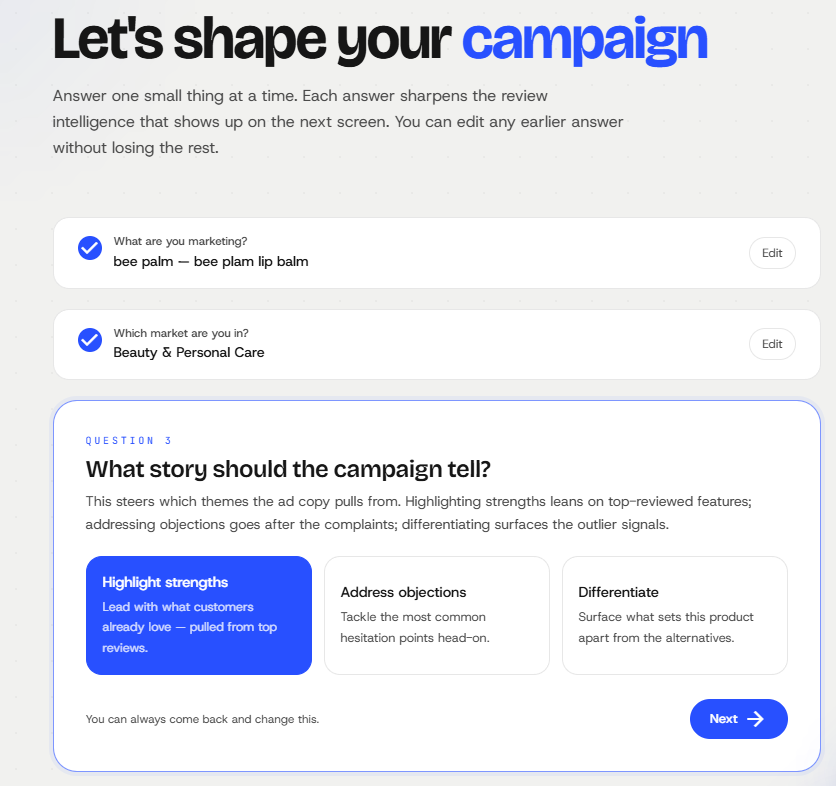
\includegraphics[width=0.7\textwidth]{additional-webapp-2}
  \caption{Brief screen on the active third question (campaign goal). The first two answers are committed and visible as collapsed review rows above; the active card shows the three goal options (highlight strengths, address objections, differentiate) and a Next button gated until the user picks one.}
  \label{fig:appbrief3}
\end{figure}

\begin{figure}[ht!]
  \centering
  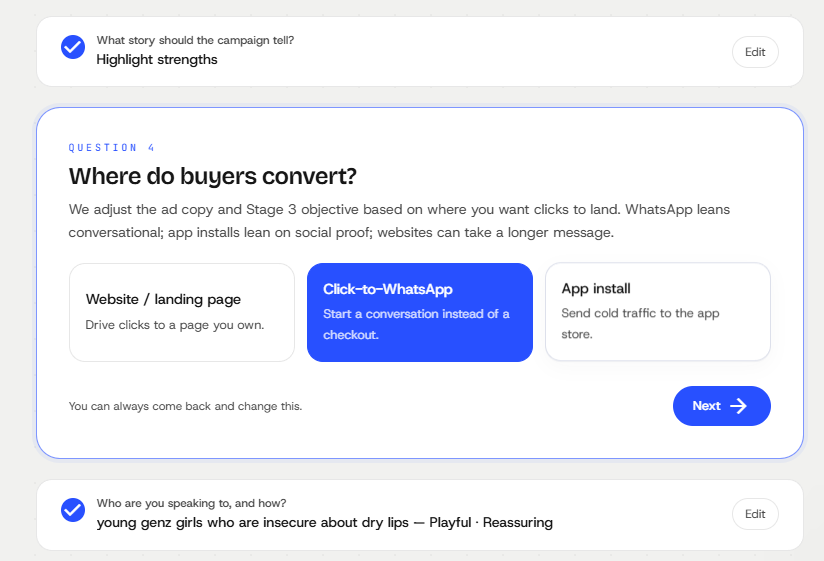
\includegraphics[width=0.7\textwidth]{additional-webapp-3}
  \caption{Brief screen on the active fourth question (business model). The previous answers stay visible at the top so the user can edit any one without losing the rest. Question 4 picks the conversion surface, which downstream changes the call-to-action verbs in the generated copy.}
  \label{fig:appbrief4}
\end{figure}

\section{Pipeline transparency panel}

The Campaign Output screen carries a collapsible \emph{How This Campaign Was Generated} panel that lists every model run behind the campaign with the actual values it produced. \Cref{fig:apppipeline} shows the panel for a PupBites Stage~1 generation. Six steps are named with their concrete outputs: the DistilBERT classifier with the test-set headline metrics ($87.2\,\%$ accuracy, $0.673$ macro F1), the algorithmic product ranking with the source product picked, TF-IDF theme extraction with the strength and complaint counts, Gemini Flash theme normalisation, Gemini 3.1 Pro campaign generation with the per-stage block count, and the Nano Banana Pro + Veo media generation.

\begin{figure}[ht!]
  \centering
  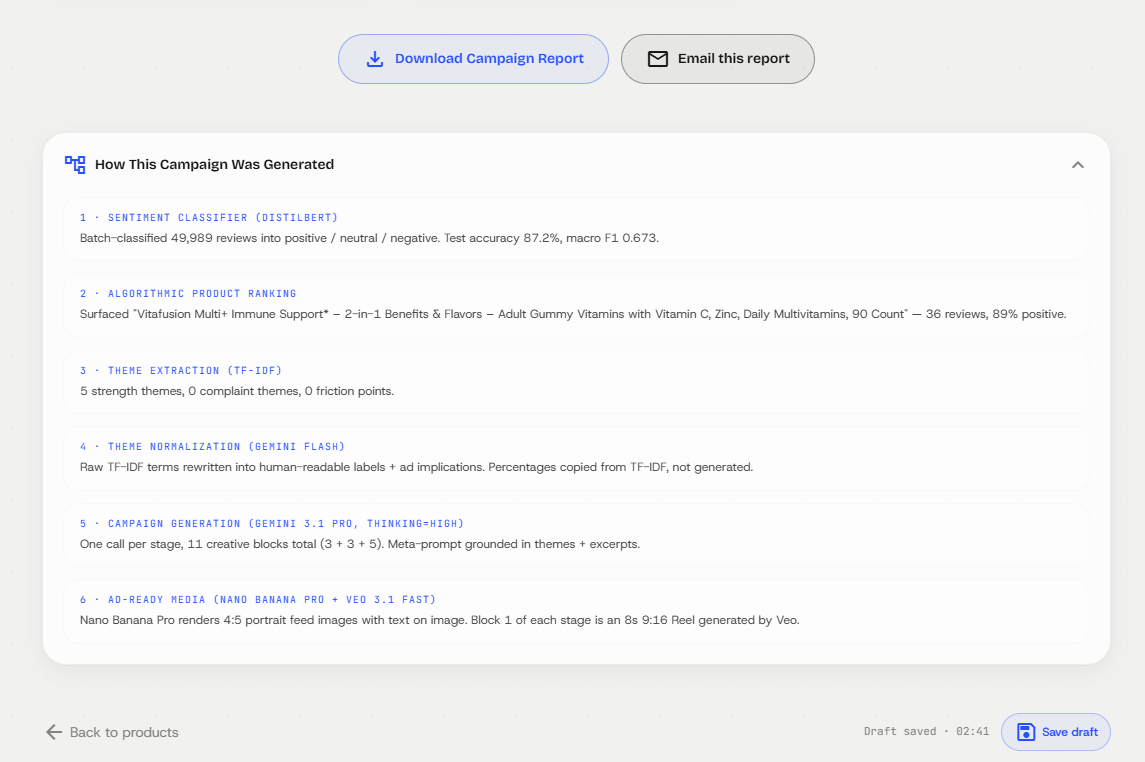
\includegraphics[width=0.7\textwidth]{additional-webapp-1}
  \caption{Pipeline transparency panel on the Campaign Output screen. Six model runs that produced the campaign are named individually with the values they produced. The panel sits above the creative blocks and gives the user a verifiable trace from the offline pipeline to the rendered output.}
  \label{fig:apppipeline}
\end{figure}

\section{Auto-generated brand guidelines}

The brand panel exposes a \emph{Generate from product image} action that calls \texttt{/api/generate-brand-guidelines}, which reads the uploaded product image and returns a self-contained HTML brand guideline. The guideline names a palette with hex codes and usage roles, a typography system with a headline, body, and CTA pairing, do-and-don't rules for photography and ad copy, and a one-line voice statement. The HTML is preview material; once accepted, MarketMind uses the guideline as a structured brand-context input to the downstream image and video prompts, which keeps the rendered creatives more consistent with the brand's palette, typography, voice, and logo than a free-text brand context can on its own. \Cref{fig:appbrandguide1} to \cref{fig:appbrandguide4} show four pages from two generated guidelines: chargeUP! (an energy-charger product) and TinyGlow (kids' vitamin gummies).

\begin{figure}[ht!]
  \centering
  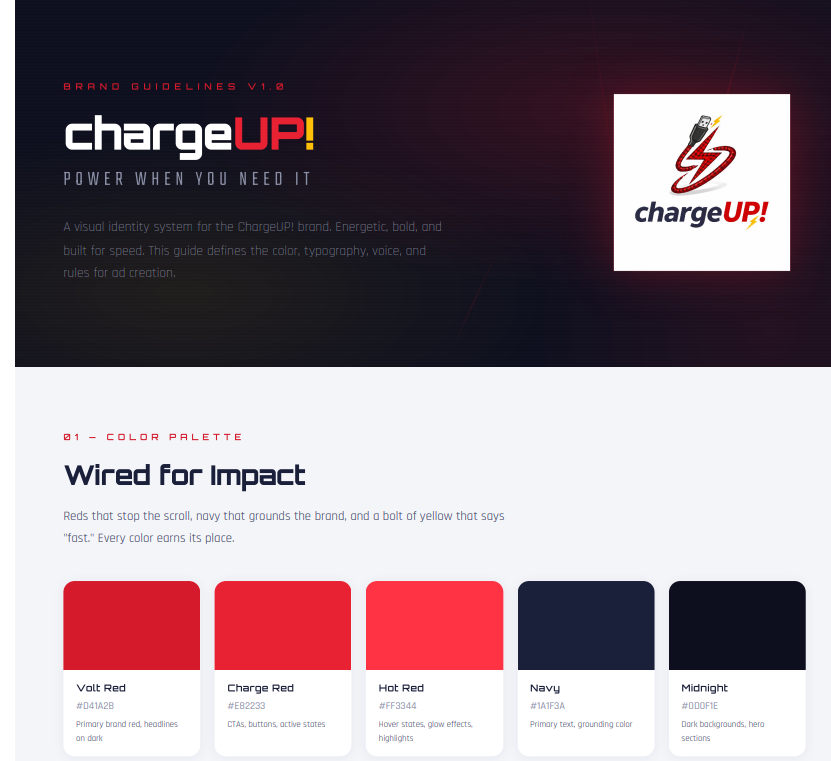
\includegraphics[width=0.7\textwidth]{brand-guide-1}
  \caption{Auto-generated brand guideline for the chargeUP! product, cover and palette page. The palette names five colours with hex codes and usage roles; the right-hand panel shows the logo as anchored on the guideline cover.}
  \label{fig:appbrandguide1}
\end{figure}

\begin{figure}[ht!]
  \centering
  
\includegraphics[width=0.7\textwidth]{brand-guide-2}
  \caption{Auto-generated brand guideline for TinyGlow (kids' vitamin gummies), cover and palette page. The palette is warmer and softer than chargeUP!'s, drawn from the product photo's own colour cues.}
  \label{fig:appbrandguide2}
\end{figure}

\begin{figure}[ht!]
  \centering
  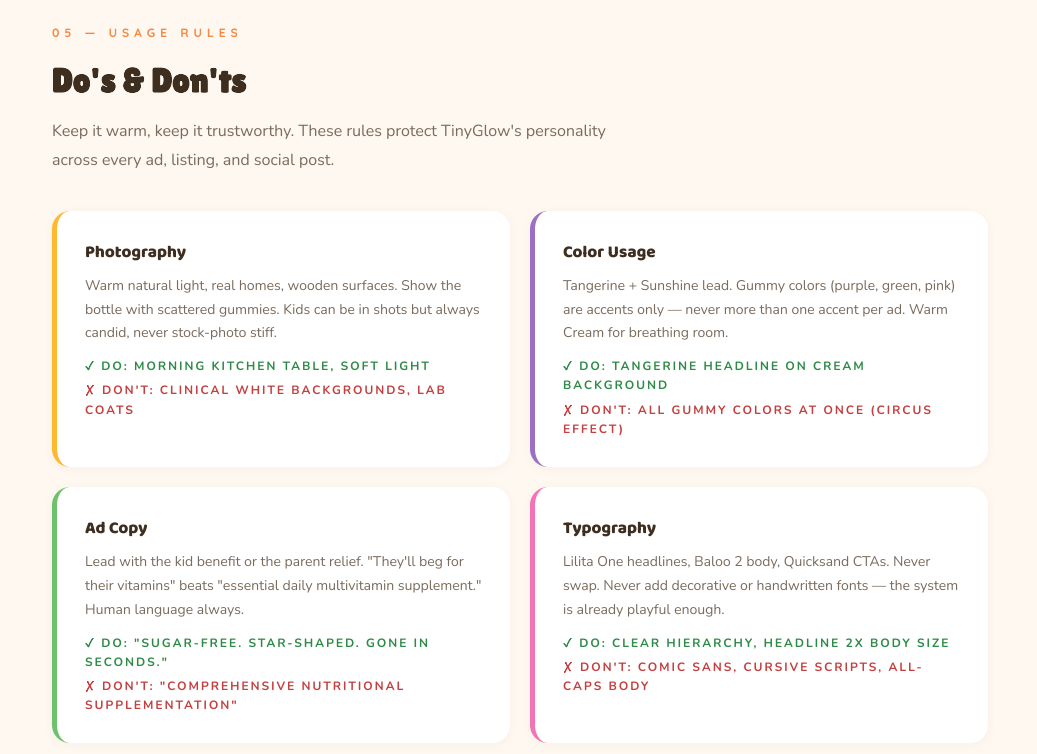
\includegraphics[width=0.7\textwidth]{brand-guide-3}
  \caption{TinyGlow guideline, Do's and Don'ts page. Four panels (photography, color usage, ad copy, typography) give the downstream image-prompt builder concrete usage rules to follow when assembling the visual prompt.}
  \label{fig:appbrandguide3}
\end{figure}

\begin{figure}[ht!]
  \centering
  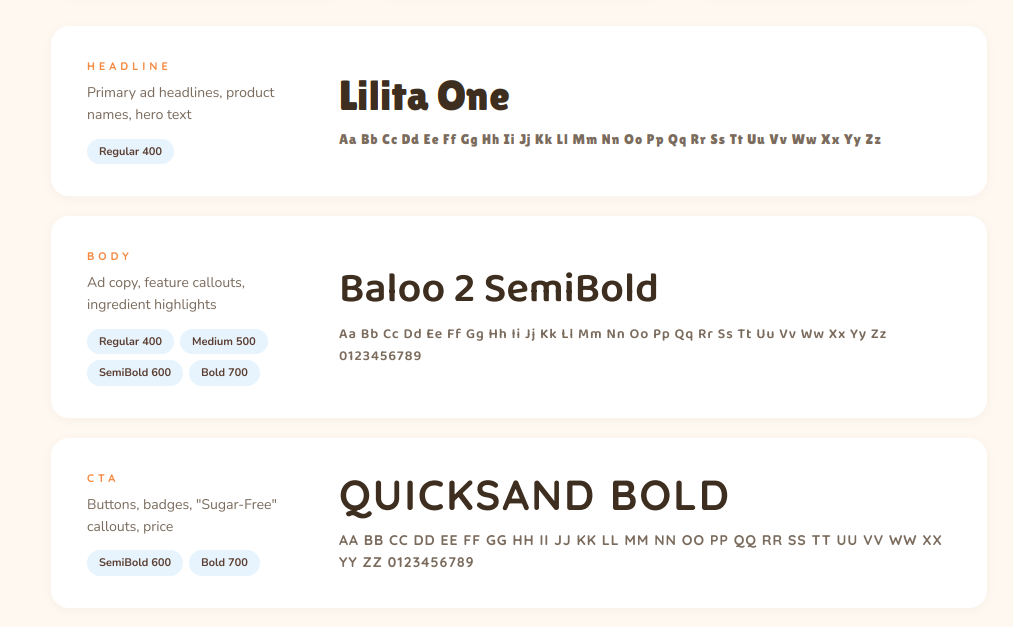
\includegraphics[width=0.7\textwidth]{brand-guide-4}
  \caption{TinyGlow guideline, typography page. The three roles (headline, body, CTA) carry specific fonts and weights; the image prompt builder reads these and the image model renders on-image text at the closest available weight.}
  \label{fig:appbrandguide4}
\end{figure}

\section{Exported campaign report (PDF pages)}

The exported PDF is the deliverable a small seller actually hands to a partner or keeps for their own records. \Cref{fig:appreport1} to \cref{fig:appreport3} show three pages of the PupBites Chewy Chicken Sticks campaign report. Each Stage page carries the full creative block layout (on-post copy and Meta caption on separate rows) so the user can drop the text directly into the Meta ad composer without manual splitting.

\begin{figure}[ht!]
  \centering
  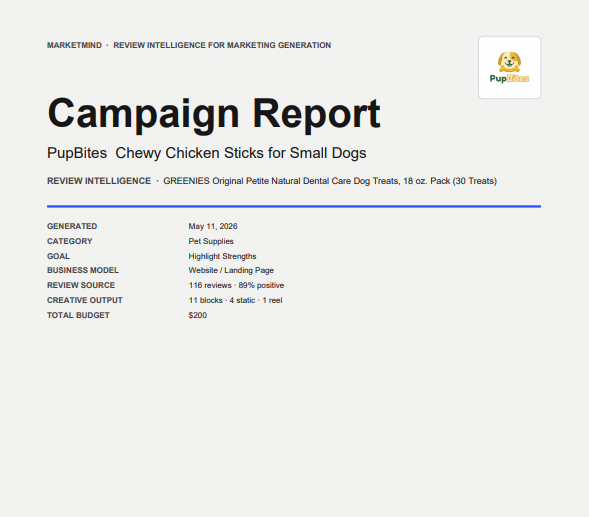
\includegraphics[width=0.7\textwidth]{report-1}
  \caption{Exported PDF, cover page. The user-facing campaign name (PupBites Chewy Chicken Sticks for Small Dogs) leads the page; the review-intelligence source (a real Amazon dog-treat product) sits as the secondary subheader. The cover summarises the brief and the generation stack as a compact block.}
  \label{fig:appreport1}
\end{figure}

\begin{figure}[ht!]
  \centering
  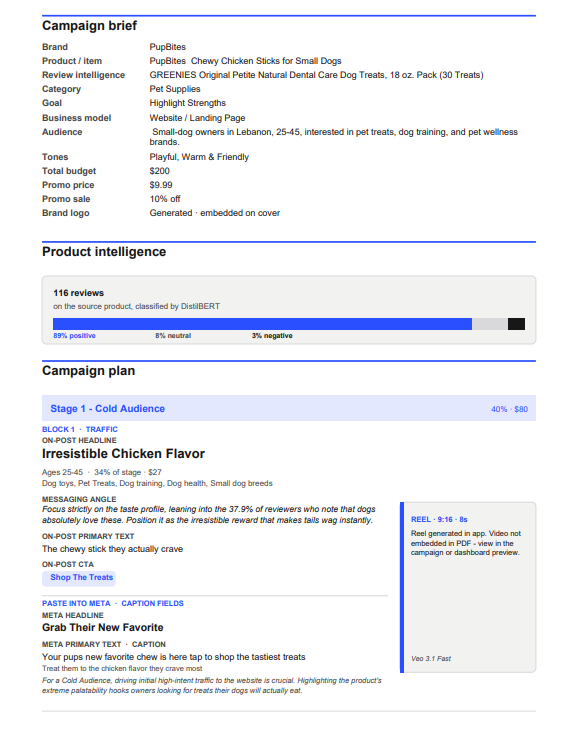
\includegraphics[width=0.55\textwidth]{report-2}
  \caption{Exported PDF, brief and Stage~1 block. The brief is reproduced for traceability, the product-intelligence summary shows the per-class sentiment split, and the Stage~1 creative block lays out the on-post copy, Meta caption, design direction, and reel placeholder side by side.}
  \label{fig:appreport2}
\end{figure}

\begin{figure}[ht!]
  \centering
  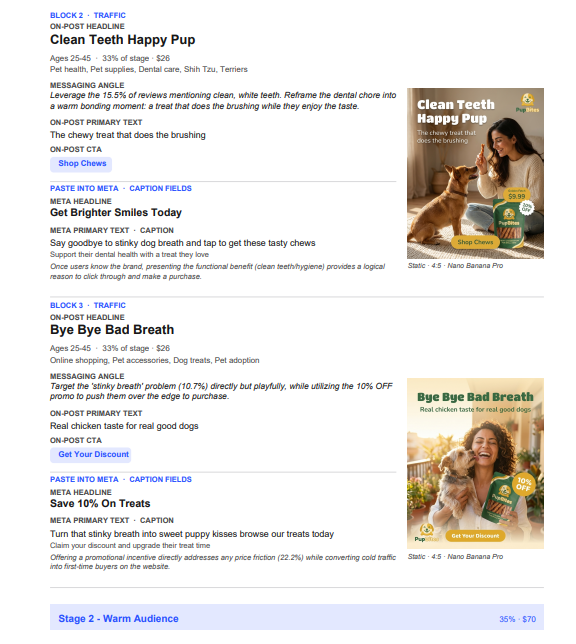
\includegraphics[width=0.55\textwidth]{report-3}
  \caption{Exported PDF, Stage~1 follow-up blocks and start of Stage~2. The static-image creatives sit alongside their copy. The header band at the bottom marks the funnel transition from Stage~1 cold audience to Stage~2 warm-audience retargeting.}
  \label{fig:appreport3}
\end{figure}


\chapter{Sample Logos and Creative Assets}
\label{app:logos}

A short gallery of representative outputs from the in-app generators and the campaign generation pipeline. The aim is to give the reader a feel for the visual surface that the production wrapper produces, not to argue that any single output is best. All assets are rendered by the application; none of them are designed by hand.

\section{Logos}

\Cref{fig:applogos1} to \cref{fig:applogos3} show three logos rendered by the in-app logo generator under different geometry and theme presets.

\begin{figure}[ht!]
  \centering
  
\includegraphics[width=0.7\textwidth]{sample-logo-1}
  \caption{\emph{bee palm} logo. Wordmark geometry, playful theme. Two warm yellows and a single accent blue; rounded letterforms.}
  \label{fig:applogos1}
\end{figure}

\begin{figure}[ht!]
  \centering
  
\includegraphics[width=0.7\textwidth]{sample-logo-2}
  \caption{\emph{chargeUP!} logo. Angular mark geometry, tech theme. Red lightning paired with navy and red typography; high-contrast.}
  \label{fig:applogos2}
\end{figure}

\begin{figure}[ht!]
  \centering
  
\includegraphics[width=0.7\textwidth]{sample-logo-3}
  \caption{\emph{PupBites} logo. Circle badge geometry, playful theme. Green circular dog mark with a bone accent, friendly serifed wordmark.}
  \label{fig:applogos3}
\end{figure}

\section{Concept product renders}

\Cref{fig:appproduct1} and \cref{fig:appproduct2} show two concept-product renders from the same flow described in \cref{sec:userlogo}. The render uses the brand logo on the packaging when one is supplied.

\begin{figure}[ht!]
  \centering
  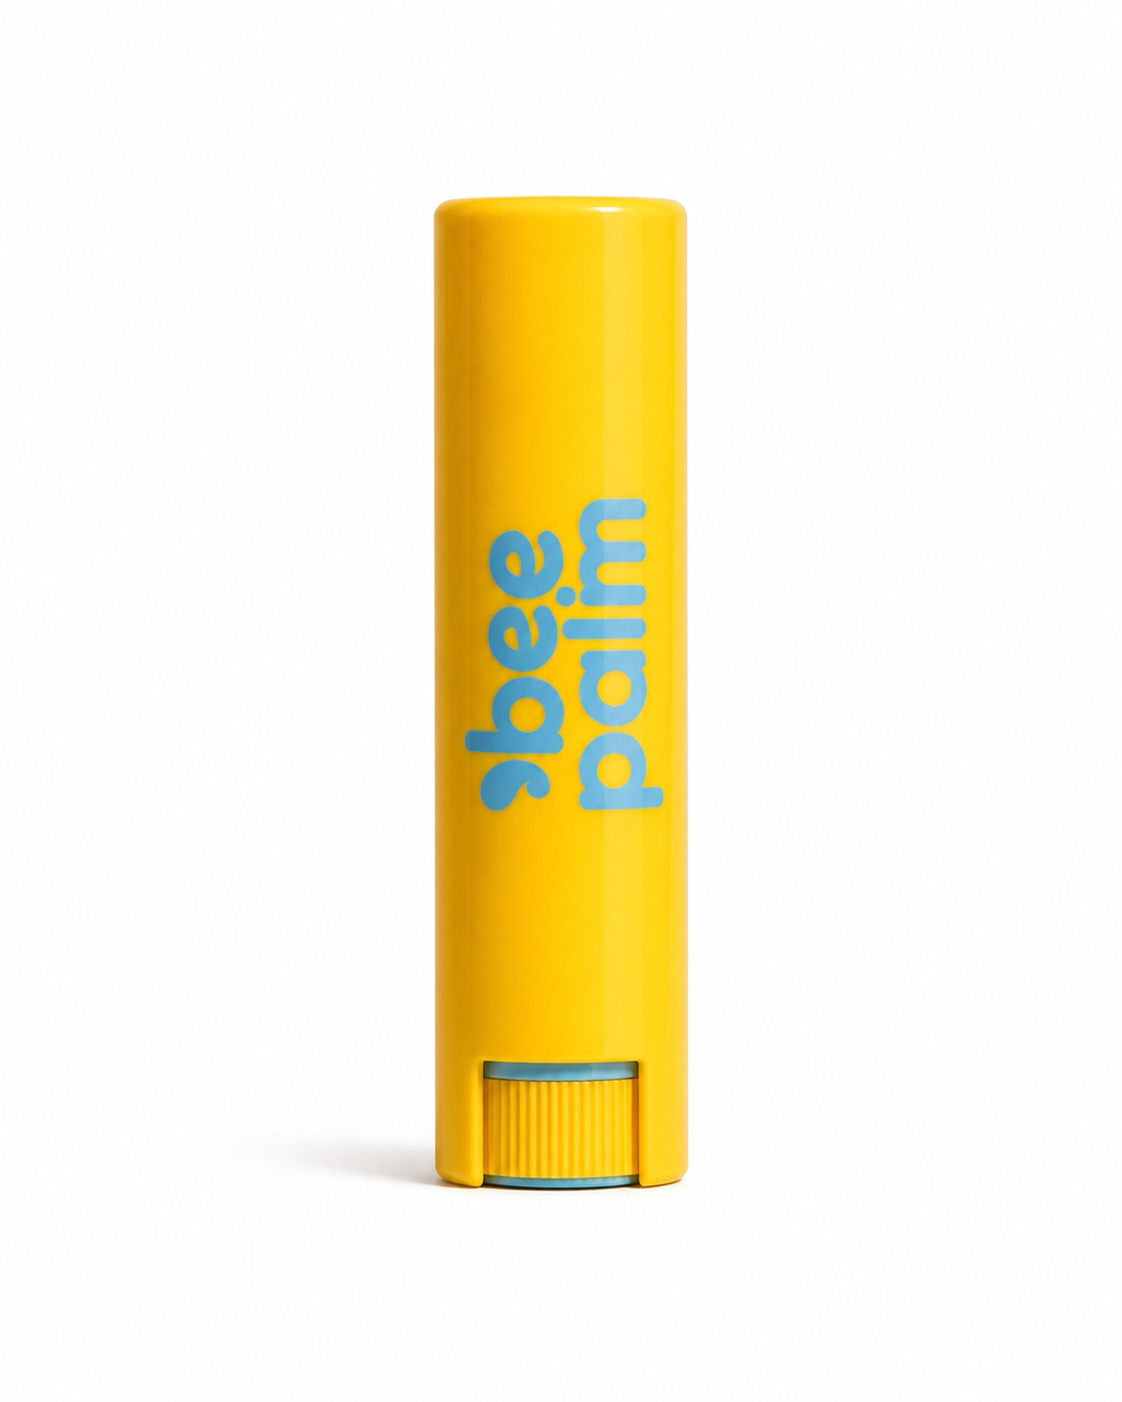
\includegraphics[width=0.5\textwidth]{sample-prod-1}
  \caption{\emph{bee palm} lip balm tube concept render. The brand mark is placed on the tube in the brand's primary yellow; the framing is honest concept material rather than a manufactured-product photograph.}
  \label{fig:appproduct1}
\end{figure}

\begin{figure}[ht!]
  \centering
  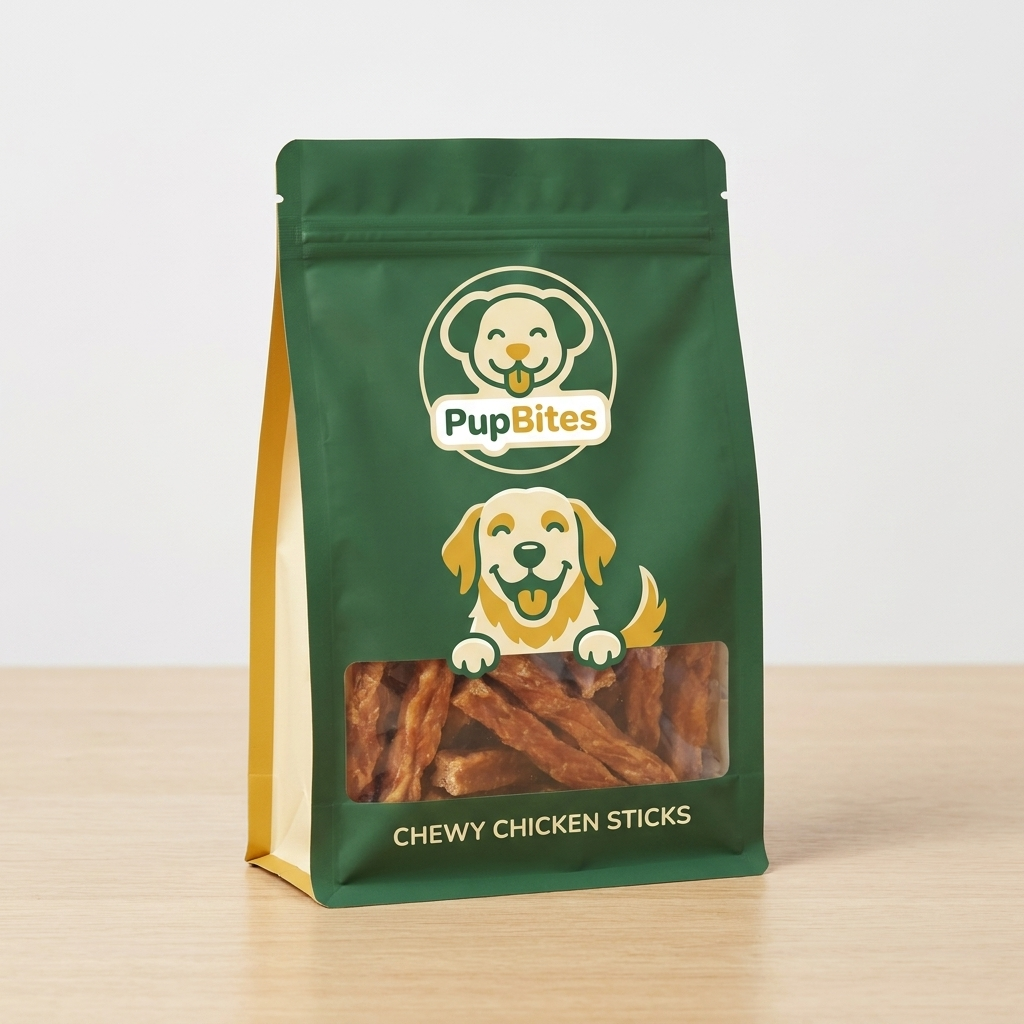
\includegraphics[width=0.7\textwidth]{sample-prod-2}
  \caption{\emph{PupBites} \textit{Chewy Chicken Sticks} packaging concept. The logo from \cref{fig:applogos3} is placed on the front of a stand-up pouch with a product window; the framing reads as a feed-style product photograph rather than as a packshot on a white background.}
  \label{fig:appproduct2}
\end{figure}

\section{Sample generated ad}

\Cref{fig:appad1} shows one generated 4:5 static feed ad from the bee palm campaign. The ad carries the on-image headline, primary line, CTA, and the price + sale-percentage badges driven by the optional promo fields on the brand panel.

\begin{figure}[ht!]
  \centering
  
\includegraphics[width=0.6\textwidth]{sample-ad-1}
  \caption{\emph{bee palm} Stage~3 sales creative. The on-image typography pulls from the brand's primary blue; the price (\$4.99) and the 20\% off badge are rendered onto the image because the user filled both promo fields on the brand panel. The CTA reflects the WhatsApp business model selected on the brief (``Text Us To Stock Up'') rather than a generic Shop Now.}
  \label{fig:appad1}
\end{figure}


\end{document}
